\documentclass[a4paper, 11pt]{article}
\usepackage[utf8]{inputenc}

%margin
\usepackage[margin=2cm]{geometry}
%\usepackage{geometry}
%lists
\usepackage{enumitem}
%encoding
\usepackage[utf8]{inputenc}
\usepackage[T1]{fontenc}
%English
\usepackage[english]{babel}
%colors
\usepackage[dvipsnames,svgnames,table]{xcolor}
%tables
\usepackage{multirow}
%for math
\usepackage{amsfonts}
\usepackage{amssymb}
\usepackage{mathrsfs}
\usepackage{amsmath}
\usepackage{amsthm}
\usepackage{mathtools}
\usepackage{nicefrac}
%for images
\usepackage{graphicx}
%for plots
\usepackage{tikz}
\usetikzlibrary{mindmap}
%links
\usepackage{hyperref}
%citations
\usepackage{natbib}
\setcitestyle{numbers, notesep={: }}


%environments
\newtheorem*{notation}{Notation}
\newtheorem{definition}{Definition}[section]
\newtheorem{proposition}{Proposition}[section]
\newtheorem{property}{Property}[section]
\newtheorem{lemma}{Lemma}[section]
\newtheorem{theorem}{Theorem}
\newtheorem{corollary}{Corollary}[section]
%commands
%\newcommand{\name}[num]{definition}
\newcommand{\primes}{\mathbb{P}}
\newcommand{\N}{\mathbb{N}}
\newcommand{\Z}{\mathbb{Z}}
\newcommand{\Q}{\mathbb{Q}}
\newcommand{\D}{\mathbb{D}}
\newcommand{\R}{\mathbb{R}}
\newcommand{\C}{\mathbb{C}}
\newcommand{\F}{\mathbb{F}}
\newcommand{\halfplane}{\mathbb{H}}
%\newcommand{\dim}[1]{\text{dim}(#1)}
\newcommand{\floor}[1]{\lfloor #1 \rfloor}
\newcommand{\ceil}[1]{\lceil #1 \rceil}
\newcommand{\curt}[1]{\sqrt[3]{#1}}
\newcommand{\Ker}[1]{\text{Ker}(#1)}
\newcommand{\Image}[1]{\text{Im}(#1)}
\newcommand{\Gal}[1]{\text{Gal}(#1)}
\newcommand{\Frob}[2]{\text{Frob}_{#1}(#2)}

    
%opening
\title{Modular forms modulo 2}
\author{Paul Dubois}
%\date{2019/2020}


%\includeonly{ModularForms,ModularFormsModuloTwo}
%\includeonly{FrobenianMaps}




\begin{document}
\maketitle

\begin{abstract}
We are interested in Modular forms modulo 2, and computing thing about it.
[temporary abstract]

Key words that should appear:
Modular forms;
Mod 2;
Duality of definitions;
Governing fields;
Frobenian map?;
Exact computations;
\end{abstract}

\tableofcontents



\section{Modular forms}
\subsection{Modular forms of level 1}
Let $\halfplane$ denote the upper-half plane, that is, $\halfplane = \{z = x+yi \in \C | \ y>0 \}$.

We say that a function $f:\halfplane \to \C$ is \textit{weakly modular} of \textit{weight} $2k$ if $f$ is meromorphic and
$$
f(z) = (cz+d)^{-2k} f \left( \frac{az+b}{cz+d} \right)
\qquad \text{ for all }
\begin{pmatrix} a & b\\
				c & d
\end{pmatrix}
\in \SL2{\Z}.
$$

The group $\SL2{\Z}$ of invertible $(2x2)$ matrices over $\Z$ with  is generated by
$$
S = \begin{pmatrix} 0 & -1 \\
					1 &  0
\end{pmatrix}
\quad \text{ and } \quad
T = \begin{pmatrix} 1 & 1 \\
					0 & 1 
\end{pmatrix};
$$
see \cite[p.1-2]{SL2Z}.

From this property, we can derive an alternative definition of weakly modular functions:
$f$ is weakly modular of weight $2k$ if $f$ is meromorphic and
$$
f(z+1) = f(z) \quad \text{ and } \quad f(-1/z) = z^k f(z)
$$
for all $z \in \C$.

Moreover, we define a function $f:\halfplane \to \C$ to be \textit{modular} of weight $2k$ if $f$ is holomorphic and weakly modular.
Lastly, we say that a function $f:\halfplane \to \C$ is a \textit{modular form} of weight $2k$ if it modular and holomorphic at $\infty$, that is, $f(\nicefrac{1}{z})$ is holomorphic at $z=0$.

It is straightforward to check, using the above definition, that the set of modular forms of weight $2k$ is closed under addition and multiplication by complex scalars.
More precisely:
\begin{itemize}
    \item If $f_1$ and $f_2$ are modular forms of weight $2k$, then $f_1+f_2: z \to f_1(z)+f_2(z)$ is modular of weight $2k$ as well.
    
    \item Similarly, if $\lambda \in \C$ and $f$ is a modular form of weight $2k$, then so is $\lambda \cdot f: z \to \lambda f(z)$.
\end{itemize}
Therefore, modular forms of weight $2k$ over $\C$ form a space. We denote it $M_k$.

It is also possible to multiply modular forms, in which case the weights are additive:
If $f_1$ and $f_2$ are modular forms of respective weights $2k_1$ and $2k_2$, then $f_1f_2:a \to f_1(z)f_2(z)$ is modular of weight $2k_1+2k_2$.

We deduce that we can take powers of modular forms, and the weight is then multiplied by the exponent:
if $f(z)$ is modular of weight $2k$, then $f^n(z)$ is modular of weight $2k \cdot n$ (with $n \in \N$).



\subsection{Typical Modular Forms}
\subsubsection{Eisenstein series $G_k$}
The most famous class of modular forms is probably the Eisenstein series, usually denoted $G_k$. We define them as follows \cite[Examples of Modular Forms of Level 1]{ModularFormsComputationalApproach}:
$$
G_k(z) = \sum_{(m,n) \in \Z^2\setminus\{(0,0)\}} \frac{1}{(mz+n)^{2k}}
$$
for $k \geq 2$.

It is easy to check that $G_k$ are modular of weight $2k$ \cite[Proposition 2.1]{ModularFormsComputationalApproach}, as:
$$
G_k(z+1) = G_k(z)
$$
(using $(m,n+m) \to (m,n)$, an invertible map)
$$
G_k(-1/z) = z^k G_k(z)
$$
(using $(m,-n) \to (m,n)$, an invertible map).

It is pleasant to remark that \cite[Proposition 2.2]{ModularFormsComputationalApproach}
$$
G_k(\infty) = \sum_{n \in \Z^*} \frac{1}{n^{2k}} = 2\zeta(2k)
$$.
Where $\zeta(k)$ is Riemann zeta function.
The values of this function are well-known on positive even numbers, and we deduce \cite[p.194]{MathHandbook} that:
$$
G_k(\infty) = 2\zeta(2k) = \frac{(2\pi)^{2k}}{(2k)!}B_k
$$
where $B_k = (-1)^{k+1} b_{2k}$ and $b_k$ are Bernoulli numbers.

\subsubsection{The Modular Discriminant $\Delta$}
We will be interested in one main modular form in the rest of this article: the modular discriminant $\Delta$.
We define $\Delta$ in terms of $G_k$ as follows \cite[p.84]{CourseInArithmetic}:
$$
\Delta = \left( \frac{1}{(2\pi)^{12}} \right) (g_2^3 - 27g_3^2) \in M_6^0 \qquad \text{ with } g_2 = 40G_2 \text{ and } g_3 = 140G_3
$$
As $g_2^3$ is modular of weight $4 \cdot 3=12$ and $g_3^2$ of weight $6 \cdot 2 = 12$, $\Delta$ is modular of weight $12$.
Multiplying by the scalar $\left( \nicefrac{1}{(2\pi)^{12}} \right)$ doesn't change the weight of the modular form, and it will we useful later for normalization purposes.

Now, using 
$
G_2(\infty) = 2\zeta(4) = \frac{\pi^4}{45}
$
 and 
$
G_3(\infty) = 2\zeta(6) = \frac{2\pi^4}{945}
$
, we get 
$$
\Delta(\infty) = \left( \frac{1}{(2\pi)^{12}} \right) \left[ \left( \frac{4\pi^4}{3} \right)^3 - \left( \frac{8\pi^4}{27} \right)^2 \right] =  0
$$
so $\Delta$ has a zero at infinity.


\subsection{Cusp Forms}
A function $f:\halfplane \to \C$ that is a modular form may in addition be a cusp form, if $f(\infty)=0$.
We will denote the space of modular cusp forms of weight $2k$ over $\C$ by $M_k^0$.

It is useful to note $G_k(\infty) = \sum_{n \in \N^*} \frac{2}{n^{2k}} > 2$ and in particular, $G_k(\infty) \neq 0$, so $G_k$ are \textit{not} cusp forms for any $k$.
As we have shown it before, $\Delta(\infty)=0$, so $\Delta$ is a modular cusp form of weight 12, so $\Delta \in M_6^0$.
Using tools from complex analysis, we can prove that $\Delta$ has only one zero (at infinity), which has order one \cite[p.88]{CourseInArithmetic}.
%[proof?]

We have the following relation: 
\begin{theorem}
    $M_k \cong M_k^0 \oplus \C \cdot G_k \quad \text{ for all } k \geq 2$ \cite[p.88]{CourseInArithmetic}
\end{theorem}
\begin{proof}
    We let $\Phi:M_k \to \C$ such that if $f \in M_k$, $\Phi(f) = f(\infty)$.
    
    Now, we have $\Ker{\Phi} = M_k^0$, therefore, by the 1\textsuperscript{st} Isomorphism Theorem, $\nicefrac{M_k}{M_k^0} \cong \Image{\Phi} \subseteq \C$.
    
    Note that $G_k \in M_k$, and $G_k(\infty) = \sum_{n \in \Z^*} \frac{1}{n^{2k}} \neq 0$, so $G_k \not\in M_k^0$.
    As $G_k \neq 0$, $\dim(\nicefrac{M_k}{M_k^0}) \geq 1$ and $\Image{\Phi} = \C$.
    Thus, $G_k \in M_k\\M_k^0$
    
    Finally, we have $M_k \cong M_k^0 \oplus \C.G_k$ if $k \geq 2$.
    (The above argument fails for $k<2$ as $G_k$ is not well defined any more.)
\end{proof}
Therefore, the dimensions of $M_k$ and $M_k^0$ are closely linked.



\subsection{Dimensions of Spaces of Modular Forms}
The fact that multiplying two modular forms gives a function that remains modular yields that we may map a set of modular forms to an other.

\begin{theorem}
    $M_{k-6} \cong M_k^0$. \cite[p.88]{CourseInArithmetic}
\end{theorem}
\begin{proof}
    We let $\Phi:M_{k-6} \to M_k^0$ such that if $f \in M_k$, $\Phi(f)(z) = \Delta(z)f(z)$.
    
    This is well defined as if $f$ has weight $2(k-6)$, $\Delta.f$ has weight $2k$ since $\Delta$ has weight $12$. As $\Delta$ is a cusp from, $\Delta.f$ will also be a cusp form.
    
    From definition, $\Phi$ is clearly homomorphic.
    
    
    Now, if $g \in M_k^0$, we may define $\Psi: M_k^0 \to M_{k-6}$ such that $\Psi(g)(z) = \nicefrac{g(z)}{\Delta(z)}$
    
    This is well defined as if $g$ has weight $2k$, $\Delta.f$ has weight $2k$ since $\Delta$ has weight $12$. As $\Delta$ is a cusp from, $\Delta.f$ will also be a cusp form.
    
    This is well defined as $\Delta$ has only one zero, at infinity, where $g$ also has a zero (as $g$ is a cusp form). The weights agree again as well.
    
    It is then easy to remark that $\Psi = \Phi^{-1}$. So $\Phi$ is bijective, and thus isomorphic. 
    
    Finally, we have $M_{k-6} \cong M_k^0$.
\end{proof}
This theorem, combined with the previous one is very powerful: it shows that there must be a pattern (of 6) in the sequence of dimensions $\dim(M_k)$ and $\dim(M_k^0)$ for $k \geq 2$.
We have $M_k \cong M_k^0 \oplus \C.G_k \cong M_{k-6} \oplus \C.G_k$, so $\dim(M_k) = \dim(M_{k-6})+1$ when $k \geq 2$.
Thus, if we compute the dimensions of $M_0$, $M_1$, $M_2$, $M_3$, $M_4$, $M_5$, we can extrapolate dimensions of $M_k$ and $M_k^0$ for all $k$.

Using complex analysis techniques again, we have:
\begin{itemize}
    \item $\dim(M_k) = 0 \quad k < 0$
    \item $\dim(M_1) = 0$
    \item $\dim(M_0) = \dim(M_2) = \dim(M_3) = \dim(M_4) = \dim(M_5) = 1$
\end{itemize}
%[proof?]
In the case $k=0$, $\dim(M_0) = 1$. As $f(z) = 1$ is clearly a modular from of weight $0$, $\{1\}$ is a basis for $M_0$. We deduce $\dim(M_k^0) = 0$ as $1$ is clearly not a cusp form.
In the case $k=1$, $\dim(M_1) = 0$, which makes $\dim(M_1^0) = 0$ automatically.
(Cases $k<0$ are similar to $k=1$.)

Other cases may be derived directly from the relations (using induction to get general formulas), and we obtain:

%[Table of dimensions of $M_k$ and $M_k^0$]
\begin{center}
\begin{tabular}{||c||c|c|c||} 
    \hline
    Space & $k<0$ & $k \geq 0, \ k \equiv 1 \bmod 6$ & $k \geq 0, \ k \not \equiv 1 \bmod 6$ \\
    \hline
    \hline
    $\dim(M_k)$ & $0$ & $\floor{\nicefrac{k}{6}}$ & $\floor{\nicefrac{k}{6}} + 1$ \\
    \hline
    $\dim(M_k^0)$ & $0$ & $\max\{0, \floor{\nicefrac{k}{6}} - 1\}$ & $\floor{\nicefrac{k}{6}}$ \\
    \hline
\end{tabular}
\end{center}
Note that the $\max$ is taken only to avoid negative dimensions.



\subsection{Fourier Expansion}
\subsubsection{Definition}
To study such function, we use Fourier Expansion.
In the case of $f$ being a modular form of weight $2k$, 
a Fourier Expansion is a representation of $f$ as a power series of $e^{2\pi i n z}$
i.e. $$f(z) = \sum_{n \in \Z} a_n(f) e^{2\pi inz}.$$
We usually denote $q = e^{2\pi i z}$ so that $q^n = e^{2\pi i n z}$ 
and the Fourier expansion of $f$ become 
$$
f(q) = \sum_{n \in \Z} a_n(f) q^n.
$$
When in this form, we may as well call it the $q$-expansion.

\subsubsection{Typical Modular Forms Fourier Expansion}
\paragraph{Fourier Expansions of $G_k$}
The modular forms $G_k$ have the following $q$-expansion \cite[p.92]{CourseInArithmetic}:
$$
G_k(q) = 2\zeta(2k) + 2 \frac{{(2 \pi i)}^{2k}}{(2k-1)!} \sum_{n=1}^{\infty} \sigma_{2k-1}(n)q^n
$$
where $\sigma_d$ is the generalized divisor function such that:
$$
\sigma_d(n) = \sum_{m \mid n} m^d
.$$
%[proof?]

\paragraph{Fourier Expansion of $\Delta$}
We also have \cite[p.95]{CourseInArithmetic}:
$$
\Delta(q) = q \prod_{n=1}^{\infty} (1-q^n)^{24}
$$
%[Proof?]



\subsection{A Basis for Modular Forms}
\label{BasisModularForms}
The set of modular forms that are weight $2k$ in fact form a vector space (we can add modular forms together, and multiply them with a constant) over the complex numbers. 
One may ask then a basis for this vector space.

We would like to find a basis for each set $M_k$. It turns out that the modular forms $G_2$ and $G_3$ introduced before in fact generate a basis for all $M_k$. 
It is not obvious and may in fact seems wrong at a first stage: $G_2$ and $G_3$ are modular forms of weight $4$ and $6$, whereas $M_k$ in general have modular forms of weight $2k$.
However, by taking combinations of $G_2$ and $G_3$, we may obtain modular forms of any weight $2k$. It is important to remember that when multiplied, the weight of modular forms add up.

\begin{theorem}
    The set $S = \{G_2^aG_3^b | a,b \in \N, 2a+3b = k\}$\footnote{The set of naturals $\N$ is taken to start from $0$.} is a basis for $M_k$. \cite[Theorem 2.17]{ModularFormsComputationalApproach}
\end{theorem}
\begin{proof}
    Of course, the cases when $\dim(M_k)=0$ (for $k<0$ and $k=1$) are trivial, as the basis is empty, and $2a+3b = k$ has no solution for $a,b \in \N$.
    
    To show $S$ is a basis, we need it to span $M_k$ and to be linearly independent.
    
    We start with spanning, and we proceed by induction on $k$, with step $6$.
    
    As $\dim(M_k)=1$ for $k=0,2,3,4,5,7$, and the equation $2a+3b = k$ has exactly one solution for $a,b \in \N$ (namely $(a,b)=(0,0), (1,0), (0,1), (2,0), (1,1), (2,1)$), $S$ has only one element, which must be the basis.
    
    Now, for $k>7$, take some $a,b \in \N$ such that $2a+3b=k$. Let $f \in M_k$, and $g = G_2^aG_3^b \in M_k$.
    $g(\infty) \neq 0$ as none of $G_2$ or $G_3$ is a cusp form. 
    So there must be a complex $\lambda$ such that $f - \lambda g$ is a cusp form. 
    Then $f - \lambda g \in M_k \cong M_{k-6}^0$ and we can find a $h \in M_{k-6}^*$ such that $h.\Delta = f - \lambda g$.
    
    By induction, $h$ must be a polynomial of $G_2$ and $G_3$; by definition, $\Delta$ is one as well (note that yet, we don't put any restriction on powers of $G_2$ and $G_3$, other then being positive integers).
    Therefore, $f = \Delta.h + \lambda g$ is a polynomial of $G_2$ and $G_3$.
    From the fact that $f \in M_k$ (i.e. $f$ has weight $2k$), terms of $f$ as a polynomial of $G_2$ and $G_3$ have the from $G_2^aG_3^b$ with $2a+3b=k$.
    
    We now want to show linear independence, we proceed by contradiction.
    
    Suppose there is a non-trivial linear relation of terms $G_2^aG_3^b$. 
    We can multiply it by suitable $G_2$ and $G_3$ so that all terms have the form $2a+3b = k \equiv 0 \bmod 12$.
    Then, we can divide all terms by $G_3^2$, witch gives us that there is a polynomial for which $\nicefrac{G_2^3}{G_3^2}$ is a root.
    In particular, this polynomial is constant when $\nicefrac{G_2^3}{G_3^2}$ is plugged.
    This contradicts the fact that $q$-expansion of $\nicefrac{G_2^3}{G_3^2}$ is not constant.
\end{proof}

This set of makes to be a basis, and one may even find it pleasant: given the two modular forms $G_2$ and $G_3$, this set generates all the modular forms of weight $2k$ that we could think of, if we only knew these two modular forms.



\subsection{Hecke Operators}
\label{DefHeckeOperators}
We define the Hecke operators for a modular form $f$ as follows \cite[p.100]{CourseInArithmetic}:
$$
T_nf(z) = n^{2k-1}\sum_{a \geq 1,\, ad=n,\, 0 \leq b < d} d^{-2k}f \left( \frac{az+b}{d} \right)
$$
with $n \in \N$.

We can check that $T_nf$ is modular if $f$ is (as the sum of modular forms).

%[properties of T_n? (T_{mn} and T_pT_{p^n})]

We may as well write $T_nf$ as a Fourier Expansion of $q=e^{2 \pi i z}$ as follows \cite[p.100]{CourseInArithmetic}:
$$
T_nf(z) = \sum_{m \in \Z} \gamma(m)q^m
\quad \text{ with } \quad 
\gamma(z) = \sum_{a | (n,m),\, a \geq 1} a^{2k-1} c\left( \frac{mn}{a^2} \right)
$$
$$
\text{For modular forms } f \text{ s.t. }
f(z) = \sum_{n \in \Z} \alpha(n)q^n
$$
%[proof?]





% !TeX spellcheck = en_GB
\section{Modular Forms Modulo Two}
\subsection{Strategy to Reduce Modulo Two}
It is not trivial, at this point, why and how we can reduce modulo 2 modular forms, objects that have coefficients in $\C$.
In general, reduction modulo a number is only possible with whole numbers (integers).
We would like to reduce modulo 2 coefficients of the Fourier series for modular forms.
But at the moment, they lie in $\C$.

In fact, we will introduce a new basis for the modular forms: the so called Miller Basis.
The coefficients of all the forms in this basis are integers. It is then possible to consider the space of modular forms over $\Z$ instead of $\C$.
Once this is done, we will reduce all the newly integral coefficients modulo $2$.

In this section, we will denote all objects reduced modulo 2 with an $\overline{\text{over-line}}$:
\begin{itemize}
	\item The modular form $f$ once reduced will be denoted $\overline{f}$.	\item The coefficients of the $q$-expansion $c$ will reduce to $\overline{c}$
	\item The Hecke operators $T_n$ reduced will be denoted $\overline{T_n}$.
\end{itemize}

\subsection{Integral Basis}
\subsubsection{Normalisation of Typical Modular Forms}
\paragraph{Normalisation of Eisenstein series $G_k$}
We first recall the formula for $q$ extension of $G_k$ and the one for $\zeta(2k)$:
$$
G_k(q) = 2\zeta(2k) + 2 \frac{{(2 \pi i)}^{2k}}{(2k-1)!} \sum_{n=1}^{\infty} \sigma_{2k-1}(n)q^n
$$
and
$$
2\zeta(2k) = \frac{(2\pi)^{2k}}{(2k)!}B_k
$$
so overall:
$$
G_k(q) = \frac{(2\pi)^{2k}}{(2k)!}B_k + 2 \frac{{(2 \pi i)}^{2k}}{(2k-1)!} \sum_{n=1}^{\infty} \sigma_{2k-1}(n)q^n
$$

We would like to normalize this series, so that the coefficients become integers, so that we can ultimately reduce them modulo 2.
Right now, coefficients are rational.

As we want to keep the series modular with same weight, the only tool we have to normalize the series is multiplication by a constant.
The normalization is a crucial point: 
If we multiply by $2$ all coefficients of a modular form that already lie in $\Z$, the reduction $\bmod 2$ will always give zero.

First, let's normalize the series to have particular values on some coefficients of interest.
There are two justified ways to do so: normalize to have constant coefficient set to one, and to have $q$ coefficient is set to one.
We will introduce both:
Let $E_k$ be such that:
$$
E_k.2\zeta(2k) = G_k
$$
so that
$$
E_k = 1 + (-1)^k \frac{4k}{B_k} \sum_{n=1}^{\infty} \sigma_{2k-1}(n)q^n.
$$
$E_k$ then has constant coefficient set to one.

Let $F_k$ be such that:
$$
F_k.\left( 2 \frac{{(2 \pi i)}^{2k}}{(2k-1)!} \right) = G_k
$$
so that
$$
F_k =  (-1)^k \frac{B_k}{4k} + \sum_{n=1}^{\infty} \sigma_{2k-1}(n)q^n.
$$
$F_k$ then has $q$-coefficient set to one (as $\sigma_{2k-1}(1)=1$).

Clearly, the coefficients of this expansion remain in $\Q$ at least, and we will show that for some specific $k$, the coefficients lie in fact in $\Z$.
Both $F_k$ and $E_k$ are interesting, but for our purpose (reducing modulo 2), we will use $E_k$.
Note that $E_k$ are normalized versions of Eisenstein series $G_k$, but in literature, both are called Eisenstein series see \cite[p.6]{IntoductionModularFormsWorkshop} for example.

\paragraph{The Modular Discriminant $\Delta$ Normalized}
Again, we recall the formula for $q$ extension of $\Delta$:
$$
\Delta(q) = q \prod_{n=1}^{\infty} (1-q^n)^{24}
$$
Clearly, the coefficients in expansion of $\Delta$ are integers (which we can reduce modulo 2).
This is the reason why we defined $\Delta$ with the $\frac{1}{(2\pi)^{12}}$ factor in front.


\subsubsection{Miller Basis}
\paragraph{Basis with Integral Coefficients (in Fourier Series)}
Applying normalization $G_k \to E_k$ above for $k=2,3$, we get:
\begin{align*}
	E_2 &= 1 + \frac{8}{B_2} \sum_{n=1}^{\infty} \sigma_{3}(n)q^n \qquad B_2 = \frac{1}{30} \\
	    &= 1 + 240 \sum_{n=1}^{\infty} \sigma_{3}(n)q^n
\end{align*}

and
\begin{align*}
	E_3 &= 1 - \frac{12}{B_3} \sum_{n=1}^{\infty} \sigma_{5}(n)q^n \qquad B_3 = \frac{1}{42} \\
	    &= 1 - 504 \sum_{n=1}^{\infty} \sigma_{5}(n)q^n
\end{align*}

Now, we have shown that $\{G_2^aG_3^b | 2a+3b=k\}$ is a basis for modular forms of weight $2k$ over the complex (see \ref{BasisModularForms}).
As $E_2 = \lambda G_2,\ \lambda \in \C$ and $E_3 = \mu G_3,\ \mu \in \C$, we have that $\{E_2^aE_3^b | 2a+3b=k\}$ remains a basis for $M_k$ over $\C$.

It is clear, from the series, that coefficients of the $q$-expansion of both $E_2$ and $E_3$ are all integers.
Thus, so are coefficients of combinations of $E_2$ and $E_3$.
Therefore, we have found a basis for $M_k$ such that all elements in the basis have only integral coefficients in their $q$-expansion.
\label{IntegralBasisModularForms}

\paragraph{Miller Basis for $M_k^0$}
This is a nice result, but we can in fact do better, by forcing the first coefficients to chosen values.

\begin{theorem}
	For the space of modular cusp forms $M_k^0$, there exists a basis $\{f_1, \cdots, f_r\}$ such that:
	\begin{itemize}
		\item $f_i \in Z[q]$
		\item $ a_i^j = \delta_ij = 
		\left\lbrace
		\begin{array}{l l}
			1 & \text{ if } i   =  j \\
			0 & \text{ if } i \neq j
		\end{array}
		\right. \quad
		\forall 1 \leq i,j \leq r$\\
		where $a_i^j$ is the coefficient of $q^j$ in expansion of $f_i$.
	\end{itemize}
\end{theorem}
This is commonly called the Miller basis for $M_k^0$, as it was first introduced by Victor Saul Miller \cite{MillerThesis}.
\begin{proof}
	\begin{itemize}
		%boring part
		\item For $k<6$, $k=7$, we have $\dim(M_k^0)=0$.
		Thus, $\emptyset$ is a basis which satisfies the Miller basis properties.
		
		%semi-boring part
		\item For $k=6$, we have $\dim(M_k^0)=1$.
		Thus, $\{ \Delta \}$ is a basis which satisfies the Miller basis properties.
		
		%interesting part
		\item For $k \geq 7$, we let $r = \dim(M_k^0) \geq 1$.	
		We then consider the set
		$$
		\{ g_j | 1 \leq j \leq r \}
		$$
		where
		$$
		g_j = \Delta^jE_3^{2(d-j)+b}E_2^a
		$$
		with
		$$
		2a+3b \leq 7 \ \&\ 2a+3b \cong k \bmod 6$$
		$$
		\& \ \ d=\frac{k-(2a+3b)}{6} \quad \in \N \text{ as $k \geq 7$}
		$$
		Note that $a$ and $b$ are unique unless $k \cong 0 \bmod 6$. In witch case, we use by convention $a=0$, $b=0$.
		
		As all $E_2$, $E_3$, and $\Delta$ have integral coefficients, $g_j$ will as well.
		
		We then look at the $q$ series:
		$$
		\Delta(q) = q + O(k^2) \implies \Delta^j(q) = q^j + O(k^{j+1})
		$$
		As we normalized so,
		$$
		E_2(q) = 1 + O(q) \implies E_2^{\alpha}(q) = 1 + O(q)
		$$
		$$
		E_3(q) = 1 + O(q) \implies E_3^{\alpha}(q) = 1 + O(q)
		$$
		
		This gives:
		$$
		g_j(q) = q^j + O(q^{j+1}) \quad \forall 1 \leq j \leq r.
		$$
		Therefore, $\{ g_j, | 1 \leq j \leq r \}$ is clearly a linearly independent set. By dimension argument, it also spans $M_k^0$. Therefore, it forms a basis.
		Moreover, in this basis: $a_i^j = \delta_{ij} \quad i \leq j$.
		
		Finally, we can use Gaussian elimination on $\{g_j\}$ to obtain a basis $\{f_j | 1 \leq j \leq r \}$ such that: $a_i^j = \delta_{ij} \quad \forall 1 \leq i,j \leq r$.
		The coefficients will remain in $\Z$ after Gaussian elimination.
	\end{itemize}
\end{proof}

\paragraph{Extension to all $M_k$}
We already have a basis for $M_k^0$, as $\dim(M_k) = \dim(M_k^0) + 1$ (over $\C$), we just need to adjoint one element of $M_k \setminus M_k^0$ to our basis.

It was shown before that $\{E_2^aE_3^b | 2a+3b=k\}$ is a basis for $M_k$ with integral coefficients (see \ref{IntegralBasisModularForms})
One may see from the $q$-expansion that $E_2^aE_3^b = 1 + O(q)$ so $E_2^aE_3^b \in M_k \setminus M_k^0$.

Therefore, we can just add one element of $\{E_2^aE_3^b | 2a+3b=k\}$ to the Miller basis, and use Gaussian elimination again.
We get a basis foe $M_k$ of the form $\{f_j | 0 \leq j \leq r \}$ such that in this basis: $a_i^j = \delta_{ij} \quad \forall 0 \leq i,j \leq r$ (with $r=dim(M_k^0)$ i.e. $r+1=dim(M_k)$).

\paragraph{Miller Basis Examples}
\subparagraph{Miller basis for $k=16$}
We can calculate the Miller basis for $k=16$:
$k \cong 4 \bmod 12$ so $a=2$ and $b=0$; $d=2$.
We put $g_1 = \Delta^1E_3^2E_2^2$, so:
\begin{align*}
    g_1(q) &= \Delta(q)E_2^2(q)E_3^2(q)\\
           &= \left[ q - 24q^2 + 252q^3 + O(q^4) \right]\\
           & \qquad \cdot \left[ 1 + 240q + 2160q^2 + 6720q^3 + O(q^4) \right]^2\\
           & \qquad \qquad \cdot \left[ 1 - 504q - 16632q^2 + 122976q^3 + O(q^4) \right]^2\\
           &= q - 552q^2 - 188244q^3 + O(q^4)
% (Wolfram|Alpha) develop (q - 24q^2 + 252q^3)(1 + 240q + 2160q^2 + 6720q^3)^2(1 - 504q - 16632q^2 + 122976q^3)^2
\end{align*}
and $g_2 = \Delta^2E_3^0E_2^2$, so:
\begin{align*}
    g_2(q) &= \Delta^2(q)E_2^2(q)\\
           &= \left[ q - 24q^2 + 252q^3 + O(q^4) \right]^2\\
           & \qquad \cdot \left[ 1 + 240q + 2160q^2 + 6720q^3 + O(q^4) \right]^2\\
           &= q^2 + 432q^3 + O(q^4)
% (Wolfram|Alpha) develop (q - 24q^2 + 252q^3)^2(1 + 240q + 2160q^2 + 6720q^3)^2
\end{align*}
Then, $f_2=g_2$ and $f_1=g_1+552g_2$, so:
\begin{align*}
    f_1(q) &= q - 552q^2 - 188244q^3 + O(q^4) \ + \ 552 \cdot \left[q^2 + 432q^3 + O(q^4)\right] \\
           &= q + 50220q^3 + O(q^4)\\
    f_2(q) &= q^2 + 432q^3 + O(q^4)\\
% (Wolfram|Alpha) develop q - 552q^2 - 188244q^3 + 552 \cdot [q^2 + 432q^3]
\end{align*}

Therefore, up to $O(q^4)$, $\{f_1, f_2\}=\{q + 50220q^3 + O(q^4), q^2 + 432q^3 + O(q^4)\}$ is a basis for $M_{16}^0$.

To extend this base to $M_k$, we adjoint a term of the form $g_0 = E_2^aE_3^b$ where $2a+3b=16$. We pick $g_0 = E_2^8$, so:
\begin{align*}
    g_0(q) &= E_2^8(q)\\
           &= \left[ 1 + 240q + 2160q^2 + 6720q^3 + O(q^4) \right]^8\\
           &= 1 + 1920q + 1630080q^2 + 803228160q^3 + O(q^4)
% (Wolfram|Alpha) develop (1 + 240q + 2160q^2 + 6720q^3)^8
\end{align*}
Then, $f_0 = g_0 - 1920g_1 - 1630080g_2$, so:
\begin{align*}
    f_0(q) &= g_0(q) - 1920g_1(q) - 1630080g_2(q)\\
           &= \left[ 1 + 1920q + 1630080q^2 + 803228160q^3 + O(q^4) \right]\\
           & \qquad - 1920 \left[ q + 50220q^3 + O(q^4) \right] \\
           & \qquad \qquad - 1630080 \left[ q^2 + 432q^3 + O(q^4) \right]\\
           &= 1 + 2611200q^3 + O(q^4)
% (Wolfram|Alpha) develop [1 + 1920q + 1630080q^2 + 803228160q^3] - 1920\cdot[q + 50220q^3] - 1630080\cdot[q^2 + 432q^3]
\end{align*}

Therefore, up to $O(q^4)$, $\{f_0, f_1, f_2\} = \{1 + 2611200q^3 + O(q^4), q + 50220q^3 + O(q^4), q^2 + 432q^3 + O(q^4)\}$ is a basis for $M_{16}$.

\subparagraph{Miller basis for $k=92$}
The calculation of this basis may be interesting by hand once;
However, it is possible to automate it.
The procedure that calculates such coefficients is a standard in SageMath \cite{sage}.
Here is, up to $O(q^{10})$, the Miller basis for $M_{92}$:
% (sage) victor_miller_basis(92, prec=10, cusp_only=False, var='q')
\begin{align*}
	f_0 &= 1 + 3034192667130000 q^8 + 137290127714549760000 q^9 + O(q^{10})\\
	f_1 &= q + 91578443563200 q^8 + 2651503140376278561 q^9 + O(q^{10})\\
	f_2 &= q^2 + 2380310529376 q^8 + 42238207588515840 q^9 + O(q^{10})\\
	f_3 &= q^3 + 51682260816 q^8 + 530253459731160 q^9 + O(q^{10})\\
	f_4 &= q^4 + 896013480 q^8 + 4882999541760 q^9 + O(q^{10})\\
	f_5 &= q^5 + 11516000 q^8 + 28971735750 q^9 + O(q^{10})\\
	f_6 &= q^6 + 94680 q^8 + 80990208 q^9 + O(q^{10})\\
	f_7 &= q^7 + 312 q^8 - 4860 q^9 + O(q^{10})\\
\end{align*}



\subsection{Basis Modulo Two}
\subsubsection{Reduced Modular Forms}
Now that we have a basis with integral coefficients, it makes sense to reduce forms modulo 2.
For a modular form $f$, we denote its reduced modulo 2 from $\overline{f}$. It is defined as follows:

If
$$
f(q) = \sum_{n \in \N} c(n)q^n
$$
then
$$
\overline{f}(q) = \sum_{n \in \N} \overline{c}(n)q^n 
\qquad \text{ with } \ \overline{c}(n) = c(n) \bmod 2 .
$$

We want to reduce Miller basis modulo 2.
The reason is that as we know that some coefficients are ones, the reduction will not be trivial.
We will reduce separately $E_2$, $E_3$ and $\Delta$ (witch together generate the Miller basis).

\paragraph{$E_2$ reduced}
We have:
$$
E_2(q) 
= 1 + 240 \sum_{n=1}^{\infty} \sigma_{3}(n)q^n
\equiv 1 \bmod 2
$$
Therefore, the reduction modulo 2 of $E_2$ is just $1$.
We write $\overline{E_2} = 1$, so $\overline{E_2^a} = 1$, for all $a \geq 0$.

\paragraph{$E_3$ reduced}
We have:
$$
E_3(q)
= 1 - 504 \sum_{n=1}^{\infty} \sigma_{5}(n)q^n
\equiv 1 \bmod 2
$$
Therefore, the reduction modulo 2 of $E_3$ is $1$ as well.
We write $\overline{E_3} = 1$, so $\overline{E_3^b} = 1$, for all $b \geq 0$.

\paragraph{$\Delta$ reduced}
We defined before $\Delta$, and we would now like to know its $q$-extension in the standard way.
That is, an infinite sum of $q^n$, instead of an infinite product as we have at the moment.

We define the coefficients $\tau(n)$ to match in the equation: 
$$
\Delta(q) 
= q \prod_{n=1}^{\infty} (1-q^n)^{24} 
= \sum_{n=1}^{\infty} \tau(n)q^n
$$
When this holds, $\tau$ is called the \textit{Ramanujan function}.

We would like an explicit formula for $\tau(n)$. More precisely, we are interested in a formula for $\tau(n) \bmod 2$.

We will calculate separately the coefficients $\tau(n) \bmod 2$ for $n$ even and odd.

\subparagraph{Case $n$ odd}
Remember $\sigma_s(n)$ as the sum of $s^{th}$ powers of (positive) divisors of $n$.
It is known from classical theory \cite[p.8]{kolberg} that:
$$\tau(8n+l) \equiv a_l \sigma_{11}(8n+l) \pmod {2^{b_l}} $$
where $gcd(l,8)=1$, $a_1 = 1$, $a_3 = 1217$, $a_5 = 1537$, $a_7 = 705$, 
$b_1 = 11$, $b_3 = 13$, $b_5 = 12$, $b_7 = 14$

We are interested in congruence class (mod $2$) of the Ramanujan function $\tau(n)$.
For $n$ odd, we deduce the following:
$$\tau(n) \equiv \sigma_{11}(n) \equiv \sum_{d | n} d^{11}
\equiv \sum_{d | n} 1 \equiv \left\lbrace
\begin{array}{ll}
1 \bmod 2 \qquad \text{if } n \text{ is a square}\\
0 \bmod 2 \qquad \text{else}\\
\end{array} \right.
$$
\subparagraph{Case $n$ even}
It is easy to calculate that $\tau(2) = -24 \equiv 0 \bmod 2$.\\
Using $\tau(p^{n+1}) = \tau(p^n)\tau(p) - p^{11}\tau(p^{n-1}) \qquad p \in \primes$ \cite[p.97]{CourseInArithmetic} with $p=2$,
it follows by induction that $\tau(2^k) \equiv 0 \bmod 2 \qquad \forall k \in \N$.\\
Using $\tau(nm) = \tau(n)\tau(m) \qquad \text{if } gcd(n,m)=1$ \cite[p.97]{CourseInArithmetic},
it follows that for all $n$ even, $\tau(n) \equiv 0 \bmod 2$.
\subparagraph[Summary]{Explicit series of the discriminant}
\label{DeltaSeries}
Therefore, the only non-zero coefficients (modulo $2$) appears on odd squares, i.e.:
$$\tau(n) \equiv \left\lbrace \begin{array}{ll}
1 \bmod 2 \qquad \text{if } n=(2m+1)^2 \quad \text{for } m \in \N\\
0 \bmod 2 \qquad \text{else} 
\end{array}\right.$$
Thus, we can write the power series of $\Delta$ as:
\[
\Delta(q) \equiv \overline{\Delta}(q) = \sum_{m=0}^{\infty} q^{(2m+1)^2} \bmod 2
\label{eq:Delta}
\]

\subsubsection{Reduced Basis}
The Miller basis for $M_k$ was obtained via the Gauss elimination of the set $\{ \Delta^jE_3^{2(d-j)+b}E_2^a | 1 \leq j \leq \dim(M_k) \}$ (with some conditions on $a$,$b$,$d$).

But $\overline{E_2^a} = \overline{E_2}^a = 1^a = 1 \bmod 2$ and similarly, $\overline{E_3^{2(d-j)+b}} = 1 \bmod 2$.
So once the above set is reduced modulo 2, we are left with $\{ \overline{\Delta}^j | 1 \leq j \leq \dim(M_k) \}$.
So the Miller basis just becomes the Gauss elimination of $\overline{\Delta}$ powers.

This is what motivates the next section.



\subsection{Space of Modular Forms Modulo Two}
We would like to have a definition for this space in a similar way as $M_k$ was used for modular forms (of weight $2k$) before reduction.

By abuse of notation, we denote the reduction of $\Delta$ modulo 2 (written $\overline{\Delta}$ until here) also by $\Delta$, that is,
$$
\Delta(q) = \sum_{m=0}^{\infty} q^{(2m+1)^2} \bmod 2.
$$
\subsubsection{Weights of Modular Forms Modulo Two}
\label{WeightModuloTwo}
We just saw that the Miller basis for $\overline{M_k}$ is (the Gaussian elimination of) $\{ \Delta^j | 1 \leq j \leq \dim(M_k) \}$.

Now, if we look at this set not reduced modulo 2, we have:
$\{ \Delta^j | 1 \leq j \leq \dim(M_k) \}$.
This is a set of modular forms that have different weights.
However, we started with a modular forms in $M_k$, i.e. all modular forms having weight $2k$.

We understand now that modulo 2, the weight of modular form doesn't make sense any more.
This is one of the consequences of reducing modulo 2: we lose some informations about the modular forms, such as the weight.

From this observation, we should study all modular forms together, modulo 2 (instead of separating by weights).
This is why the space of modular forms modulo 2 will be denoted  $\mathcal{F}$, with no dependence on $k$.

\subsubsection{Powers of the Modular Discriminant $\Delta$}
\paragraph{Set of Powers of the Modular Discriminant $\Delta$}
As we just saw, the Gaussian elimination of powers $\Delta^k$ up to $\dim(\overline{M_k})$ form the Miller basis of $\overline{M_k}$ (modular forms of weight $2k$ reduced modulo 2).

For simplicity again, we will just take the powers of $\Delta$ to be our basis for modular forms modulo 2 (i.e. drop the Gaussian elimination process).

We define the space $\F_2[\Delta]$ in the usual way:
$$
\F_2[\Delta] = \left\lbrace \sum_{k=1}^{n}a_k \Delta^k | n \in \N, \  a_k \in \mathbb{F}_2 \right\rbrace
$$


From \ref{DeltaSeries} we had:
$$
\Delta(q) 
= \sum_{n=0}^{\infty} \tau(n)q^n
= \sum_{m=0}^{\infty} q^{(2m+1)^2}
$$
Therefore, we define 
$$
\Delta^{k}(q) 
= \sum_{n=0}^{\infty} \tau_k(n)q^n
= \left( \sum_{m=0}^{\infty} q^{(2m+1)^2} \right)^k \bmod 2
$$
Thus, we have $\tau(n)=\tau_1(n)$.

\paragraph{Proportion of zeros}
In fact, most of the coefficients $\tau_k(n)$ are $0$ modulo 2.

When $k=1$, there is already few coefficients that are ones: only the odd squares.
When raising to the $k^{th}$ power, there are even "less".

\paragraph{Conditions on non-zero coefficients}
We can find conditions on coefficients that may not be zero.

We observe:
\begin{table}[!ht]

	\begin{center}
		\begin{tabular}{|r||c|c|c|c|c|c|c|c||l|}
			\hline
			$a=$ & $0$ & $1$ & $2$ & $3$ & $4$ & $5$ & $6$ & $7$ & $\bmod 8$ \\
			\hline
			$a^2=$ & \color{BrickRed} $0$ & \color{ForestGreen} $1$ & \color{BrickRed} $4$ & \color{ForestGreen} $1$ & \color{BrickRed} $0$ & \color{ForestGreen} $1$ & \color{BrickRed} $4$ & \color{ForestGreen} $1$ & $\bmod 8$ \\
			\hline

		\end{tabular}
	\end{center}
	\caption{Squares modulo $8$}
	\label{table:SquaresMod8}
\end{table}
We remark that odd squares are all $1 \bmod 8$, and even squares are all $0 \bmod 8$.

We know from previous calculations that $\Delta(q)$ only has odd powers of $q$.
Thus, raising to the $k^{th}$ power give terms of power $n$ such that:
\begin{align*}
n &= m_1^2 + m_2^2 + m_3^2 + \dots + m_k^2 \\
&\equiv \:\; 1 \ + \:\; 1 \ + \:\; 1 \; + \dots + \:\; 1 \bmod 8 \\
&\equiv k \bmod 8
\end{align*}
Therefore: $\tau_k(n) \equiv 1 \quad \bmod 2 \implies n \equiv k \quad \bmod 8$\\
Equivalently: $n \not\equiv k \quad \bmod 8 \implies \tau_k(n) \equiv 0 \quad \bmod 2$ (by taking the contra-positive)

This means, that $\Delta^k$ may only have terms $q^n$ such that $n \equiv k \bmod 8$, i.e. $\Delta^k$ may only have terms of power congruent to $k \bmod 8$.
When $k=1$, this is that $\Delta$ may only have terms of power $1 \bmod 8$, this matches with table \ref{table:SquaresMod8}: all odd squares are $1 \bmod 8$.
\label{ObservationsMod8}

\paragraph{Even powers of $\Delta$}
We compare $\Delta^{2k}(q)$ and $\Delta^k(q^2)$:
\begin{align*}
	\Delta^{2k}(q) 
	&= \left( \sum_{m=0}^{\infty} q^{(2m+1)^2} \right)^{2k} \\
	&= \sum_{n=0}^{\infty} \#[ (2m_1+1)^2+(2m_2+1)^2+...+(2m_{2k}+1)^2=n \ | \  m_0,m_1,...,m_{2k} \in \N ] \  q^n\\
	&= \sum_{n \ even}^{\infty} \#[ (2m_1+1)^2+(2m_2+1)^2+...+(2m_k+1)^2=n/2 \ | \  m_0,m_1,...,m_k \in \N ] \  q^n\\
	&= \left( \sum_{m=0}^{\infty} q^{((2m+1)^2) \cdot 2} \right)^k \\
	&= \left( \sum_{m=0}^{\infty} (q^2)^{(2m+1)^2} \right)^k = \Delta^{k}(q^2)
\end{align*}
Thus, $\Delta^{2k}(q) = \Delta^k(q^2)$.
Therefore, we can write any modular form modulo 2 $f$ as the following:
$$
f = \sum_{s \geq 0} f_s^{2^s} \quad \text{ with } f_s \text{ having only odd powers of } \Delta
$$
\cite[(3)]{OrdreNilpotenceOperateurHecke}
So it is sufficient to study only the odd powers of $\Delta$.

\subsubsection{The Space $\mathcal{F}$}
\label{ModularFormsModTwo}
We define the \textit{space of modular forms modulo 2} denoted $\mathcal{F} $ to be \cite[2.1]{OrdreNilpotenceOperateurHecke}:
$$
\mathcal{F}
%= \left\lbrace \sum_{\substack{k \  odd,\\ k \leq n}} a_k \Delta^k | n \in \N, \  a_k \in \mathbb{F}_2 \right\rbrace
= \left\langle \Delta^k | k \text{ odd} \right\rangle
= \left\langle \Delta, \Delta^3, \Delta^5, \Delta^7, \dots \right\rangle 
$$
That is, all finite polynomials of $\Delta$ over $\F_2$, having only odd powers.
We remark that the weight of modular forms do not appear, as it was discussed before in \ref{WeightModuloTwo}.
The observations modulo 8 that we have done in \ref{ObservationsMod8} yields that it will be useful to denote:
$$
\mathcal{F}_1
= \left\langle \Delta^k \ | \ k = 1 \bmod 8 \right\rangle
= \left\langle \Delta, \Delta^9, \Delta^{17}, \Delta^{25}, \dots \right\rangle
$$
$$
\mathcal{F}_3
= \left\langle \Delta^k \ | \ k = 3 \bmod 8 \right\rangle
= \left\langle \Delta^3, \Delta^{11}, \Delta^{19}, \Delta^{27}, \dots \right\rangle
$$
$$
\mathcal{F}_5
= \left\langle \Delta^k \ | \ k = 5 \bmod 8 \right\rangle
= \left\langle \Delta^5, \Delta^{13}, \Delta^{21}, \Delta^{29}, \dots \right\rangle
$$
$$
\mathcal{F}_7
= \left\langle \Delta^k \ | \ k = 7 \bmod 8 \right\rangle
= \left\langle \Delta^7, \Delta^{15}, \Delta^{23}, \Delta^{31}, \dots \right\rangle
$$
Of course, we have:
$$
\mathcal{F} = \mathcal{F}_1 \oplus \mathcal{F}_3 \oplus \mathcal{F}_5 \oplus \mathcal{F}_7
$$
We will also introduce (as in \cite[2.]{StructureAlgebreHecke}):
$$
\mathcal{F}(n)
= \left\langle \Delta^k \ | \ k \text{ odd} \text{ and } k \leq 2n-1 \right\rangle
= \left\langle \Delta, \Delta^3, \Delta^5, \dots, \Delta^n \right\rangle
$$
This matches specifically $\overline{M_{12 n}} = \mathcal{F}(n)$.

\subsubsection{Duality between $\Delta$ and $q$}
%reference to wave-particule duality from physics
As we defined $\mathcal{F}$ above, a modular form modulo 2 is an expression of powers $\Delta^k$.
But we had from before that $\Delta = \sum_{m=0}^{\infty} q^{(2m+1)^2} \bmod 2$.
Therefore, we can translate a modular form given as a finite polynomial of $\Delta$ into an infinite polynomial of $q$.
Thus, there are two ways to write a modular form modulo 2.

This duality between the two definitions is what makes the study of modular forms modulo 2 so interesting:
we go back and forth between an infinite series and a finite polynomial.
One is easy to express, the other easy to compute.
This will lead to new reasoning.
In particular, there is a new technique of computation ("exact computations") that uses equivalence between the two ways of writing a modular form.
%use a ref to numerics, when numerics section willbe written



\subsection{Hecke Operators Modulo Two}
\subsubsection{Reduction Modulo Two}
\paragraph{Definition}
\label{DefHeckeOperatorsMod2}
Now that we have reduced modular forms modulo 2, we would like to study the Hecke operators on these reduced modular forms. We define \textit{Hecke operators modulo 2} as follows:

With $f$ a modular form modulo 2 with $q$-definition
$$
f(q) = \sum_{n \in \N} c(n)q^n
$$
we define
$$
\overline{T_p}|f(q) = \sum_{n \in \N} \gamma(n)q^n
$$
where
$$
\gamma(n) = 
\left\lbrace
\begin{array}{l l}
  c(np)        & \text{ if } p \nmid n \\
  c(np)+c(n/p) & \text{ if } p \mid  n
\end{array}
\right. 
\qquad \&\ p \text{ an odd prime}
$$

\paragraph{Well-definiteness}
We want to check that all the definitions make sense. When we look at $T_p|f$, there is a number of ways to to reduce it modulo 2: $\overline{T_p|f}$, $\overline{T_p|\overline{f}}$, $\overline{\overline{T_p}|f}$, $\overline{T_p}|\overline{f}$.

Let's compare coefficients:

$\overline{T_p|f}$:
$$
\gamma(n) 
= \sum_{a \mid (n,p),\, a \geq 1} a^{2k-1} c\left( \frac{np}{a^2} \right)
= \left\lbrace
\begin{array}{l l}
  \overline{c}(np)                   & \text{ if } p \nmid n \\
  \overline{c}(np)+\overline{c}(n/p) & \text{ if } p \mid  n
\end{array}
\right.
$$

Divisors of $(n,p)$ are $\{1\}$ or $\{1,p\}$ since $p$ is prime, so the sum split in two cases, with one or two terms.
We see now that looking at Hecke operators modulo 2 only for primes simplifies the sum to a computable formula.

As both $1$ and $p$ are odd, the term $a^{2k-1}$ reduces to $1$ modulo 2.
We understand why Hecke operators modulo 2 isn't defined for even numbers: many terms in the summation would become zero.
It would not make sense to call it a Hecke operator any more.

It also makes sense why we look at modular forms modulo 2 and not say three or five: the coefficient $a^{2k-1}$ collapse nicely modulo 2, which won't be the case modulo an other number then 2.

$\overline{T_p|\overline{f}}$:
This is (very) similar to the case before.

$\overline{T_p}|\overline{f}$:
$$
\gamma(n)
= \left\lbrace
\begin{array}{l l}
  \overline{c}(np)                   & \text{ if } p \nmid n \\
  \overline{c}(np)+\overline{c}(n/p) & \text{ if } p \mid  n
\end{array}
\right.
$$

$\overline{\overline{T_n}|f}$:
Again, this is (very) similar to the case before.

All reductions give in fact the same result, so it makes sense to reduce modular forms modulo 2, and still study the Hecke operators (but now only for odd primes).
As this all makes sense, we will now write only consider modular forms modulo 2, and we will drop the over lines for simplicity.
The fact that $T_p$ and $\overline{T_p}$ have exactly the same action on the $q$-expansions of modular forms is only true when $p$ is an odd prime.
This is why we will concentrate on this case.

\subsubsection{Basic Properties}
When reduced modulo 2, Hecke operators $\overline{T_p}$ for primes $p$ have more properties then the general $T_p$.
The extra properties make the study modulo two interesting.

\paragraph{Inherited properties}
From the fact that $\overline{T_p}|\overline{f(q)} = \overline{T_p|f(q)}$, we get that the Hecke operators modulo 2 keep the properties they had before being reduced.
\subparagraph{Modularity Remains}
\label{HekeModular}
From definition \ref{DefHeckeOperators}, a Hecke operators transform a modular form to an other.
This is because from definition, $T_nf$ is a sum of modular forms (which remain modular).
Therefore, Hecke operators modulo 2 will as well transform a modular form to an other.
This was not clear from the definition modulo 2 that we had (which was in terms of $q$ series).
\subparagraph{Commutativity}
\label{HekeCommute}
As in general \cite[p.101]{CourseInArithmetic}:
$$
T_nT_m = T_{mn} \quad \text{ if } \gcd(m,n)=1
$$
% and $$ T(p)T(p^n)f=T(p^{n+1})f+T(p^{n-1})f $$
We get that:
$$
\overline{T_p}\overline{T_q} = \overline{T_q}\overline{T_p} \quad \forall p,q \in \primes
$$
Therefore, the Hecke operators modulo 2 commute.
This, as well, was not clear form definition.
It will be very convenient for future calculations.
\subparagraph{Linearity}
\label{HekeLinear}
From definition \ref{DefHeckeOperators}, we have that the Hecke operators are immediately linear.
That is:
$$
T_p|(f+g) = T_p|f + T_p|g
$$
(this follows directly from definition).

This property will also remain modulo 2.

\paragraph{Behaviour of $\mathcal{F}_i$}
\label{HeckeInF_i}
Suppose $f \in \mathcal{F}_i$ \footnote{By abuse of notation, we denote by $f$ a modular forms modulo 2 (instead of $\overline{f}$).}, using \ref{ObservationsMod8}, we have:
$$
f
= \sum_{m \equiv i \bmod 8} \mu_m\Delta^m 
= \sum_{n \equiv i \bmod 8} c(n)q^n
$$
From the definition of Hecke operator modulo 2 (\ref{DefHeckeOperatorsMod2}), we have:
$$
\overline{T_p}|f
= \sum_{n \in \N} \gamma(n)q^n
\quad \text{ with }
\gamma(n) = 
\left\lbrace 
\begin{array}{l l}
c(np)        & \text{ if } p \nmid n \\
c(np)+c(n/p) & \text{ if } p \mid  n
\end{array}
\right.
$$
\begin{enumerate}
	\item [$c(np)$:] We have $np \not \equiv i \bmod 8 \implies c(np) = 0$.
	\item [$c(n/p)$:] As $p$ is an odd prime, it is an odd number, so from \ref{ObservationsMod8}, $p^2 \equiv 1 \bmod 8$, so $p^{-2} \equiv 1 \bmod 8$ as well (with $p^{-2}$ seen $\bmod 8$).
	
	Therefore, $np \not\equiv i \bmod 8 \implies  n/p \equiv \nicefrac{np}{p^2} \equiv np \not\equiv i \bmod 8 $.
	
	\item [$\gamma(n)$:] We conclude that $n \equiv np^2 \not\equiv pi \bmod 8 \implies \gamma(n) = 0$
\end{enumerate}
Using \ref{ObservationsMod8} again, we deduce that $\overline{T_p}|f \in \mathcal{F}_j$ with $j \equiv pi \bmod 8$.

Overall, we have the following:
$$
f \in \mathcal{F}_i \implies \overline{T_p}|f \in \mathcal{F}_j
\text{ with } j \equiv pj \bmod 8
$$

\paragraph{Non-Nullity of Hecke Opereator}
\label{HeckeNonNull}
We will prove a property that directly implies the non nullity of Hecke Operators.

This property follows the idea developed in \cite[p.33]{TheWebOfModularityArithmeticOfTheCoefficientsOfModularForms}.
\begin{property}
	If $f \in \mathcal{F}$, and $\overline{T_p}|f = 0$ for all odd primes $p$, then either $f = 0$ or $f = \Delta$.
	That is, only $\Delta$ and $0$ give zero after applying any Hecke operator.
\end{property}
\begin{proof}
	Let's denote by $a(n)$ the coefficients of the $q$-expansion of $f$ in the usual way ($f(z) = \sum_{n=0}^{\infty} a(n)q^n$, with $q=e^{2\pi i z}$).
	With $p$ an odd prime, we similarly define $\overline{T_p}|f(z) = \sum_{n=0}^{\infty} \gamma(n)q^n$ with $\gamma(n) = c(np) + c(n/p)$.
	\begin{enumerate}
		\item if $r$ simple odd:\\
		$p \nmid n$ gives $0 = \gamma(n) = a(np)$,
		so $a(r)=0$
		\item If $r$ odd of power 3 or more:\\
		Putting $n=mp^2$, we get: $0 = \gamma(mp^2) = a(mp^3)+a(mp) = a(mp^3)$.\\
		Thus, $a(r)=0$
	\end{enumerate}
	Thus, $a(r) \neq 0$ implies $r$ is an odd square.
	Note that $0 = \gamma(np) = a(np^2) + a(n)$, so $a(1)=1$ will implies $a(r)=1$ for all odd squares $r$.
	In this case, $f = \Delta$.
	
	Similarly, $a(1)=0$ makes $a(n)=0$ for all $n$.
	Therefore, $f$ may only be $\Delta$ or $0$.
\end{proof}

An immediate consequence (by taking the contra-positive) of this property is that if $f \neq 0, \Delta$, then there exists a $p$ such that $\overline{T_p}|f \neq 0$.
Thus, for any $k > 1$, we get that there is a prime $p$ such that $\overline{T_p}|\Delta^k \neq 0$.
This means that $\overline{T_p}$ is never the null operator (so reduction modulo two doesn't become trivial).

\begin{property}
	In fact, we have $\overline{T_p}|\Delta^p = \Delta + \mathcal{O}(\Delta^9)$ for any odd primes $p$.
\end{property}
\begin{proof}
	We denote $c(n)$ the coefficients of the $q$-expansion of $\Delta^p$ and $\gamma(n)$ the ones of $T_p|\Delta^p$.
	We recall form definition that $\gamma(1)=c(p)$ (since $p \nmid 1$).
	Now, $c(p)=1$ (in fact, $p$ is the smallest power of $q$ that appear in the $q$-expansion of $\Delta^p$).
	So $\overline{T_p}|\Delta^p = \Delta + \mathcal{O}(\Delta^3)$.
	
	But now using Behaviour of Hecke operators in $\mathcal{F}_i$, we have:
	$$
	\overline{T_p}|\Delta^p = \Delta{n_0} + \Delta^{n_1} + \Delta^{n_2} + \dots + \Delta^{n_r} \qquad n_i \neq n_j \text{ if } i \neq j
	$$
	with $n_0 \equiv n_j \bmod 8$ for all $0 \leq j \leq r$.
	As $n_0=1$, this means that $n_j \equiv 1 \bmod 8$.
	Therefore, the smallest power of $\Delta$ appearing in $\overline{T_p}|\Delta^p$ apart from 1 is 9.
	This gives the proposition statement.
\end{proof}
This is an other way to prove non-nullity of Hecke operators (for primes).
Note that with this proof, we know an explicit modular form such that the Hecke operator doesn't vanish.



\subsubsection{Nil-potency}
\label{NilpotencyHeckeOperators}
The properties of Hecke operators is that, given a modular form $f$, if we apply a Hecke operators enough times, the form will become zero (i.e. they are nilpotent).
The strategy to show this is to prove that for any $k$ (odd), and any prime $p$, we have:
$$
\overline{T_p}| \Delta^k = \sum_{j < k} \mu_j \Delta^j
$$
The proof of this property will be divided in two main steps:

\subparagraph{Order of $\Delta$ doesn't increase}
We first want to show that:
$$
\overline{T_p}| \Delta^k = \sum_{j \leq k} \mu_j \Delta^j
$$

From definition \ref{DefHeckeOperators}, a Hecke operators takes a modular form of weight $2k$ to an other modular form of weight $2k$.
Take a modular form modulo 2 $\overline{f}$ with degree $k$ (in terms of $\Delta$).
Note that there is a modular form $f$ that corresponds to $\overline{f}$ when reduced modulo two.
Now we want to know the maximum degree (again in terms of $\Delta$) of $\overline{T_p}|\overline{f}$.
Let $n$ be the smallest integer such that $\overline{f} \in \overline{M_{12n}}$.

We know $\overline{T_p}|\overline{f} = \overline{T_p|f}$ and $\overline{f} \in \mathcal{F}(n) = \overline{M_{12n}}$ so $f \in M_{12n}$.
This implies that $T(p)f \in M_{12n}$ so $\overline{T(p)f} \in \overline{M_{12n}}$, thus $\overline{T_p}|\overline{f} \in \mathcal{F}(n)$.

Therefore, the maximum degree (in terms of $\Delta$) of $\overline{T_p}|\overline{f}$ is $k$ as well.
Thus, the degree of $\overline{f}$ doesn't increase after applying a Hecke operator.

\subparagraph{Order of $\Delta$ decrease}
%Serre's "proof"
%\cite[2.3]{OrdreNilpotenceOperateurHecke}
\label{orderDecrease}
Since $T_p$ and $\overline{T_p}$ have exactly the same action on $q$-expansions of modular forms, we can interchange them as we want.
By abuse of notation (again), we denote the reduction of $T_p$ modulo 2 (usually denoted $\overline{T_p}$) by $T_p$ as well.

Now that we have proved that 
$$
T_p| \Delta^k = \sum_{j \leq k} \mu_j \Delta^j
$$
we need to show that $\mu_k = 0$, so that the maximum order of $\Delta$ in fact effectively decrease.

Let's look at $\mathcal{F}(k)$ as a vector space over $\F_2$ with basis $\{ \Delta, \Delta^3, \cdots, \Delta^k \}$.
We may represent a modular form modulo 2 by a $k$-vector over $\F_2$ (note that even powers of $\Delta$ will always be zero, but we keep track of them to lighten notation).
Then, as $T_p$ are linear (see \ref{HekeLinear}), we can represent each operator $T_p$ with a matrix.
Let $A_p$ be the $(k \times k)$-matrix (over $\F_2$) representing the action of $T_p$ on $\mathcal{F}(k)$.
Since the order of $\Delta$ doesn't increase when applying a Hecke operator, the matrix $A_p$ should be upper-triangular, i.e.:
$$
A_p = 
\begin{pmatrix}
a_{1,1} & a_{1,2} & a_{1,3} & \cdots & a_{1,k} \\
   0    & a_{2,2} & a_{2,3} & \cdots & a_{2,k} \\
   0    &    0    & a_{3,3} & \cdots & a_{3,k} \\
\vdots  & \vdots  & \vdots  & \ddots & \vdots  \\
   0    &    0    &    0    & \cdots & a_{k,k}
\end{pmatrix}
$$
We need to show that the coefficients $a_{i,i}$ are zero.

We will do this by induction.
Suppose we know $T_p$ decrease the degree of $\Delta^j$ for all $j \leq k-1$.
Translating this information to the matrix, it means that $a_{j,j}=0$ for all $j \leq k-1$.
Then, we only need to show that $a_{k,k}=0$.

Now that we have all this information on the diagonal, it makes sense to study the trace: 
$\Tr{A_p} = a_{k,k}$.
A nice interpretation of the Trace should give us an equation for $a_{k,k}$.

We can interpret the trace as the sum of eigenvalues of the matrix $A_p$, i.e. eigenvalues of the Hecke operator $T_p$.
Some knowledge about eigenvalues of Hecke operators has been proved already (see \cite{EigenvaluesOfHeckeOperators}), we have:
For $p$ an odd prime, if $\lambda_p$ is an eigenvalue of $T_p$, we have the congruence: $\lambda_p \equiv 1+p \bmod 8$
Since $p$ is an odd (prime) number, we get: $\lambda_p \equiv 0 \bmod 2$.
As this is true for all eigenvalues of $T_p$, we have that the sum of eigenvalues (which corresponds to the trace of the matrix) is zero over $\F_2$.
Thus: 
%$a_{k,k} = \Tr{A_p} = \sum_{j} \lambda_{p,j} \equiv 0 \bmod 2$
$a_{k,k} = \Tr{A_p} \equiv 0 \bmod 2$

Now, this is a proof by induction, but the first case really is $k=0$, in which case, all modular forms are just $0$, so all Hecke operators are obviously zero so nilpotent in this case.

Therefore, we proved the nilpotence modulo 2 of Hecke operators $T_p$ for all $p$ odd primes.

\subsubsection[Expression for $T_p|\Delta^k$]{Expression as a Sum of Powers of $\Delta$}
As the degree of a modular form doesn't increase after applying a Hecke operator, we can apply this the modular form $\Delta^k$ to get:
$$
T_p|\Delta^k = \sum_{\substack{j \leq k \\ j \text{ odd}}} \mu_j\Delta^j
$$
As we know, moreover, that the degree of a modular form will in fact decrease, we deduce that in fact:
\[
T_p|\Delta^k = \sum_{\substack{j \leq k-2\\ j \text{ odd}}} \mu_j\Delta^j
\label{eq:TpDelta^k} \tag{*}
\]
The observation on $\mathcal{F}_i$ (in \ref{HeckeInF_i}) leads us to the formula:
\[
T_p|\Delta^k = \sum_{\substack{j \leq k-2\\ j \equiv pk \bmod 8}} \mu_j\Delta^j
\label{eq:TpDelta^k_bis} \tag{**}
\]
(since $\Delta^k \in \mathcal{F}_i \text{ with } k \equiv i \bmod 8$)

\subsubsection{Examples (for Small Powers of $\Delta$)}
We will describe the behaviour of Hecke operators when applied to $\Delta^k$ with $k \text{ odd}, k \leq 7$.

\paragraph{$\Delta$}
Clearly, from \eqref{eq:TpDelta^k}, we have $T_p|\Delta = 0$, since the sum is empty (for any $p$ odd prime).

\paragraph{$\Delta^3$}
From \eqref{eq:TpDelta^k}, we have $T_p|\Delta^3 = \Delta \text{ or } 0$.\\
Moreover, \eqref{eq:TpDelta^k_bis} gives $T_p|\Delta^3 = 0$ if $1 \not\equiv 3p \bmod 8$ i.e. if $p \not\equiv 3 \bmod 8$.

Now, if $p \equiv 3 \bmod 8$, we may only look at the coefficient $q^1$ of $T_p|\Delta^3$ (if it is $1$, $T_p|\Delta^3 = \Delta$ and if it is $0$, $T_p|\Delta^3 = 0$, as there is no other possibilities).

From definition (in \ref{DefHeckeOperatorsMod2}), we have that the coefficient of $q^1$ is $\gamma(1) = c(p)$ (since $p \nmid 1$) with $c$ the $q$ coefficients of $\Delta^3$.

From \eqref{eq:Delta}, the non-zero coefficients of $\Delta$ are odd squares.
So we have:
$$
\left( \Delta(q) \right)^3
= \left( \sum_{m=0}^{\infty} q^{(2m+1)^2} \right)^3
= \sum_{n=0}^{\infty} \#\{m_1, m_2, m_3 \text{ odds } | m_1^2 + m_2^2 + m_3^2 = n\} q^n
$$
As, $c(p)$ is th $p^{th}$ coefficient of $\Delta^3$, $c(p) = \#\{m_1, m_2, m_3 \text{ odds } | m_1^2 + m_2^2 + m_3^2 = p\} \bmod 2$ corresponds ($\bmod 2$) to the number of ways to write $p$ as sum of three odd squares.

Now, there are a few possible cases:
If $p=3$, then $m_1=m_2=m_3=1$ is the only solution, and $c(p)=1$ so $T_p|\Delta^3=\Delta$.
Now, we consider 
\begin{itemize}
	\item $m_1=m_2=m_3$: in this case, $m_1^2 + m_2^2 + m_3^2$ isn't prime, unless $p=3$ (but we handled this case already). So there is no solution of this form.
	\item $m_1 \neq m_2 \neq m_3 \neq m_1$ (i.e. all distinct): in this case, if $(m_1, m_2, m_3)$ is a solution, the so is $(m_1, m_3, m_2)$, $(m_2, m_1, m_3)$, $(m_2, m_3, m_1)$, $(m_3, m_1, m_2)$ and $(m_3, m_2, m_1)$. Therefore, there is an even number of solutions, so the contribution to $c(p)$ of solutions of this type is 0.
	\item $m_1 = m_2\neq m_3$ in this case, if $(m_1, m_2, m_3)$ is a solution, the so is $(m_1, m_3, m_2)$, $(m_3, m_1, m_2)$. Therefore, there is an odd number of solutions, so the contribution to $c(p)$ of solutions of this type is 1 (if such kind of solution exist).
\end{itemize}

We want to know if there are solutions to $a^2+2b^2=p$ with $a$ and $b$ odds.
We look at the integers $\Z[\sqrt{-2}]$:
If $p$ splits, then there is a pair $(a,b)$ of integers such that $(a+b\sqrt{-2})(a-b\sqrt{-2})=p$, i.e. $a^2+2b^2=p$.
Now, $p$ splits in $\Z[\sqrt{-2}]$ if $\legendre{-2}{p}=+1$.
As $p \equiv 3 \bmod 8$, $\legendre{2}{p}=-1$ and $\legendre{-1}{p}=-1$, so $\legendre{-2}{p}=+1$ (by the first and second supplement to the law of quadratic reciprocity.)
Therefore, there are two integers $a$ and $b$ such that $a^2+2b^2=p$.
Suppose $a$ is even: then $p$ is even, which is even (as $p$ is an odd prime).
Thus, $a$ must be odd.
Suppose $b$ is even: then $a^2+2b^2 \equiv a^2 \equiv 1 \bmod 8$, but $p \equiv 3 \bmod 8$
Thus, $b$ must be odd.

Therefore, if $p \equiv 3 \bmod 8$, we found a pair of odd numbers $a$ and $b$ such that $a^2+2b^2=p$, so $c(p)=1$, and thus $T_p|\Delta^3 = \Delta$.

\paragraph{$\Delta^5$}
From \eqref{eq:TpDelta^k}, we have $T_p|\Delta^5 = \Delta^3 \text{ or } \Delta \text{ or } 0$.\\
Moreover, \eqref{eq:TpDelta^k_bis} gives:
\begin{align*}
	p \equiv 7 \bmod 8: & \quad T_p|\Delta^5 = \Delta^3 \text{ or } 0 & \text{ if } 3 \equiv 5p \bmod 8 & \quad \text{ i.e. } p \equiv 7 \bmod 8 \\
	p \equiv 5 \bmod 8: & \quad T_p|\Delta^5 = \Delta \text{ or } 0 & \text{ if } 1 \equiv 5p \bmod 8 & \quad \text{ i.e. } p \equiv 5 \bmod 8 \\
	p \equiv 1 \text{ or } 3 \bmod 8: & \quad T_p|\Delta^5 = 0 & \text{ else } &
\end{align*}

\subparagraph{$p \equiv 7 \bmod 8$}
Now, if $p \equiv 7 \bmod 8$, we may only look at the coefficient $q^3$ of $T_p|\Delta^5$ (if it is $1$, $T_p|\Delta^5 = \Delta^3$ and if it is $0$, $T_p|\Delta^3 = 0$, as there is no other possibilities).

From definition (in \ref{DefHeckeOperatorsMod2}), we have that the coefficient of $q^3$ is $\gamma(3) = c(3p)$ (since $p \nmid 3$) with $c$ the $q$ coefficients of $\Delta^5$.

From \eqref{eq:Delta}, the none zero coefficients of $\Delta$ are odd squares.
Now, $c(3p)$ is th $p^{th}$ coefficient of $\Delta^5$. We have:
$$
\left( \Delta(q) \right)^5
= \left( \sum_{m=0}^{\infty} q^{(2m+1)^2} \right)^5
= \sum_{n=0}^{\infty} \#\{m_1, m_2, m_3, m_4, m_5 \text{ odds } | m_1^2 + m_2^2 + m_3^2 + m_4^2 + m_5^2 = n\} q^n
$$
So $c(3p) = \#\{m_1, m_2, m_3, m_4, m_5 \text{ odds } | m_1^2 + m_2^2 + m_3^2 + m_4^2 + m_5^2 = 3p\} \bmod 2$ corresponds ($\bmod 2$) to the number of ways to write $3p$ as sum of five odd squares.

Now, we look at the decomposition of $m_1$, $m_2$, $m_3$, $m_4$, $m_5$:
\begin{itemize}
	\item (1+1+1+1+1): in this case, there are $5!=120$ symmetric solutions, so an even number of solution, so the contribution to $c(3p)$ is 0.
	\item (1+1+1+2): in this case, there are $3!\binom{5}{2}=60$ symmetric solutions, (which is even), so the contribution to $c(3p)$ is 0.
	\item (1+2+2): in this case, there are $\binom{5}{2}\binom{3}{2}=30$ symmetric solutions, (again, even), so the contribution to $c(3p)$ is 0.
	\item (1+1+3): in this case, there are $2\binom{5}{3}=20$ symmetric solutions, so the contribution to $c(3p)$ is 0.
	\item (1+4): in this case, there are $5$ symmetric solutions, so an odd number of solution, so the contribution to $c(3p)$ is 1, if such a solution exist.
	\item (5): in this case, $m_1^2 + m_2^2 + m_3^2 + m_4^2 + m_5^2 = 5n$ which is never $3p$.
\end{itemize}

Now, we are looking for pairs of odd integers $(a,b)$ such that $a^2+4b^2=3p$.
that is, $a^2+c^2=3p$ with $c=2b$ so $c \equiv 2 \bmod 4$.
We look at factorization of $3p$ in $\Z[\sqrt(-1)]$.
Now, $p \equiv 7 \bmod 8$, so $\legendre{-1}{p}=-1$ (by the first supplement to the law of quadratic reciprocity).
Thus, $p$ remains prime in the Gaussian integers $\Z[\sqrt(-1)]$.
Therefore, there is no pair of $(a,b)$ integers solution $a^2+4b^2=3p$.

Thus, $T_p|\Delta^5 \neq \Delta^3$ for any odd prime $p$.

\subparagraph{$p \equiv 5 \bmod 8$}
Now, if $p \equiv 5 \bmod 8$, we want to know if $T_p\Delta = \Delta \text{ or } 0$.
Again, we look at the coefficient $q^1$ of $T_p|\Delta$, which is the coefficient $q^p$ of $\Delta^5$, i.e. $c(p)= \#\{ m_1, m_2, m_3, m_4, m_5 \text{ odds } | m_1^2 + m_2^2 + m_3^2 + m_4^2 + m_5^2 = p \} \bmod 2$, which corresponds ($\bmod 2$) to the number of ways to write $p$ as sum of five odd squares.

If $p=5$, then $c(5)=1$ clearly, and we have $T_5|\Delta^5=\Delta$.
Now, we use again the decomposition of $m_1$, $m_2$, $m_3$, $m_4$, $m_5$ from above: we are looking for pairs of odd integers $(a,b)$ such that $a^2+4b^2=p$.
that is, $a^2+c^2=3p$ with $c=2b$ so $c \equiv 2 \bmod 4$.
We again look at factorization of $p$ in $\Z[\sqrt(-1)]$.
Now, $p \equiv 5 \bmod 8$, so $\legendre{-1}{p}=1$ (by the first supplement to the law of quadratic reciprocity).
Thus, $p$ remains prime in the Gaussian integers $\Z[\sqrt(-1)]$.
Therefore, there is a pair of $(a,b)$ integers solution $a^2+c^2=p$.

Suppose both $a$ and $c$ are odd: then $a^2+c^2$ is even, so it may not be any odd prime $p$.
Suppose both $a$ and $c$ are even: then $a^2+c^2$ is even, so it may not be any odd prime $p$.
So, without loss of generalities, $a$ is odd and $c$ is even. We can write $b=\nicefrac{c}{2}$.
Suppose $c$ is even: then $a^2+4b^2 \equiv 1 \bmod 8$. As $p \equiv 5 \bmod 8$, $a^2+4b^2 \neq p$.
So if $(a,b)$ is a solution, then $a$ and $b$ are odds.
Thus, $T_p|\Delta^5=\Delta$ for any odd prime $p$.

\paragraph{$\Delta^7$}
From \eqref{eq:TpDelta^k}, we have $T_p|\Delta^7 = \Delta^5 \text{ or } \Delta^3 \text{ or } \Delta \text{ or } 0$.
In fact, we have \cite[2.3]{OrdreNilpotenceOperateurHecke}:
$$
\begin{array}{rll}
	T_p|\Delta^7=& \Delta   & \quad \text{ if } p \equiv 7 \bmod 16 \\
	T_p|\Delta^7=& \Delta^3 & \quad \text{ if } p \equiv 5 \bmod 8 \\
	T_p|\Delta^7=& \Delta^5 & \quad \text{ if } p \equiv 3 \bmod 8 \\
	T_p|\Delta^7=& 0        & \quad \text{ if } p \equiv 1 \bmod 8 \text{ or } p \equiv -1 \bmod 16
\end{array}
$$

% start of proof
%Moreover, \eqref{eq:TpDelta^k_bis} gives:
%\begin{align*}
%p \equiv 7 \bmod 8: & \quad T_p|\Delta^7 = \Delta \text{ or } 0 \\
%p \equiv 5 \bmod 8: & \quad T_p|\Delta^7 = \Delta^3 \text{ or } 0 \\
%p \equiv 3 \bmod 8: & \quad T_p|\Delta^7 = \Delta^5 \text{ or } 0 \\
%p \equiv 1 \bmod 8: & \quad T_p|\Delta^7 = 0 \\
%\end{align*}
%
%We will have to analyse $q$-coefficients of $\Delta^7$, (precisely coefficient of $q^{5p}$, $q^{3p}$, and $q^{p}$).
%As $c(n) = \#\{m_1, m_2, m_3, m_4, m_5 \text{ odds } | m_1^2 + m_2^2 + m_3^2 + m_4^2 + m_5^2 + m_6^2 + m_7^2 = n\} \bmod 2$, it is useful to look at the decomposition of $m_1$, $m_2$, $m_3$, $m_4$, $m_5$, $m_6$, $m_7$:
%\begin{itemize}
%	\item (1+1+1+1+1+1+1): in this case, the only possible $p$ is $p=7$, but then it is easy to see that $T_7|\Delta^7=\Delta$.
%	\item (1+1+...): in this case, there are evenly many symmetric solutions, so the contribution to $c(n)$ is 0.
%	\item (1+2+2+2): in this case, there are $\binom{7}{2}\binom{7}{2}\binom{7}{2}=3^3*7^3$ symmetric solutions, so an odd number of solution, so the contribution to $c(n)$ is 1, if such a solution exist.
%	\item (1+3+3): in this case, there are evenly many symmetric solutions, so the contribution to $c(n)$ is 0.
%	\item (1+2+4): in this case, there are evenly many symmetric solutions, so the contribution to $c(n)$ is 0?
%	\item (1+6): in this case, there are evenly many (in fact 6) symmetric solutions, so the contribution to $c(n)$ is 0.
%	\item (2+2+3): in this case, there are evenly many symmetric solutions, so the contribution to $c(n)$ is 0.
%	\item (2+5): in this case, there are evenly many symmetric solutions, so the contribution to $c(n)$ is 0?
%	\item (3+4): in this case, there are evenly many symmetric solutions, so the contribution to $c(n)$ is 0?
%\end{itemize}



\subsubsection{Table of Hecke Operators}
Here is a table of Hecke operators:
\begin{center}
	\begin{tabular}{|r|rrrrrrrrrr|}
		\hline
		\textbf{} & \textbf{$\Delta^1$} & \textbf{$\Delta^3$} & \textbf{$\Delta^5$} & \textbf{$\Delta^7$} & \textbf{$\Delta^9$} & \textbf{$\Delta^{11}$} & \textbf{$\Delta^{13}$} & \textbf{$\Delta^{15}$} & \textbf{$\Delta^{17}$} & \textbf{$\Delta^{19}$} \\
		\hline
		$T_3$ & 0 & $\Delta$ & 0 & $\Delta^5$ & $\Delta^3$ & $\Delta^9$ & $\Delta^7$ & $\Delta^5 + \Delta^{13}$ & 0 & $\Delta^9 + \Delta^{17}$ \\       
		$T_5$ & 0 & 0 & $\Delta$ & $\Delta^3$ & 0 & 0 & $\Delta^9$ & $\Delta^3 + \Delta^{11}$ & $\Delta^5$ & $\Delta^7$ \\
		$T_7$ & 0 & 0 & 0 & $\Delta$ & 0 & 0 & $\Delta^3$ & $\Delta^9$ & 0 & $\Delta^5$ \\
		$T_{11}$ & 0 & $\Delta$ & 0 & $\Delta^5$ & $\Delta^3$ & $\Delta + \Delta^9$ & $\Delta^7$ & $\Delta^{13}$ & 0 & $\Delta^9 + \Delta^{17}$ \\
		$T_{13}$ & 0 & 0 & $\Delta$ & $\Delta^3$ & 0 & 0 & $\Delta + \Delta^9$ & $\Delta^{11}$ & $\Delta^5$ & $\Delta^7$ \\
		$T_{17}$ & 0 & 0 & 0 & 0 & $\Delta$ & $\Delta^3$ & $\Delta^5$ & $\Delta^7$ & $\Delta$ & 0 \\
		$T_{19}$ & 0 & $\Delta$ & 0 & $\Delta^5$ & $\Delta^3$ & $\Delta + \Delta^9$ & $\Delta^7$ & $\Delta^{13}$ & 0 & $\Delta + \Delta^9 + \Delta^{17}$ \\   
		$T_{23}$ & 0 & 0 & 0 & $\Delta$ & 0 & 0 & $\Delta^3$ & $\Delta + \Delta^9$ & 0 & $\Delta^5$ \\
		$T_{29}$ & 0 & 0 & $\Delta$ & $\Delta^3$ & 0 & 0 & $\Delta^9$ & $\Delta^3 + \Delta^{11}$ & $\Delta^5$ & $\Delta^7$ \\
		$T_{31}$ & 0 & 0 & 0 & 0 & 0 & 0 & 0 & $\Delta$ & 0 & 0 \\
		$T_{37}$ & 0 & 0 & $\Delta$ & $\Delta^3$ & 0 & 0 & $\Delta + \Delta^9$ & $\Delta^{11}$ & $\Delta^5$ & $\Delta^7$ \\
		$T_{41}$ & 0 & 0 & 0 & 0 & 0 & 0 & 0 & 0 & $\Delta$ & $\Delta^3$ \\
		$T_{43}$ & 0 & $\Delta$ & 0 & $\Delta^5$ & $\Delta^3$ & $\Delta^9$ & $\Delta^7$ & $\Delta^5 + \Delta^{13}$ & 0 & $\Delta^9 + \Delta^{17}$ \\
		$T_{47}$ & 0 & 0 & 0 & 0 & 0 & 0 & 0 & $\Delta$ & 0 & 0 \\
		\hline
	\end{tabular}

	Action of Primes Hecke Operators (primes up to $50$) on Modular Forms Modulo 2 (up to $\Delta^{19}$).
\end{center}
A larger table may be found in the appendix (see \ref{table:PrimeHeckeOperators}).

It seems quite random, which makes sense since the Hecke operators depend on prime, and primes appear at random.
However, it is interesting to try to find patterns and rules for this table.

In the second column (of $\Delta^3$), we get $\nicefrac{1}{4}$ of the primes giving $\Delta$ (the other $\nicefrac{3}{4}$ giving $0$), this is a consequence of Dirichlet Density Theorem, that will be discussed later in this paper.
Similarly, in the third column (of $\Delta^5$), we get $\nicefrac{1}{4}$ of the primes giving $\Delta$.
For similar reason, in the fourth column (of $\Delta^7$), we get $\nicefrac{1}{4}$ of the primes giving $\Delta^3$; $\nicefrac{1}{4}$ of the primes giving $\Delta^5$; $\nicefrac{1}{8}$ of the primes giving $\Delta$; and $\nicefrac{3}{8}$ of the primes giving $0$.



\subsubsection{Nil-potency Order}
As we know that the Hecke operators are nilpotent, we may want to study the order of nil potentness.
\paragraph{Definition}
For a modular from modulo 2 $f \in \mathcal{F}$, we define the \textit{nil potentness order} to be the smallest integer $g(f)$ such that we have 
$$
T_{p_1} T_{p_2} \cdots T_{p_{g(f)}} | f = 0
$$
for any set of primes numbers $p_1, p_2, \dots, p_{g(f)} \in \primes$.
The primes $p_i$ involved do not need to be distinct.
Note as well that from commutativity of the Hecke operators, the order of the primes $p_i$ doesn't matter.

By convention, we write $g(0)= -\infty$.
With a slight abuse of notation, we will write $g(k)$ for $g(\Delta^k)$.

\paragraph{Properties}
\subparagraph[Well-definiteness]{Maximum Order}
\label{MaximumOrderNilpotencyHeckeOperators}
All Hecke operators lower by at least two the maximum degree of $\Delta$ in the $\Delta$-expansion of a modular form modulo 2 \ref{orderDecrease}.
We deduce that $g(f) \leq g(T_p|f) + 1$.
Applied to $\Delta^k$, we get: $g(k) \leq g(k-2) + 1$.
Therefore, by induction, we have $g(k) \leq \floor{\frac{k+1}{2}}$.
This implies by the same occasion, the well definiteness of the order of nil potentness for all modular form modulo two.

\subparagraph{Minimum Order}
\label{MinimumOrderNilpotencyHeckeOperators}
If the degree of $f$ is strictly greater than 1 (i.e. $f \neq 0, \Delta$), then $g(f) \geq 2$.

We deduce this from the fact that Hecke operators are not null operators in general (\ref{HeckeNonNull}):
Remember that one consequence of non nullity is that if $f \neq 0, \Delta$, then there exists an odd prime $p$ such that $T_p|f \neq 0$.

This directly implies that $g(f) > 1$ if $f \neq \Delta, 0$.

\paragraph{Examples}
We can compute a few nil potentness "by hand" (we will see later that there is a more direct method):
\begin{itemize}
	\item $g(0) = -\infty$
	
	\item $g(\Delta) = 1$:\\
	$
	T_p(\Delta) = 0
	$
	as order of $\Delta$ decrease, see \ref{orderDecrease}
	
	\item $g(\Delta^3) = 2$:\\
	$
	T_p|\Delta^3 = \Delta \text{ or } 0
	$\\
	thus:
	$
	g(\Delta^3) = 1 + \max(g(\Delta), g(0)) = 2
	$
	
	\item $g(\Delta^3+\Delta) = 2$\\
	similarly
	
	\item $g(\Delta^5) = 2$:\\
	$
	T_p|\Delta^5 = \Delta \text{ or } 0
	$\\
	thus:
	$
	g(\Delta^5) = 1 + \max(g(\Delta), g(0)) = 2
	$
	
	\item $g(\Delta^5+\Delta^3+\Delta) = g(\Delta^5+\Delta^3) = g(\Delta^5+\Delta) = 2$\\
	similarly
	
	\item $g(\Delta^7) = 3$:\\
	$
	T_p(\Delta^7) = \Delta^5 \text{ or } \Delta^3 \text{ or }  \Delta \text{ or } 0
	$\\
	thus:
	$
	g(\Delta^7) = 1 + \max(g(\Delta^5), g(\Delta^3), g(\Delta), g(0)) = 3
	$
\end{itemize}

% !TeX spellcheck = en_GB
\section{Hecke Algebra}
This section follows from \cite{StructureAlgebreHecke}.\\
We recall $\mathcal{F} = \left\langle \Delta^k \mid k \text{ odd} \right\rangle$, i.e. $\mathcal{F} = \left\langle \Delta, \Delta^3, \Delta^5, \Delta^7, \Delta^9, \dots \right\rangle$.
\subsection{Definition}
We recall $ \mathcal{F}(n) = \left\langle \Delta, \Delta^3, \Delta^5, \dots, \Delta^{2n-1} \right\rangle $ so that $\dim(\mathcal{F}(n)) = n$.
We define $A(n)$ as the $\F_2$-subalgebra of $\End{\mathcal{F}(n)}$ given by $\F_2$ and $T_p$.
That is, if $\mathfrak{m}(n) = \{T_{p_1} \cdot T_{p_2} \cdots T_{p_k} \mid p_1, p_2, \dots, p_k \in \primes, k\geq 1\}$ is a sub-vector-space of $\mathcal{F}$, we get $A(n) = \F_2 \oplus \mathfrak{m}(n)$.

\begin{property}
	$\mathfrak{m}(n)$ is the only maximal ideal of $A(n)$.
\end{property}
\label{AisLocalAlgebra}
\begin{proof}
	Firstly, we note that $\nicefrac{A(n)}{\mathfrak{m}} \cong \F_2$.
	Since $\F_2$ is a field, $\mathfrak{m}$ must be a maximal ideal.
	
	Now, suppose $I$ is another (i.e. $I \neq \mathfrak{m}$) maximal ideal of $A(n)$.
	Then there is an operator $u \in \mathfrak{m}$ such that $(1+u) \in I$.
	Since Hecke operators are nilpotent \ref{NilpotencyHeckeOperators}, there exists $n \in \N$ such that $u^n=0$.
	By induction, $(1+u^n) \in I$ for all $n \geq 1$.
	% Suppose $(1+u^n) \in I$. As $(1+u) \in I$ we then get $(1+u)(1+u^n)+(1+u)+(1+u^n) = 1+u+u^n+u^{n+1}+1+u+1+u^n = 1+u^{n+1}] \in I$
\end{proof}

Note that as Hecke operators are all nilpotent \ref{NilpotencyHeckeOperators}, the ideal $\mathfrak{m}(n)$ is itself nilpotent.
In fact, from the minimum \ref{MinimumOrderNilpotencyHeckeOperators} and maximum \ref{MaximumOrderNilpotencyHeckeOperators} nilpotency order property extend to the ideal $\mathfrak{m}$.
Let the dual of $\mathbb{F}(n)$ be $\mathcal{F}(n)^* = \{ F: \mathcal{F}(n) \to \F_2 \}$.
Then $\mathbb{F}(n)^*$ is an $A(n)$-module with operation 
$ (u \cdot F)(f) = F(u | f) $ for $u \in A(n)$ and $F \in \mathcal{F}(n)$.

We define $e_n$ to be the element of $\mathcal{F}(n)$ such that $e_n(\Delta) = 1$ and $e_n(\Delta^{2j+1}) = 0$ for all $1 \leq j <n$ (i.e. characteristic of $\Delta$).
Denote the $q$-coefficients of a modular form $f$ by $a_m(f)$, so $f = \sum_{m>0} a_m(f)q^m$.
Then $e_n(f) = a_1(f)$.
For an odd prime $p$, have $a_1(T_p|f) = a_p(f)$, so $T_p \cdot e_n(f) = a_p(f)$.
By induction, this gives for odd primes $p_1, p_2, \dots, p_k$:
$$
T_{p_1} T_{p_2} \cdots T_{p_k} \cdot e_n(f) 
= a_{p_1 p_2\cdots p_k}(f).
$$

To fit naturally with the above definitions, we define the Hecke algebra $A$ as follows:
as $\mathcal{F}(n) \subset \mathcal{F}(n+1)$, we can restrict elements of $A(n+1)$ to $\mathcal{F}$ to obtain an element of $A(n)$.
If we consider the map $\phi_n: A(n+1) \to A(n)$ to be the restriction to $\mathcal{F}(n)$, then $\phi_n$ is a homomorphism.
As $A(1)$ is either identity or zero, $A(1) \cong \F_2$.
Therefore, we have the chain:
$$
\dots \to A(n+1) \to A(n) \to A(n-1) \to \dots \to A(2) \to A(1) \cong \F_2.
$$
We then define the Hecke algebra $A$ to be the projective limit of the above $A(n)$ as $n \to \infty$.
Explicitly, this means
$$
A = \varprojlim_{n \in \N} A(n) = \left\lbrace T_{p_1} \cdot T_{p_2} \cdots T_{p_k} | p_1, p_2, \dots, p_k \in \primes, k\geq 0 \right\rbrace .
$$



\subsection{Basic Properties}

\begin{property}
	Note that for a non zero modular forms $f \in \mathcal{F}(n)$, there exists an operator $u \in A(n)$ such that $e_n(u|f) = 1$.
\end{property}
\begin{proof}
	We can write $f = q^m + \mathcal{O}(q^{m+1})$ for some $m$ odd (as $\mathcal{F}(n)$ is generated by odd powers of $\Delta$).
	Now, as $m$ is odd, $m=p_1 p_2 \cdots p_k$ with $p_i$ odd primes for all $1 \leq i \leq k$.
	Then, by the above, $T_{p_1} T_{p_2} \cdots T_{p_k} \cdot e_n(f) = a_m(f) = 1$.
	Letting $u = T_{p_1} T_{p_2} \cdots T_{p_k}$, we have $e_n(u|f) = u \cdot e_n(f) = 1$.
\end{proof}

\begin{property}
	$\mathcal{F}(n)^*$ \footnote{$\mathcal{F}(n)^*$ denotes the dual of $\mathcal{F}(n)$.} is free as an $A(n)$-module, with basis $e_n$;	
	i.e., $\mathcal{F}(n)^* = A(n) \cdot e_n$.
\end{property}
\begin{proof}
	By contradiction, suppose $(e_n)$ (the $A(n)$-module generated by $e_n$) isn't $\mathcal{F}(n)^*$.
	The there must be a non-zero modular form $f \in \mathcal{F}(n)$ such that $u \cdot e_n(f)=0$ for all $u \in A(n)$.
	This would contradict the last property.
	Therefore, we have $\mathcal{F}(n)^* = A(n) \cdot e_n$.
\end{proof}

\begin{corollary}
	From last property, we deduce:
	\begin{itemize}
		\item The map $\phi: A(n) \to \mathcal{F}(n)^*$ such that $\phi(u) = u \cdot e_n$ is a bijection.
		\item The dimension of $A(n)$ is $n$.
		\item There is a bijection $\phi: A(n) \to \mathcal{F}(n)^*$.
	\end{itemize}
\end{corollary}
\begin{proof}
	We prove separately:
	\begin{itemize}
		\item This follows directly from the fact that $\mathcal{F}(n)^* = A(n) \cdot e_n$.
		\item We have $\dim(A(n)) = \dim(\mathcal{F}(n)^*)$ by the above, and $\dim(\mathcal{F}(n)^*) = \dim(\mathcal{F}(n))$ by duality.
		\item Since $\mathcal{F}(n)^* \leftrightarrow A(n)$
		\footnote{$A \leftrightarrow B$ means there exists a bijection from $A$ to $B$}, $\mathcal{F}(n)^{**} \leftrightarrow A(n)^*$.
		And as $\mathcal{F}(n)^{**} \cong \mathcal{F}(n)$, we have $\mathcal{F}(n) \leftrightarrow A(n)^*$.
	\end{itemize}
\end{proof}



\subsection{As Generated by $T_3$ and $T_5$}
The Hecke algebra is in fact generated by powers of $T_3$ and $T_5$, i.e., we have:
$$
A = \F_2 \left[\left[ T_3, T_5 \right]\right] .
$$
The strategy to show this splits in two parts:
first, we show that $A(n) = \F_2 \left[ T_3, T_5 \right]$ (with $T_3$ and $T_5$ seen in $A(n)$).
Then, we show that this equation remains when taking the limit.

\begin{property}
	We have $A(n) = \F_2 \left[ T_3, T_5 \right]$.
\end{property}
\begin{proof}
	We define $A'(n) = \F_2 \left[ T_3, T_5 \right]$ as a subalgebra of $A(n)$.
	This is a local algebra (i.e. it has a unique maximal ideal).
	The idea here is similar to the one involved in $A$ being a local algebra (see \ref{AisLocalAlgebra}).
	We denote the maximal ideal of $A'(n)$ by $\mathfrak{m}'$.
	
	Suppose, for contradiction, that $A' \neq A$, so $\dim(A') < n$.
	If $\mathcal{F}(n)^*$ (seen as a $A'(n)$-module), was cyclic (i.e. generated by a single element), then $\dim(\mathcal{F}(n)^*) < n$.
	However, we know $\dim(\mathcal{F}(n)^*)=n$, so $\mathcal{F}(n)^*$ isn't cyclic.
	% cyclic / monogenous means the module is generated by a single element
	We define $V=\nicefrac{\mathcal{F}(n)^*}{\mathfrak{m}'\mathcal{F}(n)^*}$.
	Nakayama lemma under the statement for maximal ideals implies that $V$ has dimension $>1$.
	% using https://en.wikipedia.org/wiki/Nakayama%27s_lemma#Local_rings
	
	
	Now we put $U = \{ f\in \mathcal{F}(n) \mid \ a|f=0 \quad \forall a \in \mathfrak{m}' \}$, i.e. the modular forms that are zero after application of any operator in $\mathfrak{m}'$.
	We want to show that this vector space $U$ has dimension $>1$.
	As vector spaces, we know: $\left( \nicefrac{W_1}{W_2} \right)^* \cong W_2^0$, so:
	$$
	\left( \frac{\mathcal{F}(n)^*}{\mathfrak{m}'\mathcal{F}(n)^*} \right)^* \cong \left( \mathfrak{m}'\mathcal{F}(n)^* \right)^0.
	$$
	Where 
	$
	\left( \mathfrak{m}'\mathcal{F}(n)^* \right)^0 = \{ \tilde{f} \in \mathcal{F}(n)^{**} \mid \tilde{f}(a)=0 \quad \forall a \in \mathfrak{m}'\mathcal{F}(n)^* \}
	$
	is the inhalator of $\mathfrak{m}'\mathcal{F}(n)^*$.
	We know there is an isomorphism between $\mathcal{F}(n)^{**}$ and $\mathcal{F}(n)$\footnote{Just take $\phi: \mathcal{F}(n) \to \mathcal{F}(n)^{**}$ such that $f \mapsto \left[ F \mapsto F(f) \right]$.}.
	Thus, we have:
	$
	\left( \mathfrak{m}'\mathcal{F}(n)^* \right)^0 \cong \{ f \in \mathcal{F}(n) \mid \ a|f=0 \quad \forall a \in \mathfrak{m}'\mathcal{F}(n)^* \}
	$.
	But one may recognize that this is exactly $U$.
	Therefore, 
	$\dim(U) 
	= \dim(\left( \mathfrak{m}'\mathcal{F}(n)^* \right)^0)
	= \dim(V) = \dim(V^*) > 1.
	$
	
	Thus, $\{ 0, \Delta \}$ is a subspace of $U$ with dimension 1.
	As $\dim(U)>1$, there must exists a modular form $f \in \mathcal{F}(n)$ such that:
	$f$ is neither $0$ or $\Delta$, and $a|f=0$ for all $a \in \mathfrak{m}'$.
	In particular, this means that $T_3|f=0$ and $T_5|f=0$.
	However, this contradicts the Order of Nilpotency of Modular Forms Modulo 2 corollary \ref{corollaryOrderOfNilpotency}.
	%However, it contradicts 5.3 of \cite{OrdreNilpotenceOperateurHecke}.
	Thus we have $A(n) = A'(n) = \F_2 \left[ T_3, T_5 \right]$.
\end{proof}

\begin{property}
	We have $A = \F_2 \left[\left[ T_3, T_5 \right]\right]$.
\end{property}
\begin{proof}
	For any $n$, there is a homomorphism $\psi_n: \F_2 \left[ x, y \right] \to A(n)$ with $\psi_n(x) = T_3$ and $\psi_n(x) = T_5$.
	Therefore, we can take the limit as $n \to \infty$ to get a homomorphism $\psi: \F_2 \left[\left[ x, y \right]\right] \to A$ such that $\psi(x) = T_3$ and $\psi(x) = T_5$.
	
	The fact that $\psi$ is surjective follows directly from the last property.
	
	Now we want to show that $\psi$ is injective.
	Since is is already homomorphic, it suffices to show that for any element $u = \sum_{i,j} \lambda_{ij}T_3^iT_5^j$, there exist a modular form modulo 2 $f$ such that $u|f = \sum_{i,j} \lambda_{ij}T_3^iT_5^j|f = \Delta$.
	Note that this sum is finite, as Hecke operators are nilpotent.
	If $\lambda_{00}=1$, take $f=\Delta$.
	Suppose $\lambda_{00}=0$: consider $S = \{ (i,j) \in \N^2 \mid \lambda_{ij}=1 \}$.\\
	Let $S_{min} = \{ (m,n) \mid m+n \leq i+j \quad \forall (i,j) \in S \}$ and $(a,b) \in S_{min}$ be such that $b \leq n \quad \forall (m,n) \in S_{min}$.
	Let $k = [a,b]$ ($k$ is the odd integer with code $[a,b]$ as in \ref{definitionCode}), and let $f = \Delta^k$.
	Then, by the theorem of Order Of Nilpotency \ref{theoremOrderOfNilpotency}, we have $T_3^aT_5^b|f=\Delta$.
	Moreover, by proposition on action of $T_3$ and $T_5$ (\ref{propositionActionT3} and \ref{propositionActionT5}), we have that $T_3^iT_5^j|f=0$ for all $(i,j) \in S$.
	%[Then, from 4.3 and 4.4 of \cite{OrdreNilpotenceOperateurHecke}, we have that $T_3^aT_5^b|f=\Delta$ and $T_3^iT_5^j|f=0$ for all $(i,j) \in S$.]
	Thus, $u|f = \Delta$.
	
	Therefore, $\psi$ is an isomorphism, which completes the proof.
\end{proof}



\subsection{Expansion of $T_p$ as Series of $T_3$ and $T_5$}
As proved above, $A = \F_2[[T_3, T_5]]$, this means that each Hecke operator $T_p$ (with $p$ prime) may be expressed as a series of $T_3$ and $T_5$.
By comparing tables of prime Hecke operators and table of powers of Hecke operators, we can deduce the first coefficients $a_{ij}$ in the expansion 
$$
T_p = \sum_{i+j \geq 1} a_{ij}(p) T_3^iT_5^j.
$$
Note that the coefficients will play an important role in the next sections.
We compare the two following tables:
\paragraph{Table of Prime Hecke Operators}
\begin{center}
	\begin{tabular}{|r|rrrrrrrrrr|}
		\hline
		\textbf{} & \textbf{$\Delta^1$} & \textbf{$\Delta^3$} & \textbf{$\Delta^5$} & \textbf{$\Delta^7$} & \textbf{$\Delta^9$} & \textbf{$\Delta^{11}$} & \textbf{$\Delta^{13}$} & \textbf{$\Delta^{15}$} & \textbf{$\Delta^{17}$} & \textbf{$\Delta^{19}$} \\
		\hline
		$T_3$ & 0 & $\Delta$ & 0 & $\Delta^5$ & $\Delta^3$ & $\Delta^9$ & $\Delta^7$ & $\Delta^5 + \Delta^{13}$ & 0 & $\Delta^9 + \Delta^{17}$ \\       
		$T_5$ & 0 & 0 & $\Delta$ & $\Delta^3$ & 0 & 0 & $\Delta^9$ & $\Delta^3 + \Delta^{11}$ & $\Delta^5$ & $\Delta^7$ \\
		$T_7$ & 0 & 0 & 0 & $\Delta$ & 0 & 0 & $\Delta^3$ & $\Delta^9$ & 0 & $\Delta^5$ \\
		$T_{11}$ & 0 & $\Delta$ & 0 & $\Delta^5$ & $\Delta^3$ & $\Delta + \Delta^9$ & $\Delta^7$ & $\Delta^{13}$ & 0 & $\Delta^9 + \Delta^{17}$ \\
		$T_{13}$ & 0 & 0 & $\Delta$ & $\Delta^3$ & 0 & 0 & $\Delta + \Delta^9$ & $\Delta^{11}$ & $\Delta^5$ & $\Delta^7$ \\
		$T_{17}$ & 0 & 0 & 0 & 0 & $\Delta$ & $\Delta^3$ & $\Delta^5$ & $\Delta^7$ & $\Delta$ & 0 \\
		$T_{19}$ & 0 & $\Delta$ & 0 & $\Delta^5$ & $\Delta^3$ & $\Delta + \Delta^9$ & $\Delta^7$ & $\Delta^{13}$ & 0 & $\Delta + \Delta^9 + \Delta^{17}$ \\
		\hline
	\end{tabular}
	
	Action of Primes Hecke Operators (primes up to $20$) on Modular Forms Modulo 2 (up to $\Delta^{19}$).
\end{center}
A larger table may be found in the appendix (see \ref{table:PrimeHeckeOperators}).

\paragraph{Table of Powers of Hecke Operators}
\begin{center}
	\resizebox{\textwidth}{!}{%
		\begin{tabular}{|r|rrrr|}
			\hline
			\textbf{$\Delta^1$} & \textbf{$T_5^0$} & \textbf{$T_5^1$} & \textbf{$T_5^2$} & \textbf{$\dots$} \\\hline
			$T_3^0$ & $\Delta^1$ & 0 & 0 & $\dots$ \\
			$T_3^1$ & 0 & 0 & 0 & $\dots$ \\
			$T_3^2$ & 0 & 0 & 0 & $\dots$ \\
			$\vdots$ & $\vdots$ & $\vdots$ & $\vdots$ & $\ddots$ \\
			\hline
		\end{tabular}
		\begin{tabular}{|r|rrrr|}
			\hline
			\textbf{$\Delta^3$} & \textbf{$T_5^0$} & \textbf{$T_5^1$} & \textbf{$T_5^2$} & \textbf{$\dots$} \\\hline
			$T_3^0$ & $\Delta^3$ & 0 & 0 & $\dots$ \\
			$T_3^1$ & $\Delta^1$ & 0 & 0 & $\dots$ \\
			$T_3^2$ & 0 & 0 & 0 & $\dots$ \\
			$\vdots$ & $\vdots$ & $\vdots$ & $\vdots$ & $\ddots$ \\
			\hline
		\end{tabular}
		\begin{tabular}{|r|rrrr|}
			\hline
			\textbf{$\Delta^5$} & \textbf{$T_5^0$} & \textbf{$T_5^1$} & \textbf{$T_5^2$} & \textbf{$\dots$} \\\hline
			$T_3^0$ & $\Delta^5$ & $\Delta^1$ & 0 & $\dots$ \\
			$T_3^1$ & 0 & 0 & 0 & $\dots$ \\
			$T_3^2$ & 0 & 0 & 0 & $\dots$ \\
			$\vdots$ & $\vdots$ & $\vdots$ & $\vdots$ & $\ddots$ \\
			\hline
		\end{tabular}
		\begin{tabular}{|r|rrrr|}
			\hline
			\textbf{$\Delta^7$} & \textbf{$T_5^0$} & \textbf{$T_5^1$} & \textbf{$T_5^2$} & \textbf{$\dots$} \\\hline
			$T_3^0$ & $\Delta^7$ & $\Delta^3$ & 0 & $\dots$ \\
			$T_3^1$ & $\Delta^5$ & $\Delta^1$ & 0 & $\dots$ \\
			$T_3^2$ & 0 & 0 & 0 & $\dots$ \\
			$\vdots$ & $\vdots$ & $\vdots$ & $\vdots$ & $\ddots$ \\
			\hline
		\end{tabular}
	}
	\resizebox{\textwidth}{!}{%
		\begin{tabular}{|r|rrrrr|}
			\hline
			\textbf{$\Delta^9$} & \textbf{$T_5^0$} & \textbf{$T_5^1$} & \textbf{$T_5^2$} & \textbf{$T_5^3$} & \textbf{$\dots$} \\\hline
			$T_3^0$ & $\Delta^9$ & 0 & 0 & 0 & $\dots$ \\
			$T_3^1$ & $\Delta^3$ & 0 & 0 & 0 & $\dots$ \\
			$T_3^2$ & $\Delta^1$ & 0 & 0 & 0 & $\dots$ \\
			$T_3^3$ & 0 & 0 & 0 & 0 & $\dots$ \\
			$\vdots$ & $\vdots$ & $\vdots$ & $\vdots$ & $\vdots$ & $\ddots$ \\\hline
		\end{tabular}
		\begin{tabular}{|r|rrrrr|}
			\hline
			\textbf{$\Delta^{11}$} & \textbf{$T_5^0$} & \textbf{$T_5^1$} & \textbf{$T_5^2$} & \textbf{$T_5^3$} & \textbf{$\dots$} \\\hline
			$T_3^0$ & $\Delta^{11}$ & 0 & 0 & 0 & $\dots$ \\
			$T_3^1$ & $\Delta^9$ & 0 & 0 & 0 & $\dots$ \\
			$T_3^2$ & $\Delta^3$ & 0 & 0 & 0 & $\dots$ \\
			$T_3^3$ & $\Delta^1$ & 0 & 0 & 0 & $\dots$ \\
			$\vdots$ & $\vdots$ & $\vdots$ & $\vdots$ & $\vdots$ & $\ddots$ \\\hline
		\end{tabular}
		\begin{tabular}{|r|rrrrr|}
			\hline
			\textbf{$\Delta^{13}$} & \textbf{$T_5^0$} & \textbf{$T_5^1$} & \textbf{$T_5^2$} & \textbf{$T_5^3$} & \textbf{$\dots$} \\\hline
			$T_3^0$ & $\Delta^{13}$ & $\Delta^9$ & 0 & 0 & $\dots$ \\
			$T_3^1$ & $\Delta^7$ & $\Delta^3$ & 0 & 0 & $\dots$ \\
			$T_3^2$ & $\Delta^5$ & $\Delta^1$ & 0 & 0 & $\dots$ \\
			$T_3^3$ & 0 & 0 & 0 & 0 & $\dots$ \\
			$\vdots$ & $\vdots$ & $\vdots$ & $\vdots$ & $\vdots$ & $\ddots$ \\\hline
		\end{tabular}
	}

	Action of Powers Hecke Operators $T_3$ and $T_5$ on Modular Forms Modulo 2 (up to $\Delta^{13}$).
\end{center}
A larger table may be found in the appendix (see \ref{table:PowersHeckeOperators}).

\paragraph{Expansions Deduced}
The method of comparison is detailed in \ref{finding_a_ij(p)}.
Here are the obtained expansions of $T_p$ in series of $T_3^aT_5^b$ for primes $p<20$:\\
$T_{3} = T_3^{1}T_5^{0}$\\
$T_{5} = T_3^{0}T_5^{1}$\\
$T_{7} = T_3^{1}T_5^{1} + T_3^{3}T_5^{1} + T_3^{3}T_5^{3} + T_3^{5}T_5^{1} + T_3^{1}T_5^{7} + T_3^{1}T_5^{9} + T_3^{7}T_5^{3} + T_3^{7}T_5^{5} + T_3^{9}T_5^{3} + T_3^{11}T_5^{1} + T_3^{3}T_5^{11} + T_3^{5}T_5^{9} + T_3^{13}T_5^{1} + T_3^{3}T_5^{13} + T_3^{5}T_5^{11} + T_3^{9}T_5^{7} + T_3^{11}T_5^{5} + T_3^{13}T_5^{3} + T_3^{3}T_5^{15} + T_3^{7}T_5^{11} + T_3^{9}T_5^{9} + T_3^{13}T_5^{5} + T_3^{15}T_5^{3} + \dots $\\   
$T_{11} = T_3^{1}T_5^{0} + T_3^{1}T_5^{2} + T_3^{3}T_5^{0} + T_3^{1}T_5^{4} + T_3^{3}T_5^{2} + T_3^{5}T_5^{0} + T_3^{1}T_5^{6} + T_3^{3}T_5^{4} + T_3^{7}T_5^{2} + T_3^{1}T_5^{10} + T_3^{3}T_5^{8} + T_3^{7}T_5^{4} + T_3^{9}T_5^{2} + T_3^{11}T_5^{2} + T_3^{3}T_5^{12} + T_3^{5}T_5^{10} + T_3^{7}T_5^{8} + T_3^{11}T_5^{4} + T_3^{13}T_5^{2} + T_3^{9}T_5^{8} + T_3^{17}T_5^{0} + \dots $\\
$T_{13} = T_3^{0}T_5^{1} + T_3^{0}T_5^{3} + T_3^{2}T_5^{1} + T_3^{0}T_5^{5} + T_3^{4}T_5^{1} + T_3^{2}T_5^{5} + T_3^{4}T_5^{3} + T_3^{6}T_5^{1} + T_3^{0}T_5^{9} + T_3^{2}T_5^{7} + T_3^{6}T_5^{3} + T_3^{0}T_5^{11} + T_3^{6}T_5^{5} + T_3^{8}T_5^{3} + T_3^{10}T_5^{1} + T_3^{2}T_5^{11} + T_3^{4}T_5^{9} + T_3^{6}T_5^{7} + T_3^{10}T_5^{3} + T_3^{2}T_5^{13} + T_3^{4}T_5^{11} + T_3^{14}T_5^{1} + T_3^{2}T_5^{15} + T_3^{4}T_5^{13} + T_3^{6}T_5^{11} + T_3^{12}T_5^{5} + T_3^{16}T_5^{1} + \dots $\\
$T_{17} = T_3^{0}T_5^{2} + T_3^{2}T_5^{0} + T_3^{2}T_5^{2} + T_3^{0}T_5^{6} + T_3^{4}T_5^{2} + T_3^{6}T_5^{0} + T_3^{2}T_5^{6} + T_3^{4}T_5^{4} + T_3^{6}T_5^{2} + T_3^{10}T_5^{0} + T_3^{2}T_5^{10} + T_3^{4}T_5^{8} + T_3^{6}T_5^{6} + T_3^{10}T_5^{2} + T_3^{2}T_5^{12} + T_3^{6}T_5^{8} + T_3^{10}T_5^{4} + T_3^{2}T_5^{14} + T_3^{6}T_5^{10} + T_3^{8}T_5^{8} + T_3^{12}T_5^{4} + T_3^{14}T_5^{2} + T_3^{4}T_5^{14} + T_3^{8}T_5^{10} + T_3^{10}T_5^{8} + T_3^{12}T_5^{6} + T_3^{16}T_5^{2} + T_3^{18}T_5^{0} + \dots $\\
$T_{19} = T_3^{1}T_5^{0} + T_3^{3}T_5^{0} + T_3^{1}T_5^{4} + T_3^{3}T_5^{2} + T_3^{1}T_5^{6} + T_3^{5}T_5^{2} + T_3^{3}T_5^{6} + T_3^{7}T_5^{2} + T_3^{9}T_5^{0} + T_3^{1}T_5^{10} + T_3^{7}T_5^{4} + T_3^{9}T_5^{2} + T_3^{11}T_5^{0} + T_3^{1}T_5^{12} + T_3^{5}T_5^{8} + T_3^{11}T_5^{2} + T_3^{13}T_5^{0} + T_3^{3}T_5^{12} + T_3^{7}T_5^{8} + T_3^{9}T_5^{6} + T_3^{11}T_5^{4} + T_3^{13}T_5^{2} + T_3^{3}T_5^{14} + T_3^{7}T_5^{10} + T_3^{11}T_5^{6} + T_3^{15}T_5^{2} + T_3^{17}T_5^{0} + \dots $\\
Expansions for larger primes may be found in \ref{expansionsOfTp}.







% !TeX spellcheck = en_GB
\section{Frobenian Elements}
\subsection{Context}
Let $R$ be a commutative ring, $M$ and $P$ ideals in $R$. We can then prove the followings:
\begin{theorem}
    \begin{itemize}
        \item $M \text{ is maximal} \iff R/M \text{ is a field}$
        \item $P \text{ is prime} \iff R/P \text{ is an integral domain}$
    \end{itemize}
\end{theorem}
\begin{property}
    Maximal ideals are prime. 
\end{property}
\begin{proof}
    \begin{align*}
        M \text{ maximal ideal} &\iff R/M \text{ field}\\
                                &\implies \text{ R/M Integral Domain } \iff M \text{ prime ideal}
    \end{align*}
\end{proof}

If $L/K$ is a Galois extension, then we will denote it's Galois group by $\Gal{L/K}$.



-----------



Let $K$ be a number field, and $\mathcal{O}_K$ be the corresponding ring of integers.
Let $\mathfrak{p}$ be a non-zero prime ideal in $\mathcal{O}_K$.
Let $L/K$ be a finite extension and again, $\mathcal{O}_L$ be the ring of integers in $L$.
Then we know that $\mathcal{O}_L$ is the integral closure of $\mathcal{O}_K$ in $L$
We have $\mathfrak{p}\mathcal{O}_L$ an ideal in $\mathcal{O}_L$.
It is not a prime ideal in general, but as $L/K$ is finite, there exists a factorization as the following:
$$
\mathfrak{p}\mathcal{O}_L = \prod_{i=1}^r \mathfrak{P}_i^{e_i}.
$$
Where the integers $e_i$ are called the ramification indexes.
We also have $\mathfrak{P}_i \cap \mathcal{O}_K = \mathfrak{p}$, and we say that the ideals $\mathfrak{P}_i$ in $L$ extend the ideal $\mathfrak{p}$ in $K$.

Then, there are three possibilities for an ideal: it may split, ramify of be inert.
\begin{definition}[Ideal Ramifies]
    We say that an ideal $\mathfrak{p}$ ramifies in $L/K$ if a ramification index $e_i$ is greater then one, 
    i.e. if $e_i>1$ for some $1 \leq i \leq r$.
\end{definition}
\begin{definition}[Ideal Splits]
    We say that $\mathfrak{p}$ splits in $L/K$ if none of the ramification indexes $e_i$ is greater then one, and $r$ is a least two; 
    i.e. if $e_i=1 \quad \forall 1 \leq i \leq r$ and $r \geq 2$.
\end{definition}
\begin{definition}[Ideal Inert]
    We say that $\mathfrak{p}$ is inert in $L/K$ if there is only one ramification index $e_1$ and it is equal to one;
    i.e. if $e_1=1$ and $r=1$.
\end{definition}
We know that the extension $L/K$ is ramified in the primes that divide the discriminant. Therefore, the extension is unramified in all but finitely many prime ideals.


\subsection{Residue Fields Extensions}
The ideal $\mathfrak{p}$ defines the \textit{residue field} $F=\mathcal{O}_K/\mathfrak{p}$.
The ideals $\mathfrak{P}_i$ define the \textit{residue fields} $F_i=\mathcal{O}_L/\mathfrak{P}_i$.\\
The field $F$ then naturally embeds to $F_i$ (so each $\mathfrak{P}_i$ defines a field extension).
The \textit{inertia degree} of $\mathfrak{P}_i$ is the degree $f_i=[F_i:F]=[\mathcal{O}_L/\mathfrak{P}_i:\mathcal{O}_K/\mathfrak{p}]$ of this extension.
We then observe that $[L:K] = \sum_{i=1}^r e_if_i$
We can then specify when an ideal splits or ramifies completely:
\begin{definition}[Ideal Splits Completely]
    We say that $\mathfrak{p}$ splits completely in $L/K$ if all ramification indexes $e_i$ and inertia degrees $f_i$ are one.
    i.e. if $e_i=f_i=1 \quad \forall 1 \leq i \leq r$.\\
    In this case, $r=[L:K]$.
\end{definition}
\begin{definition}[Ideal Ramifies Completely]
    We say that $\mathfrak{p}$ ramifies completely in $L/K$ if the inertia degrees $f_1$ is one, and $r$ is one.
    i.e. if $r=1$ and $f_1=1$.\\
    In this case, $e_1=[L:K]$.
\end{definition}

\subsection{Norms of Ideals}
We define the \textit{norm of an ideal} $I$ in $\mathcal{O}_K$ as $N(I)=|\mathcal{O}_K/I|$.
If $\mathfrak{p} \subset \mathcal{O}_K$ is a prime ideal, then we can put $(p)=\mathfrak{p} \cap \Z$.
It follows that $p\mathcal{O}_K \subset \mathfrak{p}$.
$\mathcal{O}_K$ is a free $\Z-module$ of rank $[K:\Q]=q$, i.e. $\exists \alpha_1,\dots,\alpha_q \text{ s.t. } \mathcal{O}_K=\Z \alpha_1 \oplus \cdots \oplus \Z \alpha_q$.
Thus, $|\mathcal{O}_K/\mathfrak{p}| \leq |\mathcal{O}_K/(p)| \leq p^q$.
We have $\Norm{\mathfrak{p}} = |\mathcal{O}_K/\mathfrak{p}|=p^m$ and $\Norm[L/\Q]{\mathfrak{P}_i} = \Norm[K/\Q]{\mathfrak{p}}^{f_i}$.
This implies $\Norm{\mathfrak{P}_i} = |\mathcal{O}_L/\mathfrak{P}_i| = p^{mf_i}$.\\
We also have: 
$\mathcal{O}_K/\mathfrak{p} \cong \mathbb{F}_{\Norm{\mathfrak{p}}}$ and $\mathcal{O}_L/\mathfrak{P}_i \cong \mathbb{F}_{\Norm{\mathfrak{P}_i}}$.

\subsection{Galois Extensions Simplifications}
When the extension $L/K$ is Galois, the ramification indexes $e_i$ are all the same ($e_i=e$), as well as the inertia degrees $f_i=f$.
We then have
$$
\mathfrak{p}\mathcal{O}_L = \prod_{i=1}^r \mathfrak{P}_i^{e}
\text{ and } [L:K] = ref.
$$
The Galois group $\Gal{L/K}$ is often denoted $G$.

We define the \textit{decomposition group} $G_{\mathfrak{P}}$ of the ideal $\mathfrak{P}$ to be $\{\sigma \in G \mid \sigma(\mathfrak{P})=\mathfrak{P} \}$.
It turns out that 
$G_{\mathfrak{P}} 
\cong \Gal{\nicefrac{\mathcal{O}_L/\mathfrak{P}}{\mathcal{O}_K/\mathfrak{p}}}
\cong \Gal{ \mathbb{F}_{p^{mf}}/\mathbb{F}_{p^{f}}}$.
Moreover, it is a cyclic group, so $G_{\mathfrak{P}} = <\tilde{\sigma}>$.

\subsection{Unramified Prime Simplifications}
When the ideal $\mathfrak{p}$ is unramified, $e=1$, so we get:
$$
\mathfrak{p}\mathcal{O}_L 
= \prod_{i=1}^r \mathfrak{P} \text{ and } [L:K] = rf
$$

\subsection{The Frobenius Element}
\subsubsection{Definition}
We can construct the \textit{Frobenius element} (sometimes also called the \textit{Artin symbol}, or the \textit{Frobenius map}) that depend on the extension $L/K$ and ideal $\mathfrak{P}$ in $\mathcal{O}_L$.
It is denoted $\Frob{L/K}{\mathfrak{P}}$, and is \textit{the} element $\sigma \in G$ such that:
$$
\sigma \mathfrak{P} = \mathfrak{P}
\quad \text{ and } \quad
\sigma(\alpha) \equiv \alpha^{\Norm[K/\Q]{\mathfrak{p}}} \bmod{\mathfrak{P}} \quad \forall \alpha \in \mathcal{O}_L.
$$

The second condition is the interesting one; while the first is only useful to make the Frobenius element unique.
The second condition defines a unique element only up to conjugacy class.
Most of the time, we will consider abelian extensions, so the conjugacy classes will only have one element, and the first condition will be dropped.

We define the \textit{Frobenius element} for $\mathfrak{p}$ (denoted $\Frob{L/K}{\mathfrak{p}}$) in a meaning full manner, to be the set
$$
\{\Frob{L/K}{\mathfrak{P}} | \mathfrak{P} \text{ extending } \mathfrak{p}\} \subset G
.$$

The following properties imply that $\Frob{L/K}{\mathfrak{p}}$ is in fact a conjugacy class in the Galois group $\Gal{L/K}$.
Hence, we refer to $\Frob{L/K}{\mathfrak{p}}$ as the Frobenius conjugacy class.

\begin{property}
	If $\tau \in G$, then 
	$\Frob{L/K}{\mathfrak{\tau P}} = \tau \Frob{L/K}{\mathfrak{P}} \tau^{-1}$.
\end{property}
\begin{proof}
	For all $x \in \mathcal{O}_L$, we have:
	$$
	\Frob{L/K}{\mathfrak{P}}x 
	= x^{\Norm[K/\Q]{\mathfrak{p}}} \mod \mathfrak{P}
	$$
	But all such $x$ may be written as $\tau^{-1}(x)$, so we have:
	$$
	\Frob{L/K}{\mathfrak{P}} \tau^{-1}(x) 
	= {(\tau^{-1} x)}^{\Norm[K/\Q]{\mathfrak{p}}} \mod \mathfrak{P}.
	$$
	Which gives:
	$$
	\tau \Frob{L/K}{\mathfrak{P}}\tau^{-1}(x) 
	= x^{\Norm[K/\Q]{\mathfrak{p}}} \mod \mathfrak{P}.
	$$
\end{proof}


\begin{property}
	If $\mathfrak{P}_1$ and $\mathfrak{P}_2$ extend $\mathfrak{p}$, then $\Frob{L/K}{\mathfrak{P}_1}$ and $\Frob{L/K}{\mathfrak{P}_2}$ are conjugates.
\end{property}
\begin{proof}
	We have the following scheme:\\
	\begin{tikzpicture}[text width=10cm, align=flush center]
	%nodes
	\node (L)                                           {$L$};
	
	\node (subsetL)[right of=L, node distance=0.75cm]   {$\supseteq$};
	\node (P1)[right of=subsetL, node distance=0.75cm]  {$\mathfrak{P}_1$};
	\node (P2)[right of=P1, node distance=1cm]          {$\mathfrak{P}_2$};
	
	\node (K) [below of=L, node distance=2cm]           {$K$};
	\node (subsetK)[right of=K, node distance=1cm]      {$\supseteq$};
	\node (p) [right of=subsetK, node distance=1cm]     {$\mathfrak{p}$};
	
	%links
	\draw[-] (L) to node {} (K);
	\draw[-] (p) to node {} (P1);
	\draw[-] (p) to node {} (P2);
	\end{tikzpicture}
	
	There is an element $\tau \in G$ such that $\tau(\mathfrak{P}_1)=\mathfrak{P}_2$.
	Then using last property, we deduce that $\Frob{L/K}{\mathfrak{P}_1}$ and $\Frob{L/K}{\mathfrak{P}_2}$ are conjugates.
\end{proof}

Never the less, is important to notice at this point that if $L/K$ is an abelian extension (i.e. $G$ is abelian), then every conjugacy class in $\Gal{L/K}$ are made up of only one element.
In this case, we sometimes use $\Frob{L/K}{\mathfrak{p}}$ to denote the Frobenius element $\Frob{L/K}{\mathfrak{P}}$, where $\mathfrak{P}$ is any prime lying above $\mathfrak{p}$.



\subsubsection{Examples}
\paragraph{$\Q[\sqrt{7}]/\Q$ (quadratic field extension)}
\label{QuadraticExtensionExample}
%Looking at $\Q[\sqrt{7}]:\Q$ (which is a Galois extension).
We have minimum polynomial $m(x)=x^2-7$, the discriminant is $\Delta = 4.7 = 28$.\\
We write
$$
G = \Gal{\Q[\sqrt{7}]:\Q} = <\sigma \mid \sigma^2 = 1_G> \cong C_2.
$$
As $C_2$ is abelian, we will have no problem defining Frobenius elements.

\subparagraph{The prime ideal $(3)$}
%We look at the prime ideal $(3)$:
As $m(x) = (x+1)(x-1) \mod 3$, we have $(3) = (3, \sqrt{7}+1)(3, \sqrt{7}-1)$.\\
As well, $\Norm[{\Q[\sqrt{7}]/\Q}]{(3)} = 3$ and $\Norm[{\Q[\sqrt{7}]/\Q}]{(3, \sqrt{7}+1)} 
=\Norm[{\Q[\sqrt{7}]/\Q}]{(3, \sqrt{7}-1)} 
= 3
$, but $\Norm[\Q/\Q]{(3)} = 3$.
So we have:
\begin{align*}
    \Frob{\Q[\sqrt{7}]:\Q}{(3, \sqrt{7}+1)}:
    \alpha   &\to \alpha^{\Norm[\Q/\Q]{(3)}} \bmod (3, \sqrt{7}+1)\\
    \sqrt{7} &\to \left( \sqrt{7} \right)^3 \equiv \sqrt{7} \bmod (3, \sqrt{7}+1)
\end{align*}
Thus, $\Frob{\Q[\sqrt{7}]:\Q}{(3, \sqrt{7}+1)} = 1_G \in G$.
Similarly, $\Frob{\Q[\sqrt{7}]:\Q}{(3, \sqrt{7}-1)} = 1_G \in G$.

\subparagraph{The prime ideal $(5)$}
%We look at the prime ideal $(5)$:
As $m(x)$ has no root $\bmod 2$. So $m(x)$ is irreducible $\bmod 5$ and $(5)$ is inert in $\Q[\sqrt{7}]$
As well, $\Norm[{\Q[\sqrt{7}]/\Q}]{(5)} = 5^2 = 25$ but $\Norm[\Q/\Q]{(5)} = 5$.
So we have:
\begin{align*}
    \Frob{\Q[\sqrt{7}]:\Q}{(5)}: 
    \alpha   &\to \alpha^{\Norm[\Q/\Q]{(5)}} \bmod (5)\\
    \sqrt{7} &\to \left( \sqrt{7} \right)^5 \equiv -\sqrt{7} \bmod (5)
\end{align*}
Thus, $\Frob{\Q[\sqrt{7}]:\Q}{(5)} = \sigma \in G$.

\paragraph{$\Q[\zeta_n]/\Q$ ($n^{th}$ Cyclotomic Field Extensions)}
We have minimum polynomial:
$$
\Phi(x)= \prod_{\substack{1 \leq k \leq n \\ \gcd(k,n)=1}} 
\left( x-e^{2 i \pi \frac{k}{n}} \right)
$$
(so degree of the extension is $\varphi(n)$, where $\varphi$ is Euler totient function).
Discriminant of the extension is:
$$
\Delta = (-1)^{\varphi(n)/2}
\frac{n^{\varphi(n)}}{\prod_{p \mid n} p^{\varphi(n)/(p-1)}};
$$
see \cite[Proposition 2.7]{IntroductionToCyclotomicFields}.

The Galois group $G$ consist of $\sigma_k$ such that $\sigma_k(\zeta_n^i)=\zeta_n^{ik}$, with $\gcd(k,n)=1$.)
Note as well that $G$ is abelian, so it is simple to calculate the Frobenius element.
It is straightforward that $G$ is naturally isomorphic to the multiplicative group $\left( \nicefrac{\Z}{n\Z} \right)^\times$.
Note that $\sigma \in G$ is determined by $\sigma(\zeta_n)$.
Note as well that this group is abelian.

With $p \in \primes$, a prime that is unramified in $\Q[\zeta_n]/\Q$, let $P$ be an ideal lying above $(p)$.
We want to look at $\Frob{\Q[\zeta_n]/\Q}{P}$.
We have:
\begin{align*}
	\Frob{\Q[\zeta_n]/\Q}{P}: 
	\alpha&\to \alpha^{\Norm[\Q/\Q]{(p)}} \bmod P\\
	\zeta_n&\to \zeta_n^p \bmod P
\end{align*}

\paragraph{Case $\Q[\zeta_{10}]/\Q$ ($10^{th}$ cyclotomic field extension)}
We denote by $\zeta_{10}=e^{\pi i/5}$ the $10^{th}$ root of unity.
We have minimum polynomial $m(x) = x^4-x^3+x^2-x+1$ (so degree of the extension is 4), the discriminant is $\Delta = 5^3$.

We write $
G = \Gal{\Q[\zeta_{10}]:\Q} 
= < \sigma: \zeta_{10} \to \zeta_{10}^3 \mid \sigma^4 = Id > \cong C_4$.

%\begin{center}
%	\begin{tabular}{r|l}
%		$x$ & $x^4-x^3+x^2-x+1$ \\
%		\hline
%		$-5$ & $781 = 11 \cdot 71$ \\
%		$-4$ & $341 = 11 \cdot 31$\\
%		$-3$ & $121 = 11^2$\\
%		$-2$ & $31$\\
%		$-1$ & $5$\\
%		$0$  & $1$\\
%		$1$  & $1$\\
%		$2$  & $11$\\
%		$3$  & $61$\\
%		$4$  & $205 = 5 \cdot 41$\\
%		$5$  & $521$\\		
%	\end{tabular}
%\end{center}



\subparagraph{The prime ideal $(3)$}
%We look at the prime ideal $(3)$:
As $m(x)$ has no root $\bmod 3$, so $(3)$ is inert.
We have:
\begin{align*}
	\Frob{\Q[\zeta_{10}]/\Q}{(3)}:
	\alpha   &\to \alpha^{\Norm[\Q/\Q]{(3)}} \bmod (3)\\
	\zeta_{10} &\to \left( \zeta_{10} \right)^3 \bmod (3)
\end{align*}
Thus, $\Frob{\Q[\zeta_{10}]:\Q}{(3)} = \sigma \in G$.

\subparagraph{The prime ideal $(7)$}
%We look at the prime ideal $(3)$:
As $m(x)$ has no root $\bmod 7$, so $(7)$ is inert.
We have:
\begin{align*}
	\Frob{\Q[\zeta_{10}]/\Q}{(7)}:
	\alpha   &\to \alpha^{\Norm[\Q/\Q]{(7)}} \bmod (7)\\
	\zeta_{10} &\to \left( \zeta_{10} \right)^7 \bmod (7)
\end{align*}
Thus, $\Frob{\Q[\zeta_{10}]:\Q}{(7)} = \sigma^3 \in G$.

\subparagraph{The prime ideal $(11)$}
As $m(x) = (x-2)(x+3)(x+4)(x+4) \bmod 11$, so $(11)$ splits.
We have:
\begin{align*}
	\Frob{\Q[\zeta_{10}]/\Q}{(11)}:
	\alpha   &\to \alpha^{\Norm[\Q/\Q]{(11)}} \bmod (11)\\
	\zeta_{10} &\to \left( \zeta_{10} \right)^{11} = \zeta_{10} \bmod (11)
\end{align*}
Thus, $\Frob{\Q[\zeta_{10}]:\Q}{(11)} = \sigma^4 = Id \in G$.



\subsubsection{Behaviour in Towers of Fields}
We will consider the following scheme:\\
\begin{tikzpicture}[text width=10cm, align=flush center, node distance=0.75cm]
%nodes

\node (M)                                      {$M$};
\node (subsetM)[left of=M, node distance=0.5cm]  {$\subset$};
\node (OM)[left of=subsetM, node distance=0.5cm] {$\mathcal{O}_M$};
\node (supsetM)[right of=M]                    {$\supseteq$};
\node (PM)[right of=supsetM]                   {$\mathfrak{P}$};


\node (L) [below of=M, node distance=2cm]      {$L$};
\node (subsetL)[left of=L, node distance=0.5cm]  {$\subset$};
\node (OL)[left of=subsetL, node distance=0.5cm] {$\mathcal{O}_L$};
\node (supsetL)[right of=L]                    {$\supseteq$};
\node (PL)[right of=supsetL]                    {$\mathfrak{p}$};


\node (K) [below of=L, node distance=2cm]        {$K$};
\node (subsetK)[left of=K, node distance=0.5cm]  {$\subset$};
\node (OK)[left of=subsetK, node distance=0.5cm] {$\mathcal{O}_K$};
\node (supsetK)[right of=K]                    {$\supseteq$};
\node (PK)[right of=supsetK]                    {$p$};


%links
\draw[-] (M) to node {} (L);
\draw[-] (L) to node {} (K);
\draw[-] (PM) to node {} (PL);
\draw[-] (PL) to node {} (PK);
\end{tikzpicture}

In such a situation, we can define (for $M/K$ Galois)
$\Frob{M/K}{\mathfrak{P}}$, 
$\Frob{M/K}{p}$, 
$\Frob{M/L}{\mathfrak{P}}$, 
$\Frob{M/L}{\mathfrak{p}}$.
If, in addition, $L/K$ is normal, we can as well define:
$\Frob{L/K}{\mathfrak{p}}$ , and 
$\Frob{L/K}{p}$ (see \cite[p.99]{AlgebraicNumberFields}).
We will look at properties of these Frobenius elements (relation between each others).

\begin{property}
	$$
	\Frob{M/K}{\mathfrak{P}}^{f(\mathfrak{P}/\mathfrak{p})} = \Frob{M/L}{\mathfrak{P}}
	$$
	
	[what is this $f(\mathfrak{P}/\mathfrak{p})$? is it the fields of $\mathfrak{P}$ over $\mathfrak{p}$?]
\end{property}
\begin{proof}
[to write...]
\cite[p.99]{AlgebraicNumberFields}
\end{proof}

\begin{property}
	$$
	\Frob{L/K}{\mathfrak{p}} = \left. \Frob{M/K}{\mathfrak{P}} \right|_L
	$$
\end{property}
\begin{proof}
	Let $\sigma = \Frob{M/K}{\mathfrak{P}} \in \Gal{M/K}$ so 
	$\sigma: M \to M \text{ s.t. } \left. \sigma \right|_K = Id \text{ and } \sigma \text{ is an autotomorphism}$.\\
	Similarly, let $\tau = \Frob{L/K}{\mathfrak{p}} \in \Gal{L/K}$ so 
	$\tau: L \to L \text{ s.t. } \left. \tau \right|_K = Id \text{ and } \tau \text{ is an autotomorphism}$.
	
	As $M$ extends $L$, $\sigma$ being an automorphism of $M$ makes it an automorphism of $L$ as well.
	The restriction condition stays the same.
	% done with Djordjo
	% \cite[p.99]{AlgebraicNumberFields}
\end{proof}


\begin{property}
	$$
	\Gal{L/K} \cong \nicefrac{\Gal{M/K}}{\Gal{M/L}}
	$$
\end{property}
\begin{proof}
	Let $\sigma \in \Gal{M/K}$, i.e. $\sigma: M \to M \text{ s.t. } \left. \sigma \right|_K = Id \text{ and } \sigma \text{ is an autotomorphism}$.
	
	Let $\phi: \Gal{M/K} \to \Gal{L/K}$ be such that:
	$\phi(\sigma) = \left. \sigma \right|_L$.
	This is well defined as an automorphism of $M$ restricts to an automorphism of $L$ when $M$ extends $L$.
	
	It is trivial to check that $\phi$ is a homomorphism.
	
	The kernel of $\phi$ is clearly $\Gal{M/L}$.
	
	The image of $\phi$ is $\Gal{L/K}$ as every element of $\Gal{L/K}$ may be extended to $\Gal{M/K}$.
	
	Therefore, the property follows via the $1^{st}$ isomorphism theorem.
	% done with Djordjo
\end{proof}

\begin{property}
	We have: 
	$$
	\mathfrak{p} \text{ splits complitely in } L 
	\iff \Frob{L/K}{\mathfrak{P}} = 1
	$$
\end{property}
\cite[p.100]{AlgebraicNumberFields}


We will consider the following scheme:\\
\begin{tikzpicture}[text width=10cm, align=flush center, node distance=2cm]
%nodes
\node (M) {$L_1L_2$};
\node (supsetM)[right of=M, node distance=0.75cm] {$\supseteq$};
\node (PM)[right of=supsetM, node distance=0.5cm] {$\mathfrak{P}$};

\node (L1) [below of=M, left of=M] {$L_1$};
\node (supsetL1)[right of=L1, node distance=0.5cm] {$\supseteq$};
\node (PL1)[right of=supsetL1, node distance=0.5cm] {$\mathfrak{p}_1$};

\node (L2) [below of=M, right of=M] {$L_2$};
\node (supsetL2)[right of=L2, node distance=0.5cm] {$\supseteq$};
\node (PL2)[right of=supsetL2, node distance=0.5cm] {$\mathfrak{p}_2$};

\node (K) [below of=M, node distance = 4cm] {$K$};
\node (supsetK)[right of=K, node distance=0.5cm] {$\supseteq$};
\node (PK)[right of=supsetK, node distance=0.5cm] {$\mathfrak{p}$};


%links
\draw[-] (M) to node {} (L1);
\draw[-] (M) to node {} (L2);
\draw[-] (L1) to node {} (K);
\draw[-] (L2) to node {} (K);
\end{tikzpicture}



\begin{property}
	We have:
	$$
	\Frob{L_1L_2/K}{\mathfrak{P}}
	= \Frob{L_1/K}{\mathfrak{p}_1} \times \Frob{L_2/K}{\mathfrak{p}_2}
	$$
\end{property}
\cite[p.100]{AlgebraicNumberFields}

\begin{property}
	We have: 
	$$
	\mathfrak{p} \text{ splits complitely in } L_1L_2
	\iff
	\mathfrak{p} \text{ splits complitely in } L_1 \text{ and } L_2
	$$
\end{property}
\begin{proof}
	Combine the last two proposition.
	\cite[p.100]{AlgebraicNumberFields}
\end{proof}





\subsection{The Chebotarev's Density Theorem}
\subsubsection{Motivations}
\label{DensityMotivation}
If we look at the distribution of primes numbers modulo a number (15 in the next example), we get a table as follows:

Table mod 15:
\begin{center}
	\begin{tabular}{r|l}
		$\bmod 15$ & primes (up to 500)\\
		\hline
		0& \\
		1& 31, 61, 151, 181, 211, 241, 271, 331, 421, \\
		2& 2, 17, 47, 107, 137, 167, 197, 227, 257, 317, 347, 467, \\
		3& 3, \\
		4& 19, 79, 109, 139, 199, 229, 349, 379, 409, 439, 499, \\
		5& 5, \\
		6& \\
		7& 7, 37, 67, 97, 127, 157, 277, 307, 337, 367, 397, 457, 487, \\
		8& 23, 53, 83, 113, 173, 233, 263, 293, 353, 383, 443, \\
		9& \\
		10& \\
		11& 11, 41, 71, 101, 131, 191, 251, 281, 311, 401, 431, 461, 491, \\
		12& \\
		13& 13, 43, 73, 103, 163, 193, 223, 283, 313, 373, 433, 463, \\
		14& 29, 59, 89, 149, 179, 239, 269, 359, 389, 419, 449, 479, \\
	\end{tabular}
\end{center}
It looks like there are classes of primes.
We would like to characterize this repartition: that is, decide if classes are finite or infinite, and quantify the repartitions.



\subsubsection{Notions of Density}
As discussed previously, we are interested in subsets of $\primes$ (the set of primes numbers).
Euler proved that there are infinitely many primes.
%cite Euler?
Therefore, there are two types of subsets of $\primes$: the ones that are infinite, and the finite ones.
For finite sets, we can characterise the size by just counting elements.
In fact, we will mainly be interested in sets that have infinitely many primes, and again, we would like a notion of size.

A suitable way would be to compare the subset with the set of all primes, and, say look at the proportions of primes included in the subset.
We call this the density, there are two rigorous ways to define it:
\begin{definition}[Natural density]
	We say that $S \subseteq \primes$ has natural density $\delta$ when:
	$$
	\lim_{x \to +\infty}
	\frac{ \# \{ p \in \primes, p < x \mid p \in S \}}
	{ \# \{ p \in \primes, p < x \mid p \in \primes \}} = \delta
	$$
\end{definition}
\begin{definition}[Analytic density or Dirichlet density]
	We say that $S \subseteq \primes$ has analytical (or Dirichlet) density $\delta$ when:
	$$
	\lim_{s \to 1^+}
	\left( \sum_{p \in S} \frac{1}{p^s} \right) 
	\left( \sum_{p \in \primes} \frac{1}{p} \right)^{-1} = \delta
	$$
\end{definition}

Note that the natural density may not exist.
However, when both exist, the two densities are the same.
%cite!



\subsubsection{Statement}
One of the most important results that use Frobenian maps is probably the Chebotarev density theorem.
\begin{theorem}[Chebotarev Density Theorem]
	With $L/K$ an extension of Galois group $G=\Gal{L/K}$.\\
	Let $C$ be a conjugacy class in $G$.
	
	Then, the proportion of unramified primes ideals $\mathfrak{p}$ in $K$ that have Frobenius element $\Frob{L/K}{\mathfrak{p}}=C$ \footnote{When depending on a prime in the "lower" field, the Frobenius element is a conjugacy class to be well defined.} is $\nicefrac{|C|}{|G|}$.
\end{theorem}
We see that Frobenius elements are in the heart of this theorem.
It was proved by Nikolai Chebotarev in his thesis (\cite{ChebotarevTheorem}).

\subsubsection{Example}
We go through an example of Chebotarev Density Theorem for an extension of order 3.
We look at $K/\Q$ with $K \cong \nicefrac{\Q[x]}{(x^3-3x-1)}$ (i.e. the number field with defining polynomial $x^3 - 3x - 1$).
Using SageMath \footnote{See the code in appendix, \ref{code:ChebotarevExample}}, we have:
The discriminant of this extension is $3^4=81$, and the extension is Galois.
We define $G = \Gal{K/\Q}$ the Galois group of the extension, and we have $G \cong C_3 = \left\langle \sigma \mid \sigma^2 = 1 \right\rangle $ since the order of the extension is 3).

Then, an unramified prime in $\Q$ may remain irreducible in $K/\Q$, split in $K/\Q$.
If $p$ splits in $K\Q$, then $\Frob{K/\Q}{p}=1$ (the identity of the Galois group $G$).
If $p$ remains inert in $K/\Q$, then $\Frob{K/\Q}{p}=\sigma \text{ or } \sigma^2$.
As the discriminant is finite, there are finitely many primes that ramifies.
Applying the Chebotarev Density theorem: one third of the primes will split in this extension, and two third will remain inert.

\subsubsection{Special Case}
Here, we want to apply Chebotarev theorem in the case of a quadratic field extension.
We are looking at the field extension $L/K = \Q[\sqrt{d}]/\Q$ for $d \in \Z$ a square-free integer.
Denote by $G = \Gal{\Q[\sqrt{d}]/\Q} \cong C_2$ the Galois group of this extension.
This group is abelian (so all conjugacy classes are made of a single element), and for any conjugacy class $C$, $\nicefrac{|C|}{|G|} = \nicefrac{1}{2}$.
Now, for a prime $p$ unramified, we want to calculate the Frobenius element.
If $p$ is unramified, either $p \mathcal{O}_{\Q[\sqrt{d}]} = R_1R_2$ or $p \mathcal{O}_{\Q[\sqrt{d}]} = R$.

In the first case, we have $\left( \frac{d}{p} \right) = 1$ (i.e. $\sqrt{d} \in \F_p$, so $d$ is a square modulo $p$).
In this case, $\sqrt{d}^p \equiv \sqrt{d} \bmod p$ so $\Frob{\Q[\sqrt{d}]}{p} = \left\lbrace Id: \sqrt{d} \to \sqrt{d} \right\rbrace \in G$.

In the second case, $\left( \frac{d}{p} \right) = -1$ (i.e. $\sqrt{d} \not\in \F_p$, so $d$ is not a square modulo $p$).
In this case, $\sqrt{d}^p \not\equiv \sqrt{d} \bmod p$ as there is no other choice, $\Frob{\Q[\sqrt{d}]}{p} = \left\lbrace \sigma: \sqrt{d} \to -\sqrt{d} \right\rbrace \in G$.

Then by Chebotarev's density theorem, we have that the density of primes $p$ such that $\left( \frac{d}{p} \right) = \pm1$ is $\nicefrac{1}{2}$ in both cases.
Therefore, we have the following summary:
\begin{center}
	\begin{tabular}{|c|c|}
		\hline
		Primes $p \in \primes$ such that: & Density:\\
		\hline
		$\left( \frac{d}{p} \right) = +1$ & $\nicefrac{1}{2}$\\
		$\left( \frac{d}{p} \right) =  0$ & $0$\\
		$\left( \frac{d}{p} \right) = -1$ & $\nicefrac{1}{2}$\\
		\hline
	\end{tabular}
\end{center}
Thus, for a square free $d$, $\left( \frac{d}{p} \right)$ is as often $+1$ as $-1$ (for a prime $p$), and  $\left( \frac{d}{p} \right) = 0$ happens only finitely many times.



\subsection{The Dirichlet's Density Theorem}
\subsubsection{Statement}
The most common application of Chebotarev density theorem is probably the Dirichlet's density theorem.
\begin{theorem}[Dirichlet's Density Theorem]
	Let $n \in \N^*$, $a \in \N$ such that $\gcd(a,n) = 1$. 
	If $S = \{ p \in \primes \mid p \equiv a \mod n \}$, then $S$ has density $\nicefrac{1}{\varphi(n)}$.
\end{theorem}

\subsubsection{Link with Chebotarev}
This is a direct application of Chebotarev's density theorem for the field extension $\Q[\zeta]:\Q$ where $\zeta$ is the $n^{th}$ root of unity (this is the cyclotomic field).
The Galois group is abelian (it is precisely $G=\Z_n^{\times}$ and has order $\varphi(n)$).
The abelian property implies that all conjugacy classes are made of a single element.
Thus, for any conjugacy class $C$, the fraction $\nicefrac{|C|}{|G|}$ is just $\nicefrac{1}{\varphi(n)}$.
Primes ideals in $\Q$ are just primes numbers.
Therefore, Chebotarev gives Dirichlet's density theorem in the particular case of cyclotomic extensions.

\subsubsection{Example}
% We have:% $\Phi(x) = x^8 - x^7 + x^5 - x^4 + x^3 - x + 1$
% $\Delta = 3^4 5^6 = 1265625$.
% We consider $\Q[\zeta_{15}/\Q]/\Q$.
% The Galois group $G = \left( \nicefrac{\Z}{15\Z} \right)^\times$ has elements:
% $\alpha \to \alpha$, $\alpha \to \alpha^2$, $\alpha \to \alpha^4$, $\alpha \to \alpha^7$, $\alpha \to \alpha^8$, $\alpha \to \alpha^{11}$, $\alpha \to \alpha^{13}$, $\alpha \to \alpha^{14}$.
Here, look at the example of Dirichlet theorem in the case $n=15$ from the motivation subsection above (see \ref{DensityMotivation}).
We apply the last theorem in the case of $n=15$: $\varphi(15)=8$.
We define $S_k = \{ p \in \primes \mid p \equiv k \bmod 15 \}$.
By Dirichlet density theorem,  the density of $S_k$ is $\nicefrac{1}{8}$ if $k$ and $15$ are co-prime (i.e. if $k = 1,2,4,7,8,11,13,14$), otherwise (if $k=0,3,5,6,9,10,12$) it is $0$.
This is what we could conjecture from the observations.

\section{Frobenian Maps and Governing Fields}
\subsection{Frobenian Maps}
\paragraph{Class functions}
Let $G$ be a group, $\Omega$ a set, and $f: G \to \Omega$.
We say that $f$ is a \textit{class function} (of $G$) if $f$ is constant on conjugacy classes of $G$.
That is, if $f$ remains unchanged under conjugation map of $G$.

\paragraph{$S$-Frobenian Maps}
This definition is taken from \cite[§3.3]{LecturesOnN_Xp}.
Let $K$ be a number field. Let $P$ be the set of primes ideals in $K$.
Let $S \subseteq P$ be a subset of primes ideal of $K$.
We say that a function $f: P \setminus S \to \Omega$ is $S$-Frobenian if there exists an $M$, extending $K$ and a class function $\phi: \Gal{M/K} \to \Omega$ such that $f = \phi \circ \Frob{M/K}{}$, i.e. $f(\mathfrak{p})= \phi \circ \Frob{M/K}{\mathfrak{p}} \quad \forall \mathfrak{p} \in P$ \footnote{Note that $\phi(\Frob{M/K}{\mathfrak{p}})$ is well defined since $\phi$ is a class function, and $\Frob{M/K}{\mathfrak{p}}$ is a conjugacy class of $\Gal{M/K}$.}.

\paragraph{Frobenian Maps}
With the same setting as above, $f: P \setminus S \to \Omega$ is Frobenian if there exists a finite set $S \subset P$ such that $f$ is $S$-Frobenian.\\
In general, we will take $S$ to be the set of ramified primes (there are finitely many, since they divide the Discriminant, which is finite).
In the case of $K=\Q$, the set of primes ideals becomes just the set of primes $\primes$.
And a map $f: \primes \to \Omega$ is said to be \textit{Frobenian} if there exists a field extension $M/\Q$ and a class function $\phi:\Gal{M/\Q} \to \Omega$ such that for all but finitely many (all unramified) primes $p \in \primes$, we have $f(p)=\phi(\Frob{M/\Q}{p})$.

\paragraph{$a_{ij}(p)$ Frobenian}

We recall that for all $p$ odd prime, 
$$
T_p = \sum_{i,j \geq 0} a_{ij}(p)T_3^iT_5^j
\qquad \text{ with } a_{ij}(p) \in \F_2.
$$
\begin{theorem}\cite[§7]{StructureAlgebreHecke}.
	For $i$ and $j$ fixed, the map $p \to a_{ij}(p)$ is Frobenian.\\
	That is, for all $i,j \geq 0$, there exists an extension $M_{ij}/\Q$ and a class function $\phi_{ij}: \Gal{M_{ij}/\Q} \to \F_2$ such that $a_{ij}(p)=\phi_{ij}(\Frob{M_{ij}/\Q}{p})$ for all $p \in \primes$ unramified in $M_{ij}/\Q$.
	
	Moreover, $M_{ij}/\Q$ is a finite Galois extension, unramified for odd primes.
\end{theorem}
In such a configuration, $M_{ij}$ are called \textit{governing fields}.

%% to add later, maybe
%\paragraph{Link with Theorem from Bellaïche}
%Let $A = \F_2\left[ T_3, T_5 \right]$, and $\text{Frac}(A)=\{\nicefrac{f}{g} | f,g \in A, g \neq 0 \}$.
%With $k$ a field, we define 
%$
%\SL{2}{k} = \left\lbrace 
%\begin{pmatrix}
%	a & b \\
%	c & d
%\end{pmatrix} | \ a,b,c,d \in k, ad-bc \neq 0
%\right\rbrace
%$.
%
%We define $G_{\Q} = \Gal{\overline{\Q}/\Q}$, the profinite group.
%Where $\overline{\Q}$ is the algebraic closure of $\Q$, i.e. the composition of all number fields $K/\Q$.
%%number field: finite extension of $\Q$
%
%% what is $G_{\Q}$?
%Let $\mathcal{K}$ be the set of all Galois number fields.
%With $A_K = \Gal{K/\Q}$, $(A_K)_{K \in \mathcal{K}}$ is a family of groups.
%There are groups homomorphisms $f_{ij}$
%
%[...bla...]


\subsection{Governing Fields}
It is nice to know that the maps $p \to a_{ij}(p)$ are Frobenius, but to compute $a_{ij}(p)$, we need to know explicitly the governing field (which will depend on $i$ and $j$).
\subsubsection{Basics}
\paragraph{Notations}
We denote by $M_{ij}$ \textit{a} governing field of the map $p \to a_{ij}(p)$.
From the theorem above, we know that such a field exist.
Note that such a governing fields may not be unique (and in fact we will prove next that it is never unique).
We then define $G_{ij} = \Gal{M_{ij}/\Q}$.
We will denote $\primes_{ij}^1$ the set of 1-primes, i.e. $\primes_{ij}^1 = \{ p \in \primes \mid a_{ij}(p)=1 \}$.
Similarly, $\primes_{ij}^0$ is the set of 0-primes, i.e. $\primes_{ij}^0 = \{ p \in \primes \mid a_{ij}(p)=0 \}$.
We will denote by $S_{ij}^1$ the set of Frobenius 1-elements, that is, $S_{ij}^1 = \{ g \in G_{ij} \mid \exists p \in \primes \text{ s.t. } \Frob{M_{ij}/\Q}{p}=g \text{ and } a_{ij}(p)=1 \}$.
We define $S_{ij}^0$ in a similar manner to be the set of Frobenius 0-elements.
Finally, we define $C_{ij}^1$ and $C_{ij}^0$ to be the conjugacy classes corresponding to $S_{ij}^1$ and $S_{ij}^0$ respectively.

\paragraph{Properties}
Using properties of Frobenius elements, we have that if $L$ extends $M_{ij}$, then $L$ will also be a governing fields for the map $p \to a_{ij}(p)$.
This implies that governing fields aren't unique.

We also have:
\begin{itemize}
	\item $T_p \in \F_2[[x^2, y^2]] \text{ if } p \equiv 1 \bmod 8$
	\item $T_p \in x.\F_2[[x^2, y^2]] \text{ if } p \equiv 3 \bmod 8$
	\item $T_p \in y.\F_2[[x^2, y^2]] \text{ if } p \equiv 5 \bmod 8$
	\item $T_p \in xy.\F_2[[x^2, y^2]] \text{ if } p \equiv 7 \bmod 8$
\end{itemize}
\cite[§7]{StructureAlgebreHecke}
[proof??]

\paragraph{Examples}
We recall the expansions of $T_p$ in series of $x^ay^b = T_3^aT_5^b$ (here, for primes $p<152$):\\
$T_{3} = x^{1}y^{0} = x$\\
$T_{5} = x^{0}y^{1} = y$\\
$T_{7} = x^{1}y^{1} + x^{3}y^{1} + x^{3}y^{3} + x^{5}y^{1} + x^{1}y^{7} + x^{1}y^{9} + x^{7}y^{3} + x^{7}y^{5} + x^{9}y^{3} + x^{11}y^{1} + x^{3}y^{11} + x^{5}y^{9} + x^{13}y^{1} + x^{3}y^{13} + x^{5}y^{11} + x^{9}y^{7} + x^{11}y^{5} + x^{13}y^{3} + x^{3}y^{15} + x^{7}y^{11} + x^{9}y^{9} + x^{13}y^{5} + x^{15}y^{3} + \dots $\\   
$T_{11} = x^{1}y^{0} + x^{1}y^{2} + x^{3}y^{0} + x^{1}y^{4} + x^{3}y^{2} + x^{5}y^{0} + x^{1}y^{6} + x^{3}y^{4} + x^{7}y^{2} + x^{1}y^{10} + x^{3}y^{8} + x^{7}y^{4} + x^{9}y^{2} + x^{11}y^{2} + x^{3}y^{12} + x^{5}y^{10} + x^{7}y^{8} + x^{11}y^{4} + x^{13}y^{2} + x^{9}y^{8} + x^{17}y^{0} + \dots $\\
Expansions for larger primes may be found in \ref{expansionsOfTp}.



\subsubsection{Known Governing Fields}
For $i$,$j$ small, we can compute explicitly the maps $a_{ij}$.
\paragraph{Known $a_{ij}(p)$}
We have:
\begin{itemize}
	\item $a_{10}(p)=1 \iff p \equiv 3 \bmod 8$
	\item $a_{01}(p)=1 \iff p \equiv 5 \bmod 8$
	\item $a_{11}(p)=1 \iff p \equiv 7 \bmod 8$
	\item $a_{20}(p)=1 \iff \exists a,b \in \Z \text{ and } b \text{ odd},\text{ such that } p=a^2+8b^2, p \equiv 3 \bmod 8$
	\item $a_{02}(p)=1 \iff \exists a,b \in \Z \text{ and } b \text{ odd},\text{ such that } p=a^2+16b^2, p \equiv 3 \bmod 8$
\end{itemize}
\cite[§7]{StructureAlgebreHecke}
[proof??]

\paragraph{Corresponding Governing Fields}
We then have the following corresponding governing fields:
\begin{itemize}
	\item $M_{10} = \Q(\zeta_8)$ with $\zeta_8$ the $8^{th}$ root of unity
	\item $M_{01} = \Q(\zeta_8)$
	\item $M_{11} = \Q(\zeta_8, \sqrt{\zeta_8}) = \Q(\zeta_{16})$ with $\zeta_{16}$ the $16^{th}$ root of unity.
	\item $M_{10} = \Q(\zeta_8, \sqrt{1+i})$
	\item $M_{10} = \Q(\zeta_8, \sqrt[4]{2})$
\end{itemize}
\cite[§7]{StructureAlgebreHecke}
[proof??]




\subsubsection{Research of Governing Fields}
\subparagraph{Limit}
To test if a field extension is a governing field for $a_{ij}$, we check it for odd primes $p$ up to $10^4$ (i.e. $2 < p <10^4, p \in \primes$).
Therefore, there is a strong evidence that the suggested fields are in fact governing fields, but we do not provide a mathematical proof.

\paragraph{Results}
We will detail results in here only for $a_{03}$ and $a_{30}$.
Details for other results may be found in \ref{governingFieldsResults}.
\subparagraph{$a_{03}$}
\begin{multline*}
	M_{03} = \mathbb{Q}\left(\mu, \sqrt[4]{2}, 
	\sqrt{
		- \frac{3136435454775881 \sqrt[4]{2}}{562949953421312} 
		+ \frac{4208721080340285 \sqrt{2}}{2251799813685248} 
	}\right. \\
	\left. \overline{ 
		+ \frac{3672578267558083 \cdot 2^{\frac{3}{4}}}{562949953421312} 
		+ \frac{3582104167901087}{281474976710656}
	}\right)
\end{multline*}
\setlength{\columnsep}{0.85cm}
\begin{multicols}{2}
	\begin{itemize}
		\item $G_{03} = D16$ (the dihedral group of order 16)
		\item $\abs{S_{03}^1} = 2$
		\item $\abs{C_{03}^1} = 1$
	\end{itemize}
	Data used (i.e. primes $p<10^4$):
	\begin{itemize}
		\item $\primes_{03}^1 = 157$
		\item $\primes_{03}^0 = 1071$
	\end{itemize}
\end{multicols}

\subparagraph{$a_{30}$}
\begin{multline*}
	M_{30} = \mathbb{Q}\left(\mu, \sqrt{1+i}, 
	\sqrt{
		-4 
		- \frac{65 i}{16} 
		- \frac{31 \sqrt{1 + i}}{16} 
		- \frac{5 \left(1 + i\right)^{\frac{5}{2}}}{16} 
		- \frac{3 \left(1 + i\right)^{3}}{16} 
	}\right. \\
	\left. \overline{
		+ \frac{\left(1 + i\right)^{\frac{7}{2}}}{16} 
		+ \frac{11 \left(1 + i\right)^{2}}{16} 
		+ \frac{27 \left(1 + i\right)^{\frac{3}{2}}}{16}
	}\right)
\end{multline*}
\begin{multicols}{2}
\begin{itemize}
	\item $G_{30} = D16$ (the dihedral group of order 16)
	\item $\abs{S_{30}^1} = 2$
	\item $\abs{C_{30}^1} = 1$
\end{itemize}
Data used (i.e. primes $p<10^4$):
\begin{itemize}
	\item $\primes_{30}^1 = 158$
	\item $\primes_{30}^0 = 1070$
\end{itemize}
\end{multicols}



% !TeX spellcheck = en_GB
\section{Numerics}
\subsection{High Performance Computations}
It is important to make the program as fast as possible.
Indeed, the faster the program goes, the more data it will generate (within the same amount of time).
This data will be used for numerical analysis and we will also use it for interpretation.
Therefore, with more data, we have more knowledge, and we can make smarter guesses.

There are two main ways to make a program faster:
use a better algorithm, or 
use a faster implementation.
For example, in the test of primality of a number $n$, we may test factors only up to $\sqrt{n}$, instead of up to $n$.
A better implementation simply means optimisation inside the computer (i.e. on operations that are made, types that are used...).
We will try to optimise both.


\subsubsection{Algorithm Optimisation}
\label{algorithmOptimisation}
We can optimize an algorithm by optimizing (decreasing) the number of operations, or by using mathematical scheme (usually cancellations).

\paragraph{Optimize instructions}
Optimizing instructions usually comes through optimizing loops (stopping loops as soon as possible, avoiding extra loops...).
For example, the following two algorithms create the same list of coefficients for the $q$-series of $\Delta$.

\textbf{\textit{Algorithm 1:}}
\begin{algorithmic}
	\color{CodeColor}
	\Require $L \geq 1$
	\State{$f \leftarrow zeros(L)$}\Comment{Empty list of length $L$}
	\State{n=0}
	\While{$n < L$}
		\If{$(\sqrt{n}-1) \% 2 = 0$}
			\State{$f[n]=1$}
		\EndIf
	\EndWhile
\end{algorithmic}

\textit{\textbf{Algorithm 2:}}
\begin{algorithmic}
	\color{CodeColor}
	\Require $L \geq 1$
	\State{$f \leftarrow zeros(L)$}\Comment{Empty list of length $L$}
	\State{$id=1$}
	\State{$i=1$}
	\While{$id < L$}
		\State{$f[id] = 1$}
		\State{$i += 2$}
		\State{$id = i^2$}
	\EndWhile
\end{algorithmic}

However, the second algorithm is significantly more efficient: the loop is faster as it only goes through odd squares instead of all numbers, and it has no condition to check.
An efficient algorithm may be \textit{harder} to understand, but is actually \textit{better} (in terms of performance).

\paragraph{Mathematical ruse}
As we are working modulo 2, there are obviously many cancellations, which will make the calculations \textit{faster}.
It is an opportunity we shouldn't miss to make the algorithms \textit{stronger}.
% harder, better, faster, stronger



\subsubsection{Implementation Approach}
As explained above, investigations on which tool will be the more suitable for the computation is an important part.
Of course, the best would be to find a programming language that can already deal with modular forms modulo two.
Unfortunately, this (yet) doesn't exist.
There are packages that have modular forms implemented, but none with modular forms modulo two specifically.
The goal of looking at modulo two is to conclude more than what we know in general.
So using what has already been done in general to make computations modulo two won't be useful.

We realize that there is no other way than just creating a package for modular forms modulo two on our own.
In fact, this is what we will do later, but before, we want to determine the tools to build this package.
Modular forms modulo 2 come from maths, so it makes sense to use a \href{https://en.wikipedia.org/wiki/High-level_programming_language}{high level programming language}.
For scientific computing nowadays, there are two main \href{https://en.wikipedia.org/wiki/Open-source_model}{open source} languages: \href{https://en.wikipedia.org/wiki/Python_(programming_language)}{Python} and \href{https://en.wikipedia.org/wiki/Julia_(programming_language)}{Julia}.
Each having various packages to work with.

We will test a selection of major ones.



\subsubsection{Choice of Implementation}
Now it is time to wonder how to represent modular forms modulo 2.
We have seen above that a modular form modulo 2 in fact have two representations: one as an infinite $q$-series, and one as a finite $\Delta$-polynomial.
As we want (later on) to compute Hecke operators of these forms, we will need, at some point to use the $q$-series representation.
In fact, this will be one of the crucial points, since it is an infinite series.
The way we represent infinite objects in computers, which have only a finite amount of components (memory addresses, say), is to only store informations up to a cutting point.
This is equivalent (somewhat) to the asymptotic notation in mathematics.
In the case of $q$-series of modular forms, we will store only the few first hundred/thousand/million coefficients.

This means that we will represent a modular form via its $q$-series, witch will be stored as a list.
We investigate the best ways (time wise) to do basic operations to decide what technology to use.
The operations tested are creating the $q$-series of $\Delta$, and squaring it (both storing coefficients up to some power \texttt{LENGTH}, the length of the list used).

There are various techniques to store lists in a computer, the main ones being continuous lists, linked lists, and sparse lists.
Continuous and linked lists are both dense lists.

\paragraph{Dense Technique}
Dense storage means that we store each values of the list (next to each other, or with a link to the next).
No element of the list is skipped.
There are various ways to implement this technique:
\subparagraph{Pure Python}
Using the Python language, this is the most elementary way to go.
It represents all the $q$-coefficients with the default linked list python object.
(code in appendix \ref{code:PurePython}).
\subparagraph{NumPy Python}
\href{https://fr.wikipedia.org/wiki/NumPy}{NumPy} is the most well known scientific computing library for Python.
It interfaces with C objects to provide very fast features (such as lists).
(code in appendix \ref{code:NumPyPython}).
\subparagraph{Dense Julia}
Julia is well-known as both high level and very fast language.
Julia naturally supports lists, that we can use to represent modular forms.
(code in appendix \ref{code:DenseJulia}).

\paragraph{Sparse Technique}
As all coefficients of the $q$-series are just $0$ or $1$, and that most of the time, they are $0$, we can represent a modular forms by storing only the coefficients for which it is non-zero.
This method (storing only non-zero values) is known as \href{https://en.wikipedia.org/wiki/Sparse_matrix}{sparse representation}.
We can implement this technique in both Python and Julia:
\subparagraph{Sparse Python}
We can adapt the previous code to use Python's linked lists as index of a sparse list.
Note that in general, we would need a second list to store values, but there are only $0$s and $1$s, we can take as convention that all stored indices have value $1$ and all non-store have value $0$.
(code in appendix \ref{code:SparsePython}). 
\subparagraph{Sparse Julia}
Julia has a very convenient built-in sparse module.
This is particularly interesting, since the built-in type already have nice methods.
(code in appendix \ref{code:SparseJulia}).

\paragraph{Speed Comparison}
We can now compare the speed of each implementation to compute $q$-series.
If we do that for various number of coefficients, we may obtain a graph of the following type (it is sightly dependent on the machine that execute the code, but the shape remains).

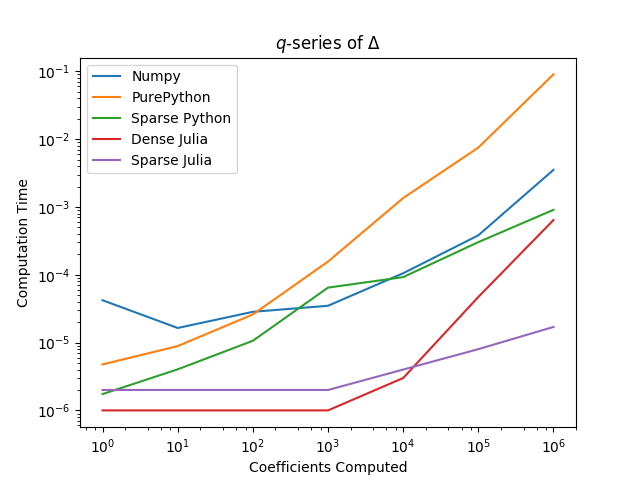
\includegraphics{speed_comparison_delta}

For small computations, the implementation doesn't make a big difference.
However, for large computations, it seems that the sparse methods do better.
It makes sense, since sparse representations are typically used for objects with more than 95\% of zeros, which is the case for modular forms modulo 2.

For a more precise analysis, we now compare the speed of each implementation to compute $q$-series of $\Delta$ and $\Delta^2$
\footnote{$\Delta^2$ itself isn't part of our space $\mathcal{F}$, but it will be useful as we will compute $\Delta^{2k+1} = \Delta^{2k-1}\cdot \Delta^2$. So it makes sense to be concerned about it.}.
The following table is obtained for $10^6$ coefficients computed (i.e. up to $q^{10^6}$).
Note that $\mathcal{O}(q^{10^6})$ will be standard for the rest of this paper.

\begin{center}
	\begin{tabular}{r||l|l}
		 & $\Delta$ & $\Delta^2$\\
		\hline\hline
		Pure Python   & 0.08263147 & 0.26249526 \\
		NumPy Python  & 0.00138761 & 0.16163688 \\
		Dense Julia   & 0.000648   & 0.001698   \\
		Sparse Python & 0.00095099 & 0.00134479 \\
		Sparse Julia  & 0.000021   & 0.000034   \\
	\end{tabular}
\end{center}

From this table, it is clear that the fastest implementation is the one using sparse lists (so called "sparse vectors") in Julia.
Therefore, we will use this technique.
It is nice to remark that the Pure Python implementation was 7720 times slower than the Sparse Julia one.
We see here the importance of choosing the right tool to implement an algorithm.

This ratio would even be greater considering the bad algorithm presented before \ref{algorithmOptimisation}.



\subsection{Creating the library}
It is clear now that the code should be done with Julia and it's Sparse objects.
Now, as all the library should be created from the beginning, it is a good idea to pack all of it in a Julia module.
Doing so, no code will be repeated for each small task.



\subsubsection[Main Module]{ModularFormsModuloTwo.jl}
The code will be divided in a many files, for convenience.

\paragraph{Code Architecture}
The main function are direct parts of the module, and the pre-calculated data part is written in a sub-folder, detailed next paragraph.
Here is a visualization of the organisation (the "architecture"):

% code architecture draw
\tikzset{
	file/.style={
		rectangle,
		rounded corners,
		draw=black, very thick,
		minimum height=4.2cm,
		minimum width=3.8cm,
		inner sep=2pt,
		text width=3.7cm,
	},
}
\tikzset{
	submodule/.style={
		rectangle,
		rounded corners,
		draw=black, thin,
		minimum height=1.5cm,
		minimum width=4.6cm,
		inner sep=2pt,
		text width=4.7cm,
	},
}
\begin{tikzpicture}
%% nodes
\coordinate(top) at (0,0);
\node[file, text width=6.25cm] (MFmod2) at (top){
	\begin{tabular}{l}
	\textbf{ModularFormsModuloTwo.jl}\\
	$\cdot$ ModularForm (\textit{type})\\
	$\cdot$ ModularFormList (\textit{type})\\
	$\cdot$ \textit{Printing functions}\\
	\\
	\\
	\\
	\end{tabular}
};
\node[file, below of = top, node distance=5cm] (gene){
	\begin{tabular}{l}
	\textbf{generator.jl}\\
	$\cdot$ zero ($0$)\\
	$\cdot$ one ($1$)\\
	$\cdot$ delta ($\Delta$)\\
	$\cdot$ delta\_k ($\Delta^k$)\\
	\\
	\\
	\end{tabular}
};
\node[file, left of = gene, node distance=4cm] (arithm){
	\begin{tabular}{l}
	\textbf{arithmetic.jl}\\
	$\cdot$ addition ($+$)\\
	$\cdot$ multiplication ($*$)\\
	$\cdot$ square (²)\\
	$\cdot$ power (${}^{\boxed{}}$)\\
	\textbf{equality.jl}\\
	$\cdot$ eq ($\overset{?}{=}$)\\
	\end{tabular}
};
\node[file, right of = gene ,node distance=4cm] (reco){
	\begin{tabular}{l}
	\textbf{recognizer.jl}\\
	$\cdot$ to\_q ($\Delta \to q$)\\
	$\cdot$ to\_$\Delta$ ($q \to \Delta$)\\
	$\cdot$ drop\_error ($q \circlearrowleft$)\\
	\\
	\\
	\\
	\end{tabular}
};
\node[file, right of = reco, node distance=4.5cm] (Hecke){
	\begin{tabular}{l}
	\textbf{HeckeOperator.jl}\\
	$\cdot$ Hecke ($T_p$)\\
	\\
	\\
	\\
	\\
	\end{tabular}
};
\node[submodule, right of = MFmod2, node distance=7cm, thin] (Data){
	\begin{tabular}{l}
	\textbf{Data (submodule)}\\
	\textit{(load precalculated data)}\\
	\end{tabular}
};
%% links
\path (MFmod2) edge (arithm);
\path (MFmod2) edge (gene);
\path (MFmod2) edge (reco);
%\path (MFmod2) edge (Hecke);
\path (MFmod2) edge (+6,-2);
\path (+6,-2) edge (Hecke);
\path (MFmod2) edge (Data);
\end{tikzpicture}
\begin{center}
	Major functions of the module and their repartitions into file (represented by boxes).
\end{center}



\paragraph{Files Details}
We will detail here the important and interesting parts of the code.
For more details, the reader may refer to the source code, witch is commented and documented.
\subparagraph{Basics Operations}
Basic operations on modular forms modulo 2 are defined in \texttt{arithmetic.jl} (see \ref{code:arithmetic} or \url{https://github.com/pauldubois98/ModularFormsModuloTwo.jl/blob/master/src/arithmetic.jl}).
All of these algorithms have been optimised as much as possible (i.e. cutting loops as soon as possible, and iterate through "ones" only, as most coefficients are zero).
\subparagraph{Equality up to known}
It might be useful to compare two modular form up to some coefficients (perhaps if $f_1$ is known up to $q^n$ and $f_2$ up to $q^m$, we can compare them up to $q^{\min{n,m}}$).
This equality test is defined in \texttt{equality.jl} (see \ref{code:equality} or \url{https://github.com/pauldubois98/ModularFormsModuloTwo.jl/blob/master/src/equality.jl}).
\subparagraph{Generators of $\mathcal{F}$}
As modular forms modulo 2 are polynomials of $\Delta$, we need to ba able to generate the $q$-series of powers of $\Delta$.
Such functions are defined in \texttt{generator.jl} \footnote{\texttt{generators.jl} generates $\Delta$ and then uses the power function from \texttt{arithmetic.jl}.} (see \ref{code:generators} or \url{https://github.com/pauldubois98/ModularFormsModuloTwo.jl/blob/master/src/generators.jl}).
Here, the optimization is not trivial:
To calculate $\Delta^{31}$ (say), the most trivial way is to do $\Delta \cdot \Delta \cdots \Delta$ with 30 multiplications.
But what is done in fact inside the library is much faster: we calculate $\Delta$, $\Delta^2 = \Delta \cdot \Delta$, $\Delta^4 = \Delta^2 \cdot \Delta^2$, ... until $\Delta^{16}$, and then $\Delta^{31} = \Delta^{16} \cdot \Delta^8 \cdot \Delta^4 \cdot \Delta^2 \cdot \Delta$.
Doing like this, only 8 multiplications were needed (against 30 with the naïve method).
On may think that 3 was an example particularly good for this technique, but if we take another example, say 32, we would turn 31 multiplication to 5.
In fact, in general, to calculate $\Delta^n$ this second method need a maximum of $\log_2(n)^2$ multiplications against $n-1$ for the first one.
So it really is a much faster algorithm.\footnote{In fact, half of the operations are squaring modular forms, which is much faster than a usual multiplication. This this algorithm is even better than stated.}
\subparagraph{Hecke Operators}
The only formula we have to calculate Hecke operators, is using the $q$-representation of modular forms.
Therefore, the Hecke operators are taking a modular forms under $q$-representation as input (together with a prime $p$).
Note that when applying a Hecke operator, we loose a lot of informations on it's expansion:
If $f$ is known up to $q^n$, then $T_p|f$ will only be known up to $q^{n/p}$.
This means that we should be careful when applying Hecke operator.

Hecke operators are implemented in the file \texttt{HeckeOperator.jl} (see \ref{code:HeckeOperator} or \url{https://github.com/pauldubois98/ModularFormsModuloTwo.jl/blob/master/src/HeckeOperator.jl})
\subparagraph{Recognise the trick?}
\label{recogniseTrick}
This part of the module us probably the most important, and it is the one that differ the most form any other computing technique.

We start by noting that it is easy to go from the $\Delta$ representation of a modular form to the $q$ representation: it suffices to choose an arbitrary $n$, and calculate all coefficients up to $q^n$, using the series expansion of $\Delta$.
This step is necessary to calculate Hecke operators.

Now, one may ask if it is possible to go back from the $q$-representation to the $\Delta$-representation of a modular form.
In general, this is not possible.
\textbf{But}
If we have some assumptions on the modular form, then it may become possible.
For example, if we know that the maximum degree (in terms of $\Delta$) of $f$ is n, and that we know it's $q$-coefficients up to n:
then $f$ may be written as $f = \sum_{k \leq n} \mu_k \Delta^k$, so the set $\{ \Delta^k | k \leq n \}$ acts as a basis, and it is just a matter of finding the matching coefficients $\mu_k$.
This is in fact possible, and that is how the function \texttt{to\_delta()} is made possible.

Now, once we have the $\Delta$ representation of a modular form, we potentially have as many $q$-coefficients as we want.
This may seem weird or even magical, since we assumed only finitely many $q$-coefficients were known.
In fact, we can use this fact to drop the numerical error that calculating a Hecke operator may have produced.

Such kind of calculations are rather unusual in computer science: usually computers approximates objects, and this approximation error is never given back.
But with modular forms modulo two, we can take back the approximation error.

This method will now be referred as exact computations. [may I create this name?]

It is implemented in the file \texttt{recognizer.jl} (see \ref{code:recognizer} or \url{https://github.com/pauldubois98/ModularFormsModuloTwo.jl/blob/master/src/recognizer.jl}).
\subparagraph{Global}
The last file, \texttt{ModularFormsModuloTwo.jl} is the one that creates the link between all the small part of programs written in other files.
It also defines a few general objects, such as types and printing functions.
For more details, see (\ref{code:ModularFormsModuloTwo} or \url{https://github.com/pauldubois98/ModularFormsModuloTwo.jl/blob/master/src/ModularFormsModuloTwo.jl})
\subsubsection[Sub Module]{(Pre-calculated) Data}
Data is natively part of the ModularFormModuloTwo.jl module, but it is treated internally as a sub-component, for better organisation.



\paragraph{Code Architecture}
This time, the architecture is much easier:

\tikzset{
	subfile/.style={
		rectangle,
		rounded corners,
		draw=black, very thick,
		minimum height=1.2cm,
		minimum width=5.2cm,
		inner sep=2pt,
		text width=5.5cm,
		align=center,
	},
}
\begin{tikzpicture}
%% nodes
\coordinate(top) at (0,0);
\node[submodule, align=center] (data) at (top){
	\textbf{\LARGE Data}
};
\node[subfile, below of = top, node distance=3cm] (storage){
	storage.jl
};
\node[subfile, right of = storage, node distance=6cm] (delta){
	delta\_file\_maker.jl
};
\node[subfile, right of = delta ,node distance=6cm] (primes){
	Hecke\_primes\_file\_maker.jl
};
\node[subfile, above of = primes, node distance=3cm] (powers){
	Hecke\_powers\_file\_maker.jl
};
%% links
\path (data) edge (storage);
\path (data) edge (delta);
\path (data) edge (primes);
\path (data) edge (powers);
\end{tikzpicture}

\paragraph{Files Details}
We will detail here an overview of what each file achieve.
For more details, the reader may look at the source code, which is highly commented, and quite explicit in general.
\begin{itemize}
	\item \texttt{storage.jl} (see \ref{code:storage} or \url{https://github.com/pauldubois98/ModularFormsModuloTwo.jl/blob/master/src/data/storage.jl}): This is the only file to be called outside of the Data sub-module.
	\item \texttt{delta\_file\_maker.jl} (see \ref{code:deltaFileMaker} or \url{https://github.com/pauldubois98/ModularFormsModuloTwo.jl/blob/master/src/data/delta_file_maker.jl}): The program in this file generates the $q$-coefficients lists for a range of powers of $\Delta$.
	\item \texttt{Hecke\_primes\_file\_maker.jl} (see \ref{code:HeckePrimesFileMaker} or \url{https://github.com/pauldubois98/ModularFormsModuloTwo.jl/blob/master/src/data/Hecke_primes_file_maker.jl}): The program in this file calculates the $\Delta$-representation lists for a range of Hecke operators $T_p$ and range of powers of $\Delta$.
	\item \texttt{Hecke\_powers\_file\_maker.jl} (see \ref{code:HeckePowersFileMaker} or \url{https://github.com/pauldubois98/ModularFormsModuloTwo.jl/blob/master/src/data/Hecke_powers_file_maker.jl}): The program in this file calculates the $\Delta$-representation lists for a range of powers of Hecke operators $T_3$ and $T_5$ and range of powers of $\Delta$.
\end{itemize}



\subsubsection{Open-Source}
This library is completely open-source.
Anyone is welcome to contribute.
Anyone can use it (for free).

\subsubsection{Official}
This module is now registered as an official Julia package.
To use all the code form this library, a new user will just need to type:
\begin{minted}{julia}
julia> using Pkg
julia> Pkg.add(PackageSpec(url="https://github.com/pauldubois98/ModularFormsModuloTwo.jl"))
\end{minted}
It is convenient that all the algorithms developed in this module can be used just by importing the package, which can be done in a minute.

\subsubsection{Online Documentation}
As it usually comes wit open-sources packages, ModularFormsModuloTwo.jl has an \href{https://pauldubois98.github.io/ModularFormsModuloTwo.jl/}{online documentation} (see \url{https://pauldubois98.github.io/ModularFormsModuloTwo.jl/}).




\subsection{Finding Coefficients $a_{ij}(p)$}
\label{finding_a_ij(p)}
\subsubsection{Strategy}
We want to find the coefficients $a_{ij}$ such that 
\begin{equation}
\label{eq:coefficientsEquate}
	T_p = \sum_{i+j \geq 1} a_{ij}(p)T_3^iT_5^j \tag{$*$}
\end{equation}
(with $a_{ij}(p) \in \mathbb{F}_2$).
Note that this is a finite sum, since Hecke operators are nilpotent.

The strategy is as follows: we use the module we developed.
It allows us to compute the (exact) $\Delta$-representation of $T_p|\Delta^k$ and $\sum_{i+j \geq 1} a_{ij}(p) T_3^iT_5^j|\Delta^k$ for many $k$, $p$, $i$ and $j$.
Now, since \eqref{eq:coefficientsEquate} should hold for all modular forms $f \in \mathcal{F}$, it has to holds, in particular, for all $\Delta^k$ (with $k$ and odd integer).
Thus, we will plug successive $\Delta^k$ and equate coefficients.
This will eventually give all $a_ij(p)$.

\subsubsection{Algorithm}
As explained before, we plot $\Delta^k$ successively for a range of $k$.
In reality, most of the terms of the sum in \ref{eq:coefficientsEquate} are zeros.
This is both nice and not good:
It is nice because it makes the system is easy to solve.
But it also makes all coefficients in front of zeros terms being undetermined.
This implies that we need to plug larger powers of $\Delta$ to fix coefficients.
And bigger powers of $\Delta$ ask for heavier computations (and now we see how important it was to optimize the modular forms modulo 2 module).

As this algorithm is the heart of all computations, we give a pseudo-code simplified version:
\begin{algorithmic}
	\color{CodeColor}
	\Require $MAX_K$ \Comment{Maximum power $\Delta^k$ for which $T_p|\Delta^k$ and $T_3^iT_5^j|\Delta^k$ are known (computed)}
	\Require $MAX_I$ \Comment{Minimum $i \in \N$ such that $T_3^i|\Delta^{MAX_K} \neq 0$}
	\Require $MAX_J$ \Comment{Minimum $j \in \N$ such that $T_5^j|\Delta^{MAX_K} \neq 0$}
	\ForAll{$p \in \primes$, $p>2$}
		\Comment{We compute the map $a_{ij}(p)$ for each specific odd $p$ prime}
		\State{$a_p$ is a $MAX_I \times MAX_J$ 2-dimensional matrix} \Comment{$a_p[i,j]$ will correspond to $a_{ij}(p)$}
		\State{Fill $a_p$ for known values (i.e. for $i+j \leq 2$}
		\For{$k < MAX_K$}
			\State{$f = T_p|\Delta^k$}
			\State{$LIST_a$} \Comment{The list of $a_p[i,j]$ to fix using $\Delta^k$ iteration}
			\State{$LIST_f$} \Comment{The corresponding list of modular forms $T_3^iT_5^j|\Delta^k$}
			\For{$0 \leq i \leq MAX_I$}
				\For{$0 \leq j \leq MAX_J$}
					\If{$a_p[i,j]=1$}
						\State{$f += T_3^iT_5^j|\Delta^k$} \Comment{Add $1 * T_3^iT_5^j|\Delta^k$ to $f$}
					\ElsIf{$a_p[i,j]=0$}
						\State{Pass} \Comment{Add $0 * T_3^iT_5^j|\Delta^k$ to $f$}
					\Else \Comment{$a_p[i,j]$ is unset in this case.}
						\State{Append $a_p[i,j]$ to $LIST_a$} \Comment{We add $a_p[i,j]$ to the list}
						\State{Append $T_3^iT_5^j|\Delta^k$ to $LIST_f$} \Comment{We add $T_3^iT_5^j|\Delta^k$ to the list}
					\EndIf
				\EndFor
			\EndFor
			\State{Find $a_p[i,j]$ in $LIST_a$ that solve that system $f = \sum a_p[i,j] T_3^iT_5^j|\Delta^k$} \Comment{using built-in linear solver, for efficiency}
		\EndFor
		\State{Output $a_p$}
	\EndFor
\end{algorithmic}
The implementation of this algorithm (in Julia) is in \ref{code:a_ij(p)calculation}.



\subsubsection{Computations Limitations}
Here, we discuss the bounds to put in the algorithm, for a decent amount of data, and a descent amount of computation time.

\paragraph{Computing Hecke of Large Primes Versus Large Powers}
Here, we compare the difficulty to compute Hecke operators for large primes ($T_p$ for $p >> 2$), against the difficulty to compute Hecke operators for large powers of Hecke operators ($T_3^iT_5^j$ for $i,j >> 1$).

\subparagraph{Computing Hecke Operators for Large Primes}
When calculating a Hecke operator $T_p$ for a modular form $f$, the maximum known coefficient is $q^{\frac{N}{p}}$ if $f$ is known for coefficients up to $q^{N}$.
This means that we can compute the $\Delta$ representation for $T_p|f$ only if we know it will have a degree (in terms of $\Delta$) of maximum $\frac{N}{p}$.
Thus, if we choose to compute $a_{ij}(p)$ for $p \leq P$, it means that $\degree{T_p|f} \leq \frac{N}{P} = K$.

\subparagraph{Computing Hecke Operators for Large Powers}
Now, at a first thought, $T_p$ isn't too pathological compared to $T_3^iT_5^j$ for large $i$ and $j$, since the maximum known coefficient would be $q^{\frac{N}{3^i5^j}}$ if $f$ is known for coefficients up to $q^{N}$.

But in fact, we can apply a trick here:
Once we know $T_3|f$ (once we computed it's $q$-representation), we straight calculate the $\Delta$-representation, and then get back to the $q$-representation with no "lose of coefficients".
This may look weird at first, since we have the $q$-representation of $T_3|f$, and we need it to calculate $T_3^2|f$.
However, we known the $q$-representation of $T_3|f$ with some coefficients lost.
And the fact that we go back to the $\Delta$-representation allows us to drop the numerical error.
Doing this again and again, there is no lose at all in the coefficients calculated.

This is why exact computations (this is the name we gave to this trick) is crucial for this algorithm.
In fact, for powers of Hecke operators, we only need to compute the $q$-representations of modular forms up to $5 \ \degree{f}$, since each $T_3$ or $T_5$ will lose at most $\nicefrac{4}{5}$ of the $q$-coefficients.

\subparagraph{Conclusion}
Thus, the part which use to be the most pathological in fact becomes much nicer than the other: calculating Hecke operators for large powers is easier than for large primes.

\paragraph{Reasonable Bounds}
Here, we give limits used in the actual computations.

It seems that using $q$ series capped at $q^{10^6}$ is reasonable (i.e. computations will be a few days long).
We would like to compute $a_ij(p)$ for small $i,j$ and $p \leq 10^4$.

So the setup (in the same notation as above) is $N=10^6$, $P=10^4$, so $K=10^2$.
Then the algorithm will compute as much $a_{ij}(p)$ as possible, for each $p \leq P$.
This maximum can in fact be calculated implicitly:
$a_{ij}(p)$ will be computed if and only if $T_3^iT_5^j|f$ is non-zero for one of the forms $f$ plugged.
As we plug powers of $\Delta$ up to $K$, this means $a_{ij}(p)$ will be computed for all $p \leq P$ if and only if $k \leq K$, where $k$ is the odd integer with code $[i,j]$.

\subsubsection{Results}
Here, we will give results for the prime $p=19$.
There are many links in this section, if the reader in interested in all the data calculated (it won't fit in this paper).

\paragraph{Expansions of $T_p$}
We have the following extension:
$$
T_{19} = T_3^1T_5^0 + T_3^3T_5^0 + T_3^1T_5^4 + T_3^3T_5^2 + T_3^1T_5^6 + T_3^5T_5^2 + T_3^3T_5^6 + T_3^7T_5^2 + T_3^9T_5^0 + \dots
% + T_3^1T_5^{10} + T_3^7T_5^4 + T_3^9T_5^2 + T_3^{11}T_5^0
% + T_3^1T_5^{12} + T_3^5T_5^8 + T_3^{11}T_5^2 + T_3^{13}T_5^0 + T_3^3T_5^{12} + T_3^7T_5^8 + T_3^9T_5^6 + T_3^{11}T_5^4 + T_3^{13}T_5^2 + T_3^3T_5^{14} + T_3^7T_5^{10} + T_3^{11}T_5^6 + T_3^{15}T_5^2 + T_3^{17}T_5^0
$$
Writing $x = T_3$ and $y = T_5$, this is:
$$
T_{19} = x^1y^0 + x^3y^0 + x^1y^4 + x^3y^2 + x^1y^6 + x^5y^2 + x^3y^6 + x^7y^2 + x^9y^0 + x^1y^{10} + x^7y^4 + x^9y^2 + x^{11}y^0 + \dots
% + x^1y^{12} + x^5y^8 + x^{11}y^2 + x^{13}y^0 + x^3y^{12} + x^7y^8 + x^9y^6 + x^{11}y^4 + x^{13}y^2 + x^3y^{14} + x^7y^{10} + x^{11}y^6 + x^{15}y^2 + x^{17}y^0
$$
For expansions of other primes, please visit \href{https://pauldubois98.github.io/HeckeOperatorsModuloTwo/T_p_extensions/}{this web site}:\\ \url{https://pauldubois98.github.io/HeckeOperatorsModuloTwo/T_p_extensions/}.

For $p=19$, we can also look at $a_{ij}(p)$ as an infinite 2-dimensional table:
\begin{center}
	\begin{tabular}{|c||c|c|c|c|c|c|c|c|c|c|c|c|c|c|c|c|}
		\hline
		\textbf{$ T_19$} & \textbf{$ T_5^{0} $} & \textbf{$ T_5^{1} $} & \textbf{$ T_5^{2} $} & \textbf{$ T_5^{3} $} & \textbf{$ T_5^{4} $} & \textbf{$ T_5^{5} $} & \textbf{$ T_5^{6} $} & \textbf{$ T_5^{7} $} & \textbf{$ T_5^{8} $} & \textbf{$ T_5^{9} $} & \textbf{$ T_5^{10} $} & \textbf{$ T_5^{11} $} & \textbf{$ T_5^{12} $} & \textbf{$ T_5^{13} $} & \textbf{$ T_5^{14} $} & \textbf{$ T_5^{15} $} \\
		\hline
		$ T_3^{0} $ & 0 & 0 & 0 & 0 & 0 & 0 & 0 & 0 & 0 & 0 & 0 & 0 & 0 & 0 & 0 & 0 \\
		$ T_3^{1} $ & 1 & 0 & 0 & 0 & 1 & 0 & 1 & 0 & 0 & 0 & 1 & 0 & 1 & 0 & 0 & 0 \\
		$ T_3^{2} $ & 0 & 0 & 0 & 0 & 0 & 0 & 0 & 0 & 0 & 0 & 0 & 0 & 0 & 0 & 0 & 0 \\
		$ T_3^{3} $ & 1 & 0 & 1 & 0 & 0 & 0 & 1 & 0 & 0 & 0 & 0 & 0 & 1 & 0 & 1 & 0 \\
		$ T_3^{4} $ & 0 & 0 & 0 & 0 & 0 & 0 & 0 & 0 & 0 & 0 & 0 & 0 & 0 & 0 & 0 &  \\
		$ T_3^{5} $ & 0 & 0 & 1 & 0 & 0 & 0 & 0 & 0 & 1 & 0 & 0 & 0 & 0 & 0 &  &  \\
		$ T_3^{6} $ & 0 & 0 & 0 & 0 & 0 & 0 & 0 & 0 & 0 & 0 & 0 & 0 & 0 &  &  &  \\
		$ T_3^{7} $ & 0 & 0 & 1 & 0 & 1 & 0 & 0 & 0 & 1 & 0 & 1 & 0 &  &  &  &  \\
		$ T_3^{8} $ & 0 & 0 & 0 & 0 & 0 & 0 & 0 & 0 & 0 & 0 & 0 &  &  &  &  &  \\
		$ T_3^{9} $ & 1 & 0 & 1 & 0 & 0 & 0 & 1 & 0 & 0 & 0 &  &  &  &  &  &  \\
		$ T_3^{10} $ & 0 & 0 & 0 & 0 & 0 & 0 & 0 & 0 & 0 &  &  &  &  &  &  &  \\
		$ T_3^{11} $ & 1 & 0 & 1 & 0 & 1 & 0 & 1 & 0 &  &  &  &  &  &  &  &  \\
		$ T_3^{12} $ & 0 & 0 & 0 & 0 & 0 & 0 & 0 &  &  &  &  &  &  &  &  &  \\
		$ T_3^{13} $ & 1 & 0 & 1 & 0 & 0 & 0 &  &  &  &  &  &  &  &  &  &  \\
		$ T_3^{14} $ & 0 & 0 & 0 & 0 & 0 &  &  &  &  &  &  &  &  &  &  &  \\
		$ T_3^{15} $ & 0 & 0 & 1 & 0 &  &  &  &  &  &  &  &  &  &  &  &  \\
		$ T_3^{16} $ & 0 & 0 & 0 &  &  &  &  &  &  &  &  &  &  &  &  &  \\
		$ T_3^{17} $ & 1 & 0 &  &  &  &  &  &  &  &  &  &  &  &  &  &  \\
		$ T_3^{18} $ & 0 &  &  &  &  &  &  &  &  &  &  &  &  &  &  &  \\
		\hline
	\end{tabular}

	Here, blanks are coefficients not computed.
\end{center}
For tables of other primes, please visit \href{https://pauldubois98.github.io/HeckeOperatorsModuloTwo/a_ij_p/}{this web site}:\\ \url{https://pauldubois98.github.io/HeckeOperatorsModuloTwo/a_ij_p/}.

Now, we will later be interested in the map $p \mapsto a_{ij}(p)$, so it makes sense for each pair $(i,j)$, to list the \textit{1-primes} (i.e. the set $\{ p \in \primes \mid a_{ij}(p) = 1 \}$) or the 0-primes 
This is what we do in the following table:
\begin{center}
	\begin{tabular}{|r|l|}
		\hline
		\textbf{$a_{ij}$} & \textbf{$ \lbrace p \in \primes \mid a_{ij}(p) = 1 \rbrace $} \\
		\hline
		$ a_{0 1} $ & 5, 13, 29, 37, 53, 61, 101, 109, 149, 157, 173, 181, 197, 229, 269, 277, 293, 317, 349, ...\\
		$ a_{1 0} $ & 3, 11, 19, 43, 59, 67, 83, 107, 131, 139, 163, 179, 211, 227, 251, 283, 307, 331, 347, ...\\    
		$ a_{0 2} $ & 17, 41, 97, 137, 193, 241, 313, 401, 409, 433, 449, 457, 521, 569, 641, 673, 761, 769, ...\\
		$ a_{1 1} $ & 7, 23, 31, 47, 71, 79, 103, 127, 151, 167, 191, 199, 223, 239, 263, 271, 311, 359, 367, ...\\
		$ a_{2 0} $ & 17, 73, 89, 97, 193, 233, 241, 281, 401, 433, 449, 601, 617, 641, 673, 769, 929, 937, ...\\
		$ a_{0 3} $ & 13, 29, 37, 101, 149, 173, 181, 317, 349, 389, 557, 661, 677, 709, 733, 757, 773, 997, ...\\
		$ a_{1 2} $ & 11, 59, 67, 83, 107, 131, 179, 211, 251, 331, 347, 379, 419, 499, 523, 547, 587, 619, ...\\
		$ a_{2 1} $ & 13, 37, 53, 61, 101, 157, 173, 277, 373, 389, 509, 541, 557, 677, 701, 709, 773, 797, ...\\
		$ a_{3 0} $ & 11, 19, 67, 107, 131, 283, 307, 331, 419, 443, 467, 523, 547, 563, 571, 587, 619, 643, ...\\
		$ a_{0 4} $ & 73, 89, 113, 233, 353, 577, 593, 601, 937, 1153, 1201, 1289, 1433, 1601, 1609, 1721, ...\\
		$ a_{1 3} $ & 23, 31, 71, 79, 103, 127, 151, 191, 223, 239, 263, 359, 431, 463, 479, 503, 631, 647, ...\\
		$ a_{2 2} $ & 17, 41, 73, 89, 113, 233, 241, 257, 313, 353, 401, 409, 433, 457, 601, 761, 809, 937, ...\\
		$ a_{3 1} $ & 7, 79, 167, 199, 239, 311, 383, 431, 439, 463, 487, 599, 607, 719, 727, 743, 751, 823, ...\\
		$ a_{4 0} $ & 41, 113, 257, 313, 337, 409, 457, 577, 761, 809, 881, 1129, 1249, 1553, 1657, 1889, ...\\
		$ a_{0 5} $ & 13, 53, 61, 101, 109, 157, 173, 197, 269, 317, 349, 389, 421, 461, 613, 653, 661, 701, ...\\
		$ a_{1 4} $ & 11, 19, 67, 107, 131, 163, 179, 211, 227, 251, 283, 307, 331, 347, 419, 491, 643, 811, ...\\
		$ a_{2 3} $ & 29, 37, 53, 61, 101, 149, 157, 173, 197, 269, 293, 389, 397, 421, 541, 557, 613, 653, ...\\       
		$ a_{3 2} $ & 11, 19, 43, 83, 107, 131, 163, 211, 251, 347, 379, 419, 443, 467, 491, 523, 563, 571, ...\\
		$ a_{4 1} $ & 13, 53, 101, 149, 157, 173, 181, 229, 317, 373, 397, 421, 461, 613, 661, 701, 709, ...\\
		$ a_{5 0} $ & 11, 43, 59, 67, 83, 139, 163, 251, 283, 419, 467, 499, 547, 587, 619, 643, 659, 811, ...\\
		$ \dots $ & \\
		\hline
	\end{tabular}

	Table of 1-primes
\end{center}
Again, for complete tables, please visit \href{https://pauldubois98.github.io/HeckeOperatorsModuloTwo/a_ij_p/a_ij_p-1.html}{this web site}:\\ \url{https://pauldubois98.github.io/HeckeOperatorsModuloTwo/a_ij_p/a_ij_p-1.html}.

Note that tables for \textit{0-primes} (i.e. the set $\{ p \in \primes \mid a_{ij}(p) = 0 \}$) may be found \href{https://pauldubois98.github.io/HeckeOperatorsModuloTwo/a_ij_p/a_ij_p-0.html}{here}:\\
\url{https://pauldubois98.github.io/HeckeOperatorsModuloTwo/a_ij_p/a_ij_p-0.html}.




\subsection{Finding Governing Fields}
\label{numerics:GoverningFields}
\subsubsection{Computations Strategy}
As it is usually the case with computations, this algorithm will not give a proof that the considered field is a governing field.
What we will do, is to check that for sufficiently many primes, the field we consider is a governing field.

\paragraph{Algorithm}
\subparagraph{Outline}
Consider the field $L$ extending $\Q$, suppose we suspect it to be a governing field for $a_{ij}$.
We want to check that there exists a subset $S \subseteq G = \Gal{L/\Q}$ that is stable under conjugacy, such that $\Frob{L/\Q}{p} \in S$ if and only if $a_{ij}(p)=1$.
That is $\Frob{L/\Q}{p} \in S$ if $a_{ij}(p)=1$ and $\Frob{L/\Q}{p} \not \in S$ if $a_{ij}(p)=0$.

\subparagraph{Pseudo-code}
\label{algo:governingFieldsChecks}
Here is a pseudo-code version of the algorithm used:
\begin{algorithmic}
	\color{CodeColor}
	\State{$MAX_P \in \N$}
	\State{$i,j \in \N$ given}
	\State{$L$ a given  number field, suspected to be a governing field for $a_{ij}$.}
	\State{$G = \Gal{L/\Q}$}
	\State{$Primes-1$ an empty set.}
	\For{$p \in \primes, p<MAX_P, a_{ij}(p)=1$}
		\If{$\Frob{L/\Q}{p} \in Primes-0$}
			\State{Add $\Frob{L/\Q}{p}$ to the set $Primes-1$}
		\EndIf
	\EndFor
	\For{$p \in \primes, p<MAX_P, a_{ij}(p)=0$}
		\If{$\exists F_q \in Primes-0 \text{ s.t. } \Frob{L/\Q}{p} \sim F_q$}
			\State{REJECT!}
		\EndIf
	\EndFor
	\Comment{Accept as not rejected yet.}
	\State{$L$ is a Governing field for $a_{ij}$.}
\end{algorithmic}
The implementation of this algorithm (in Python) is in \ref{code:governingFieldsChecks}.
Note that the hardest part to program is in fact the transition between computer's representation of mathematical objects, and the human readable versions. This part isn't mathematically interesting, so has been hidden in this paper. The interested reader may find complete programs on GitHub (see \url{https://github.com/pauldubois98/HeckeOperatorsModuloTwo/tree/master/GoverningFields}).

\paragraph{Implementation Strategy}
For algebraic computations (such as computing Frobenius elements), many libraries already exist.
However, many (such as SageMath) are limited in terms of degree of field extensions.
This is why we will use a very powerful and respected library: PARI GP.
PARI GP may be used through C, but for simplicity, we will use the the GP language that PARI GP developers suggest.

It isn't easy to connect the Julia computations for the maps $a_{ij}$ and the PARI GP language.
So we will export results from both sides in text files, and analyse it with Python.
Note here that the analysis is just checking if whether or not, the field is a governing field.
All the "difficult" computations are made in very efficient languages (Julia and the highly optimized PARI GP library).
So it is fine, for convenience, to use a slower language as Python for the last step, which isn't computationally fast.

\subsubsection{Reliability}
We want the program elaborated to be reliable.
Since we are mixing 3 different languages (PARI GP, Python, and Julia), it isn't easy to check that no error was made when coding.

\paragraph{Checking on Known Governing Fields}
This is the reason why we first check that the fields $\Q(\zeta_8, \sqrt[4]{2})$, $\Q(\zeta_8, \sqrt{1+i})$, and $\Q(\zeta_{16})$ are validated by the program as governing fields for $a_{02}$, $a_{20}$, and $a_{11}$.
Even if maths is an exact science (so we don't need to check again some result found before), it is still nice to see that the theory is consistent.

Unsurprisingly, we in fact find results expected form \cite[§7]{StructureAlgebreHecke}.

\paragraph{New Governing Fields}
We apply the exact same method as before, and find very good candidates governing fields for: $a_{03}$, $a_{04}$, $a_{05}$, $a_{06}$, $a_{07}$, $a_{30}$, $a_{40}$, $a_{50}$, $a_{60}$, and $a_{70}$.
We also have some less reliable results for $a_{08}$ and $a_{80}$.
All the details can be found in \ref{governingFieldsResults}.



\subsection{Probabilistic graphs}
ASSUMING [BLA]
... we can produce plots of $a_ij(p)$ to check it has th right distribution....
Here, we look for the probability that the results found appeared randomly.
We assume that the Frobenius element of a prime is random for each prime.
then the proba [bla].
[this part is written, but only in my head, at the moment.]







\bibliography{references}
\bibliographystyle{alpha}

\end{document}
